\documentclass[11pt]{article}

% --- Geometry: ~6.5 inch text width matches matplotlib defaults in cf.viz ---
\usepackage[a4paper, margin=1in]{geometry}

% --- Math, graphics, tables ---
\usepackage{amsmath}
\usepackage{amssymb}
\usepackage{graphicx}
\usepackage{booktabs}
\usepackage{array}
\usepackage{tabularx}
\usepackage{float}
\usepackage{caption}
\usepackage{subcaption}
\usepackage{microtype}

% --- Cross references ---
\usepackage[hidelinks]{hyperref}
\usepackage[noabbrev,capitalise]{cleveref}

% --- Figures live in report/figures/ ---
\graphicspath{{figures/}}

% --- Section formatting: prefix top-level headings with "Section",
%     keep subsection numbering as 1.1 / 1.2 / etc., start every
%     top-level section on a fresh page. ---
\usepackage{titlesec}
\titleformat{\section}[hang]
  {\normalfont\Large\bfseries}{Section \thesection.}{0.6em}{}
\titlespacing*{\section}{0pt}{0pt}{12pt}
\titlespacing*{\subsection}{0pt}{12pt}{6pt}

% Force every \section to start on a new page
\let\oldsection\section
\renewcommand{\section}{\clearpage\oldsection}

\begin{document}

\begin{titlepage}
    \centering
    \vspace*{2cm}

    {\Huge \textbf{Hedge Fund\\
    Panel Time Series Forecasting}}\\[1cm]

    {\Large \textbf{Course Name:} Applied Forecasting Methods}\\[2cm]

    {\Large \textbf{Group-8 Members:}}\\[0.5cm]
    Kaushal Nandaniya (202303036)\\[0.2cm]
    Jeetrajsinh Gohil (202303017)\\[0.2cm]
    Dhyey Patel (202301415)\\[0.2cm]
    Manthan Gajera (202301488)\\[2cm]

    {\Large \textbf{Instructor Name:} Prof. Pritam Anand}\\[2cm]

    {\Large \textbf{Institution Name:} Dhirubhai Ambani Institute of Information and Communication Technology}\\[2cm]

    {\Large \textbf{Github Repo:} \href{https://github.com/kaushalnandaniya/HedgeFund_TimeSeriesForcasting}{GitHub}}\\[2cm]

    \vfill
\end{titlepage}

\begin{abstract}
This project addresses a large-scale panel time-series forecasting problem derived from anonymised hedge-fund data, where the objective is to predict future values of a target variable across multiple heterogeneous series under a weighted evaluation metric. The problem is challenging due to heavy-tailed distributions, extreme weight concentration, non-stationarity, and varying lengths of historical data across series.
\\
\\
The study adopts a diagnostic-driven approach, beginning with extensive exploratory data analysis to understand missingness patterns, distributional properties, and weight imbalance. Stationarity is assessed using ADF and KPSS tests, followed by first differencing to stabilise the series. Classical forecasting models , smoothing, AR, MA, ARMA, and ARIMA , are applied to four representative series selected to span the panel's stress dimensions of length, volatility, and weight. In parallel, deep recurrent models (RNN, GRU, LSTM) are fit on the same series under adaptive chronological splits, and a global LightGBM model is fit under quantile loss with calibrated $80\%$ prediction intervals selected on a per-series basis through a rolling 70/20/20 chronological backtest.
\\
\\
The results demonstrate that no single model universally outperforms others across all series. Simple smoothing methods dominate on stable low-variance series; differenced ARIMA and short-lag AR dominate on the volatile and high-weight series under classical fitting; recurrent models add a further lift on those same informative series; and the LightGBM quantile method produces the strongest single point forecast on the highest-weight series ($\text{skill} = 0.865$) while delivering empirically calibrated intervals between $0.762$ and $0.862$ wPICP across all four representative series. The findings highlight the importance of aligning model choice with data characteristics and evaluation metrics.
\\
\\
Overall, this work emphasises that effective hedge-fund forecasting requires a combination of statistical diagnostics, model adaptability, and careful consideration of panel heterogeneity, and that the deployable artefact is a calibrated interval rather than a single point estimate.
\end{abstract}

\clearpage
\tableofcontents

\section{Introduction}
\label{sec:problem}

\subsection{Background and Motivation}
\label{sec:intro:background}

Hedge funds rely heavily on quantitative forecasting models to anticipate the behaviour of large numbers of financial instruments simultaneously. These predictions directly influence portfolio allocation, risk management, and trading strategies, making forecasting accuracy not merely a statistical objective but a driver of real financial outcomes. In modern quantitative finance, even marginal improvements in predictive performance can translate into substantial economic gains due to leverage, compounding, and high-frequency decision-making.

The forecasting problem at this scale has three properties that make it a useful subject for an applied forecasting study: panels of thousands of related but heterogeneous series, evaluation metrics that weight rows extremely unevenly because some instruments have far larger economic significance than others, and series of widely varying lengths and statistical character. A model that performs well on average behaviour but degrades on the small set of high-weight rows can be objectively worse than a simpler baseline under the official metric, even if its mean error is lower. This reflects a critical real-world constraint: financial decision systems must prioritize economically significant errors over purely statistical averages.

Beyond model performance, hedge fund forecasting plays a central role in broader financial stability and efficiency. Accurate forecasts contribute to improved liquidity, better price discovery, and more efficient capital allocation across markets. Conversely, poor forecasting can lead to mispricing, excessive risk exposure, and systemic vulnerabilities, especially when models are deployed at scale. As a result, understanding when and why models succeed or fail is as important as achieving high predictive accuracy.

Three properties make the dataset used in this project a particularly clean test bed for methodological work:

\begin{itemize}
  \item \emph{Anonymisation forces statistical reasoning.} Without semantic feature names we cannot fall back on domain priors; every claim must be supported by a measurable property of the data. This encourages a rigorous, data-driven approach that generalizes beyond specific financial instruments.
  
  \item \emph{The weighting scheme rewards precision on rare rows.} A model that improves average behaviour while degrading on the high-weight rows can lose to a simpler model. This is a mechanically different objective from standard regression and mirrors real-world portfolio constraints where large positions dominate risk and return.
  
  \item \emph{The four horizons are coupled.} As we show in \cref{sec:cumulation}, the targets at $H \in \{3,10,25\}$ are well approximated by rolling cumulative sums of the $H=1$ process. This latent structure introduces interdependence across forecasting tasks and enables more efficient modeling strategies.
\end{itemize}

In addition to these structural properties, the dataset presents several modeling challenges typical of real financial systems. The target distribution is heavy-tailed, meaning that rare extreme events can dominate loss functions and destabilize model training. The strong concentration of weights further amplifies this issue, requiring models to remain robust under highly skewed importance sampling. Moreover, many series have limited historical data, making it difficult to apply high-capacity models without overfitting.

Taken together, these characteristics make hedge fund forecasting a compelling and realistic setting for studying the interaction between data properties, evaluation metrics, and model design. The objective is not only to identify high-performing models, but to understand the conditions under which different modeling approaches succeed or fail.

\subsection{Problem Statement}
\label{sec:intro:problem}

We work with a publicly released Kaggle competition dataset titled \href{https://www.kaggle.com/competitions/ts-forecasting}{\emph{Hedge fund -- time-series forecasting}}. The competition sponsor releases a panel of anonymised numerical series with engineered features and asks competitors to forecast a continuous target at four lookahead horizons. Identifiers, feature names, and the underlying financial domain are stripped. What remains is a mathematically well-defined supervised forecasting problem with a non-trivial weighting scheme.

Each row of the panel is identified by the tuple
\[
(\mathtt{code},\ \mathtt{sub\_code},\ \mathtt{sub\_category},\ \mathtt{horizon},\ \mathtt{ts\_index})
\]
and carries a continuous target $y_{\text{target}}$, a non-negative competition weight, and 86 anonymised numerical covariates of the form $\mathtt{feature\_a}, \mathtt{feature\_b}, \ldots$ The integer time index $\mathtt{ts\_index}$ runs over the contiguous range 1--3601 in the public training partition and 3602--4376 in the held-out test partition. The training panel contains 5{,}337{,}414 rows and the test panel contains 1{,}447{,}107 rows. The four forecast horizons are $H \in \{1,\ 3,\ 10,\ 25\}$, and there are 36{,}923 distinct series in train under the 4-tuple key.

The dataset combines three well-known difficulties that make naive baselines a bad guide:

\begin{enumerate}
  \item \textbf{Heavy-tailed target.} The target distribution is centred near zero with an interquartile range of approximately $\pm 0.05$, but the full range runs from roughly $-2200$ to $+2300$. The 1\% and 99\% percentiles are at approximately $\pm 82$. Plain mean-squared losses are extremely sensitive to a small number of tail rows.
  \item \textbf{Concentrated evaluation weight.} The competition metric is sample-weighted, and the weights are extraordinarily skewed: the median weight is approximately $1.7 \times 10^{3}$ while the maximum is $1.4 \times 10^{13}$. The top one percent of rows by weight carry approximately 64\% of all evaluation mass, and the top five percent carry approximately 92\%. Any unweighted analysis can recommend the wrong model.
  \item \textbf{Limited per-series history at long horizons.} Although the panel is large in aggregate, only about 5\% of individual series cleanly cross the validation cutoff at $\mathtt{ts\_index} = 2880$. Some series have as few as seven training points before the cutoff, which makes per-series classical fitting infeasible for many model families.
\end{enumerate}

\subsection{Objectives}
\label{sec:intro:objectives}

This project pursues four explicit objectives:

\begin{enumerate}
  \item \textbf{Establish diagnostic baselines.} Run the full classical diagnostic chain (stationarity, differencing, autocorrelation, decomposition) and report what it implies for modelling choices.
  \item \textbf{Test classical and deep families on a fair, statistically calibrated protocol.} Replace hand-picked grids with information-criterion-based order selection, replace point estimates with bootstrap confidence intervals, and use chronologically honest splits.
  \item \textbf{Build a global, panel-aware gradient-boosted model that uses the 86 features and respects the per-horizon target scale.} Show that the H3 weight-dominance finding from the EDA is empirically actionable.
  \item \textbf{Exploit the multi-horizon coupling.} Test whether fitting only the H=1 process and aggregating to H3, H10, H25 by rolling sum can recover or surpass per-horizon-independent fits.
\end{enumerate}

\subsection{Scope of this report}
\label{sec:intro:scope}

The remainder of this report covers the diagnostic phase, the methodology, and the empirical results. \Cref{sec:targets} formalises the data, panel keys, and chronological constraint. \Cref{sec:skill} develops the official competition metric. \Cref{sec:eda} carries out the full exploratory analysis, including three originality findings about the multi-horizon structure of the panel. \Cref{sec:classical}--\cref{sec:lgbm} cover classical baselines, deep sequence models, and the global gradient-boosted approach. The probabilistic forecasting work, multi-horizon aggregation experiment, ensembles, comparative analysis, conversion into actions, and future work are added in later chapters as those notebooks land.

\section{Data Source and Characteristics}
\label{sec:targets}

This section fixes the data source, panel keys, and chronological constraints used throughout the project. Data pre-processing details (missing-value handling, normalisation, feature engineering) live in \cref{sec:eda}, which also contains the exploratory analysis.

\subsection{Source}

The dataset is the publicly released Kaggle competition \href{https://www.kaggle.com/competitions/ts-forecasting}{\emph{Hedge fund -- time-series forecasting}}, distributed as two parquet files (\texttt{train.parquet}, \texttt{test.parquet}) totalling approximately one gigabyte. The training partition spans $\mathtt{ts\_index}$ 1 to 3601, the held-out test partition continues from $\mathtt{ts\_index}$ 3602 to 4376. All identifiers, feature names, and underlying financial semantics are anonymised by the competition organiser.

\subsection{Panel keys and unit of analysis}

A row of the panel has primary keys
$(\mathtt{code},\mathtt{sub\_code},\mathtt{sub\_category},\mathtt{horizon},\mathtt{ts\_index})$.
We treat the 4-tuple
\[
s \;\equiv\; (\mathtt{code},\mathtt{sub\_code},\mathtt{sub\_category},\mathtt{horizon})
\]
as the natural \emph{series identifier}, and treat $\mathtt{ts\_index}$ as the time axis. There are 23 codes, 180 distinct sub-codes, 5 sub-categories, and 4 horizons in train, yielding 36{,}923 distinct series. Test uses a narrower sub-code support of 47 distinct values, which is a coverage shift rather than a schema mismatch (every test category level already exists in train).
\begin{figure}[h]
\centering
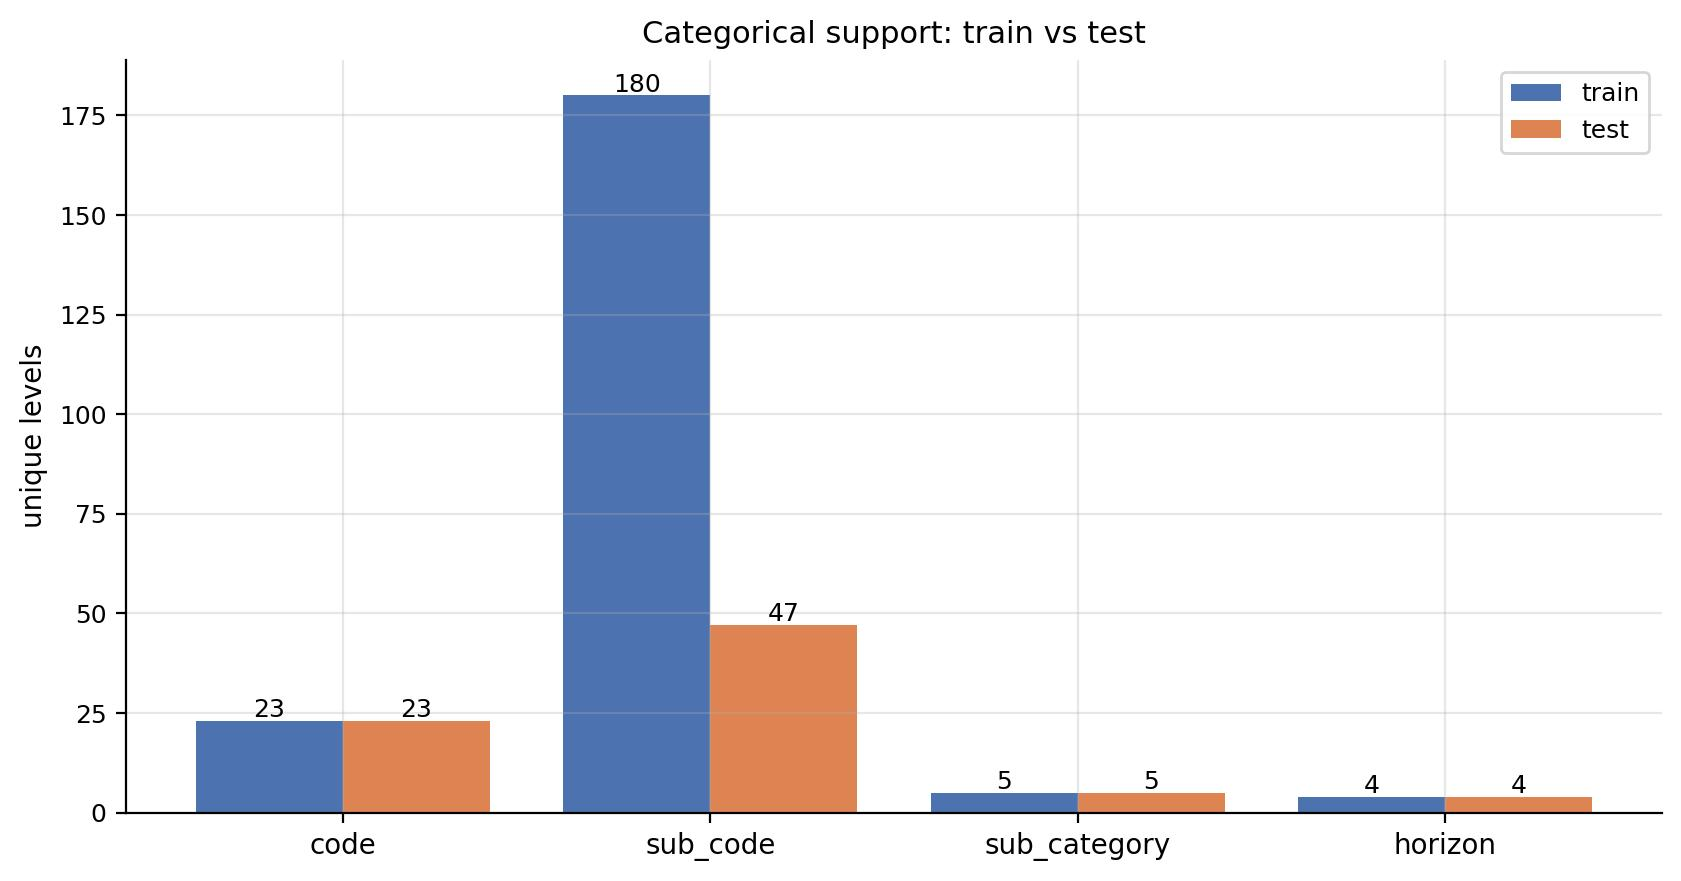
\includegraphics[width=0.85\linewidth]{figures/support_check.jpeg}
\caption{Comparison of categorical coverage between train and test sets, showing consistent schema but reduced sub\_code support in the test data.}
\label{fig:support_check}
\end{figure}

\subsection{The four horizons are coupled}

A naive reading of the schema would treat the four horizons of the same $(\mathtt{code},\mathtt{sub\_code},\mathtt{sub\_category})$ as four independent series, simply distinguished by an extra integer label. Two empirical facts in \cref{sec:eda} contradict this view:

\begin{enumerate}
  \item For approximately 1.21 million distinct $(\mathtt{code},\mathtt{sub\_code},\mathtt{sub\_category},\mathtt{ts\_index})$ tuples, all four horizons are simultaneously present (\cref{sec:multihorizon}).
  \item For the same triple, the target at horizon $k$ is closely approximated by the rolling sum of the $H=1$ target over the next $k$ steps:
  \[
    y^{H_k}_t \;\approx\; \sum_{i=0}^{k-1} y^{H_1}_{t+i}.
  \]
  We verify this on a stratified sample of 500 triples in \cref{sec:cumulation}, and find median Pearson correlations of 0.96, 0.94 and 0.91 at $k=3,10,25$ respectively.
\end{enumerate}

The practical consequence is that fitting four independent regressors per triple discards a strong constraint that the data construction itself imposes. We exploit this constraint in the H1-aggregation experiment scheduled for a later notebook.

\subsection{Chronological constraint}

The training partition runs over $\mathtt{ts\_index} \in [1, 3601]$ and the test partition over $[3602, 4376]$. Because test is a strict temporal suffix of train, any internal validation strategy must also be chronological, with all training points strictly preceding the validation points in time. Random or leave-one-series-out cross-validation would mix future information into earlier states and overstate generalisation.

We use a single canonical chronological partition throughout the project, fixed in the shared utilities at \texttt{cf.splits}:

\begin{itemize}
  \item \textbf{Train:} $\mathtt{ts\_index} \le 2880$.
  \item \textbf{Meta} (used only for fitting ensemble weights): $2880 < \mathtt{ts\_index} \le 3240$.
  \item \textbf{Holdout} (final scored window): $3240 < \mathtt{ts\_index} \le 3601$.
  \item \textbf{Test} ($\mathtt{ts\_index} \ge 3602$): unlabeled, used only for submission-style sanity checks.
\end{itemize}

The cutoff $\mathtt{ts\_index} = 2880$ matches the cutoff used in the midway report, preserving comparability with prior diagnostic figures. The meta/holdout boundary at 3240 places approximately one third of the post-cutoff window into the meta slice, leaving the remaining two thirds for final scoring.

\subsection{Eligibility for per-series studies}

Some classical model families (ARIMA, ARMA, MA, AR with order $\geq 2$) require a minimum training history. For per-series diagnostic studies we restrict attention to series that both cross the train/validation cutoff and have at least 120 training rows. There are 1{,}930 such \emph{eligible} series in the panel, roughly 5\% of the 36{,}923 total. Global pooled models and the H1-aggregation experiment use every row whose $\mathtt{ts\_index}$ falls inside the relevant split, so they are not constrained by per-series length.

\section{The Weighted Skill Score}
\label{sec:skill}

The competition is decided by a single scalar: the \emph{weighted skill score}. Because the rest of the project uses this metric for every model comparison, ensemble weight, and bootstrap interval, it deserves a dedicated section. We state the formula, give the intuitive reading, and note the two practical consequences that carry through every modelling decision.

\subsection{Definition}

Given truths $y_i$, predictions $\hat y_i$, and non-negative weights $w_i$ for $i = 1, \ldots, n$, the weighted skill score is
\begin{equation}
\label{eq:skill}
  \text{score}(y, \hat y; w) \;=\; \sqrt{\,1 \;-\; \mathrm{clip}_{[0,1]}\!\left( \dfrac{\sum_{i} w_i\,(y_i - \hat y_i)^2}{\sum_{i} w_i\,y_i^2} \right)\,}
\end{equation}
where $\mathrm{clip}_{[0,1]}(x) = \min(\max(x,0),1)$. The function returns 1 for a perfect prediction and 0 when the prediction is no better than the all-zero forecast.

\subsection{Intuitive meaning}

Strip away the symbols and the score answers a single question: \emph{how much of the weighted target ``energy'' is left unexplained by the prediction?}

The fraction inside the square root, $\sum w_i (y_i - \hat y_i)^2 \,/\, \sum w_i y_i^2$, is exactly that --- the unexplained share of weighted squared truth. It is zero when the prediction is perfect and one when the prediction is identically zero. The clip caps it at one so that no model can score worse than the trivial all-zero forecast, and the outer square root puts the result on a familiar correlation-like scale where 1 is excellent, 0 is no skill, and intermediate values read roughly the way a Pearson correlation of the same magnitude reads.

A few useful reference points:

\begin{itemize}
  \item \textbf{Skill $= 1$} --- perfect predictions on every weighted row.
  \item \textbf{Skill $= 0$} --- the model is no better than predicting zero. This is the natural ``did you learn anything'' threshold.
  \item \textbf{Skill $\approx 0.5$} --- roughly three quarters of the weighted target energy is still unexplained. In feel, this is comparable to a Pearson correlation of $0.5$: a real but modest signal.
  \item \textbf{Skill $\approx 0.95$} --- only ten percent of energy unexplained. Strong, near the practical ceiling for a competitive entry.
\end{itemize}

The reason the metric is built around \emph{weighted} energy rather than raw error is that hedge-fund-style panels have wildly different target scales across instruments. Dividing by $\sum w_i y_i^2$ neutralises that scale: a 1\% relative error on a low-volatility row and a 1\% relative error on a high-volatility row contribute proportionally to the score. The weights $w_i$ themselves let the organiser encode importance and in our panel those weights are extraordinarily concentrated, so the score is effectively decided by how well the model fits a small set of high-weight rows.

\subsection{Practical consequences for this project}

\Cref{eq:skill} is implemented once in the shared utility \texttt{cf.metrics.weighted\_skill\_score} and used by every later notebook for both model selection and final scoring. The function \texttt{cf.metrics.bootstrap\_skill} returns 95\% confidence intervals by row resampling; we report bootstrap intervals alongside every leaderboard number to avoid declaring winners that are within sampling noise of each other.

Two structural observations carry through to every subsequent modelling decision:

\begin{itemize}
  \item \textbf{High-weight rows decide the leaderboard.} Because approximately 64\% of weight sits in the top 1\% of rows (\cref{sec:weight_dist}), the score is essentially a measure of how well the model predicts those few rows. We must therefore train with sample weights, not just evaluate with them.
  \item \textbf{Plain RMSE will lie.} A model that improves average behaviour at the cost of a small degradation on a high-weight row can lose to a simpler model. We never report unweighted RMSE as a primary headline number.
\end{itemize}

\section{Data Pre-processing and Exploratory Analysis}
\label{sec:eda}

This section reports the exploratory analysis of the panel before any modelling. The aim is twofold. First, to establish the basic statistical shape of the data so that later modelling choices can be motivated rather than guessed. Second, to surface three structural findings about the panel --- multi-horizon coupling, the cumulation hypothesis, and per-horizon weight dominance --- that the midway report did not document but that materially change the modelling space. All numerical results below are produced by notebook \texttt{00\_data\_structure.ipynb} and the corresponding figures are saved as both PNG and PDF assets.

\subsection{Schema, panel scale, and train--test comparability}
\label{sec:eda:schema}

The training panel contains 5{,}337{,}414 rows, organised by 23 distinct \texttt{code} values, 180 distinct \texttt{sub\_code} values, and 5 \texttt{sub\_category} values across 4 horizons. The integer time index $\mathtt{ts\_index}$ runs over the contiguous range $[1, 3601]$. The test partition continues from $\mathtt{ts\_index} = 3602$ to 4376 with 1{,}447{,}107 rows, so test is a strict temporal suffix of train. Treating the 4-tuple $(\mathtt{code},\mathtt{sub\_code},\mathtt{sub\_category},\mathtt{horizon})$ as the natural series identifier yields 36{,}923 distinct series.

The only columns present in train but not in test are $y_{\text{target}}$ and $\mathtt{weight}$, as expected. Every category level seen in test exists in train, so there is no cold-start schema issue. The sub-code support narrows from 180 in train to 47 in test --- a coverage shift rather than a schema mismatch.

\subsection{Missing values}
\label{sec:eda:missing}

Missingness is computed on a 500{,}000-row stratified sample to keep memory in check. Of the 86 anonymised features, 48 contain at least one missing value, but the maximum missing rate across all columns is approximately 12.5\%. \Cref{fig:missingness} shows the top fifteen offenders.

\begin{figure}[H]
\centering
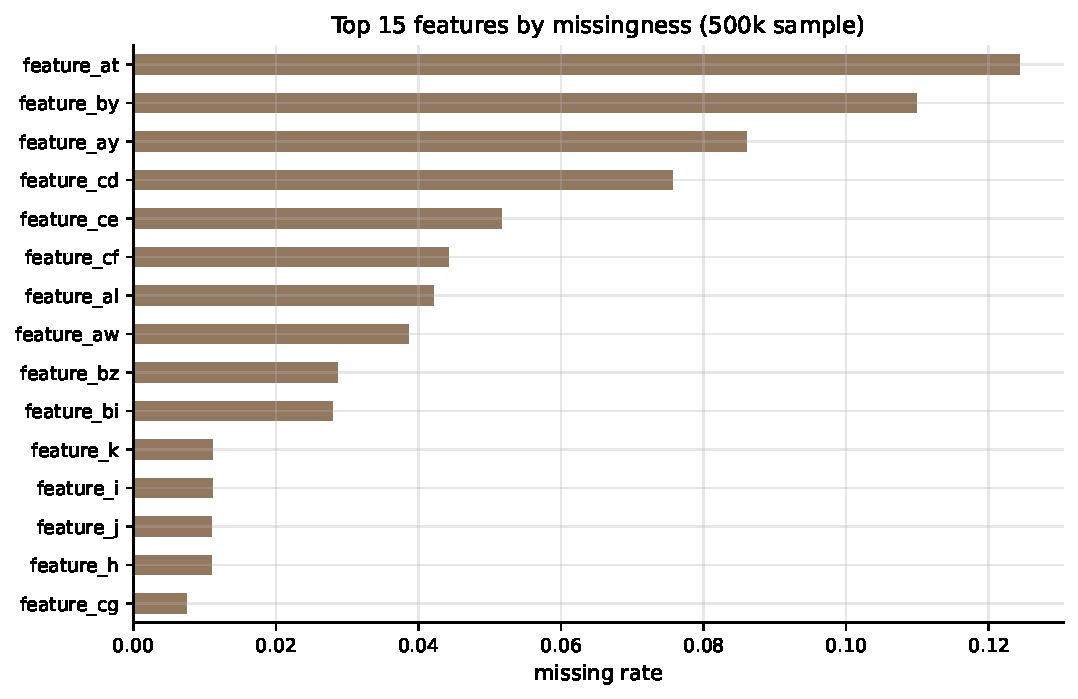
\includegraphics[width=0.85\linewidth]{00_missingness_top15}
\caption{Top fifteen features by missingness, on a 500{,}000-row stratified sample of train. The maximum missing rate is approximately 12.5\%, low enough that median imputation inside a fold is sufficient and there is no need to drop columns or use complex imputers.}
\label{fig:missingness}
\end{figure}

\paragraph{Reading.} Missing rates are bounded; within-fold median imputation suffices. No separate imputation strategy is developed.

\subsection{Target distribution}
\label{sec:eda:target}

The target $y_{\text{target}}$ is centred very close to zero (median $-0.0006$, IQR $\pm 0.05$), but has extremely heavy tails. The 1\% and 99\% quantiles sit at approximately $-82.8$ and $+62.9$ respectively, while the full range runs from approximately $-2202$ to $+2314$.

\begin{figure}[H]
\centering
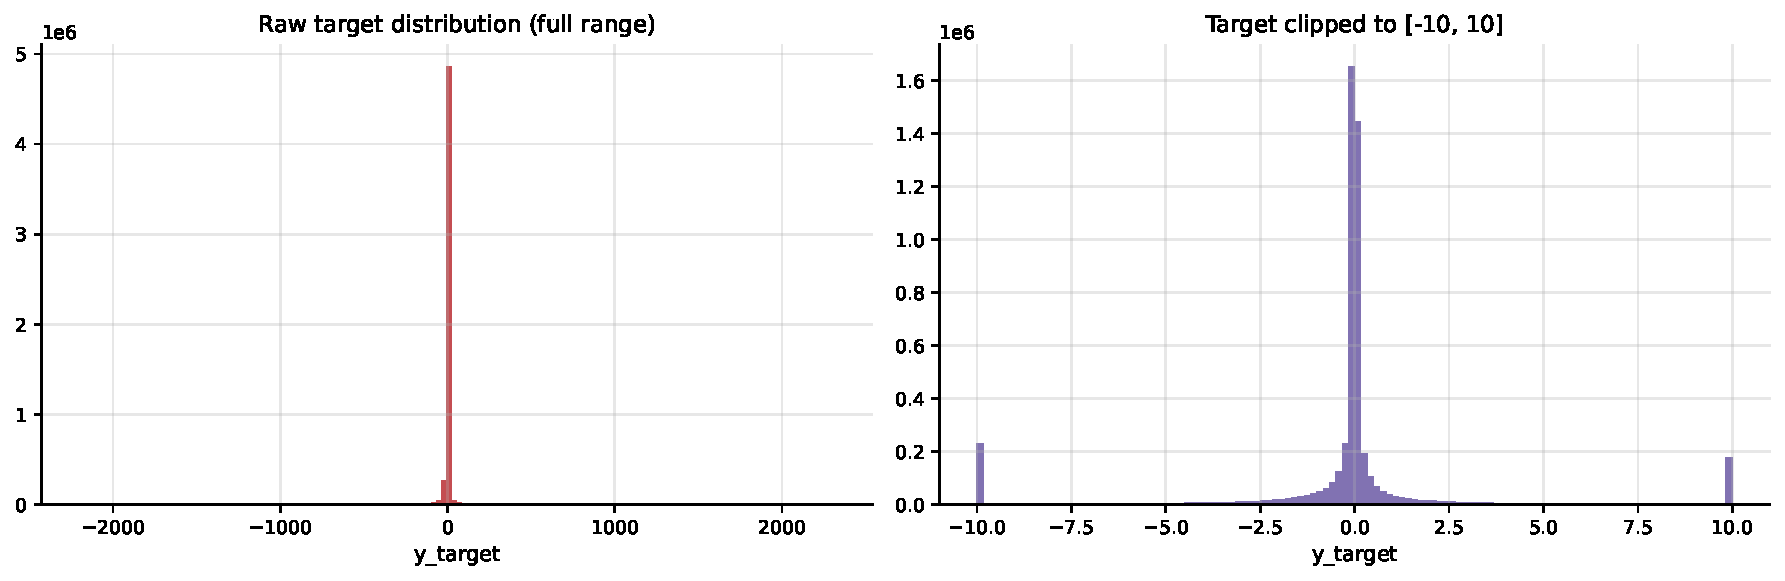
\includegraphics[width=0.95\linewidth]{00_target_distribution}
\caption{Raw target distribution (left) and the same distribution clipped to $[-10, 10]$ (right). Most of the mass concentrates near zero, with rare extreme tails up to the order of $\pm 2200$.}
\label{fig:target_dist}
\end{figure}

\paragraph{Reading.} The shape disqualifies plain unweighted MSE as a sensible loss. Tails are real outcomes, not corruption, so we cannot simply clip them; combined with the weighting scheme below, this is the central methodological constraint.

\subsection{Weight distribution and metric concentration}
\label{sec:weight_dist}

The competition weights are extraordinarily skewed. The median weight is $1{,}699$, while the maximum is $1.39 \times 10^{13}$. \Cref{fig:weight_dist} shows the weight distribution clipped at the 99th percentile (left) and the cumulative-share Lorenz-style curve (right). The top 1\% of rows carry 64.2\% of total weight; the top 5\% carry 92.6\%; the top 10\% carry 98.3\%.

\begin{figure}[H]
\centering
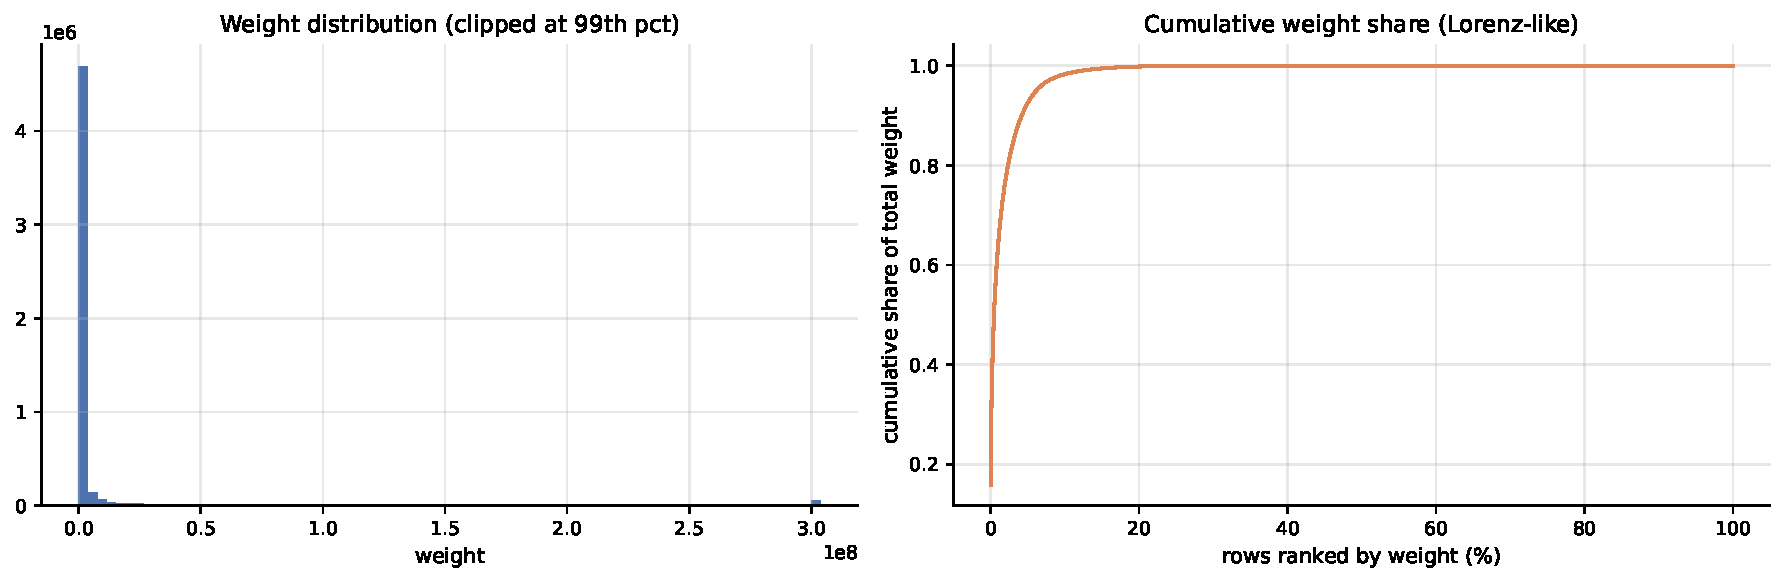
\includegraphics[width=0.95\linewidth]{00_weight_distribution}
\caption{Weight distribution clipped at the 99th percentile (left) and cumulative share of total weight ranked by weight (right). Approximately 64\% of total weight is concentrated in the top 1\% of rows; 92\% in the top 5\%.}
\label{fig:weight_dist}
\end{figure}

\paragraph{Reading.} Unweighted evaluation describes a different competition. The weighted skill score (\cref{sec:skill}) is our only headline metric, and a model that accurately predicts the top one percent of rows has more leverage on the leaderboard than a uniformly mediocre one.

\subsection{Series coverage and split feasibility}
\label{sec:eda:coverage}

Not every series has enough history to support time-based validation. \Cref{fig:series_length} shows the distribution of per-series lengths. Out of 36{,}923 distinct series, only 1{,}930 (approximately 5\%) cleanly cross the train/validation cutoff at $\mathtt{ts\_index} = 2880$. Many series end before the cutoff, contributing zero validation rows.

\begin{figure}[H]
\centering
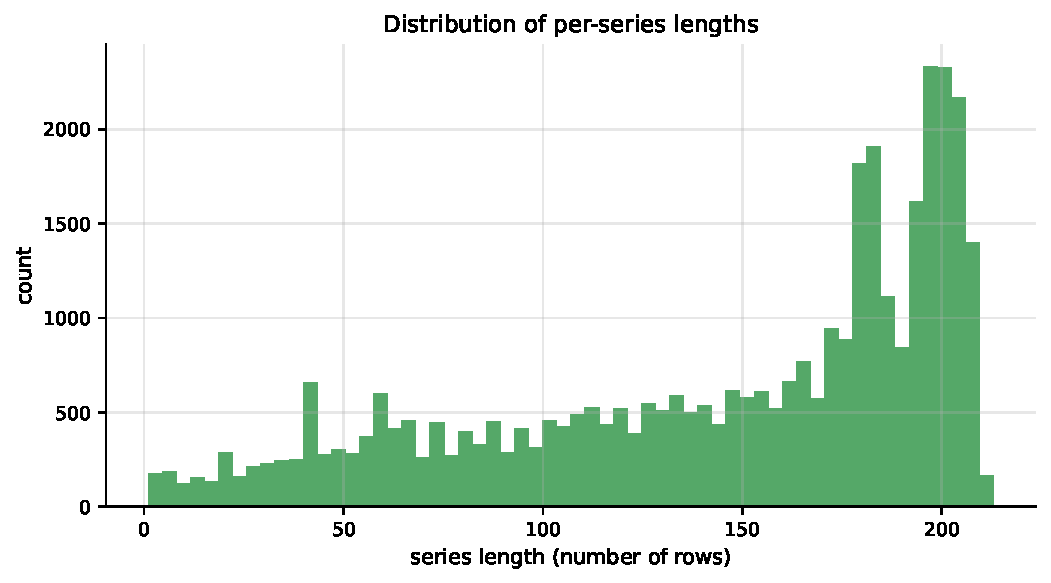
\includegraphics[width=0.85\linewidth]{00_series_length_distribution}
\caption{Distribution of per-series lengths. Most series are short, and the tail of long series carries the structural signal that classical fits can exploit.}
\label{fig:series_length}
\end{figure}

\paragraph{Reading.} Per-series classical fitting is feasible only on the eligible subset (cross the cutoff with at least 120 training rows). Global pooled models are not length-constrained --- one reason the comparison between local classical and global ML approaches is not perfectly apples-to-apples.

\subsection{Representative-series selection}
\label{sec:eda:repseries}

For every per-series figure in this project we plot the same four series. They are selected with explicit reasons rather than at random, in order to span four distinct stress regimes: long history, large weight, high variability, and near-flat behaviour. \Cref{tab:representative} lists the four chosen series. They match the selection used in the midway report, preserving visual continuity.

\begin{table}[H]
\centering
\caption{Four representative series chosen for per-series studies. Each series probes a different regime of the panel.}
\label{tab:representative}
\begin{tabular}{l l l c}
\toprule
Reason & Series key (code/sub\_code) & Horizon & Length \\
\midrule
Longest history       & X9BZ68VQ / OYJGNSQK / DPPUO5X2 & 1  & 212 \\
Highest total weight  & SJZP0OVU / OYJGNSQK / NQ58FVQM & 25 & 156 \\
Most volatile         & W4S29LF4 / KL66VIS3 / PHHHVYZI & 25 & 162 \\
Most stable           & SJZP0OVU / OYJGNSQK / NQ58FVQM & 1  & 170 \\
\bottomrule
\end{tabular}
\end{table}

\Cref{fig:rep_series_raw} shows the raw $y_{\text{target}}$ trajectory of each chosen series with the train/validation cutoff marked. The four panels look profoundly different: the most-volatile series swings between $-500$ and $+500$, while the most-stable series occupies a numerical range narrower than $0.001$.

\begin{figure}[H]
\centering
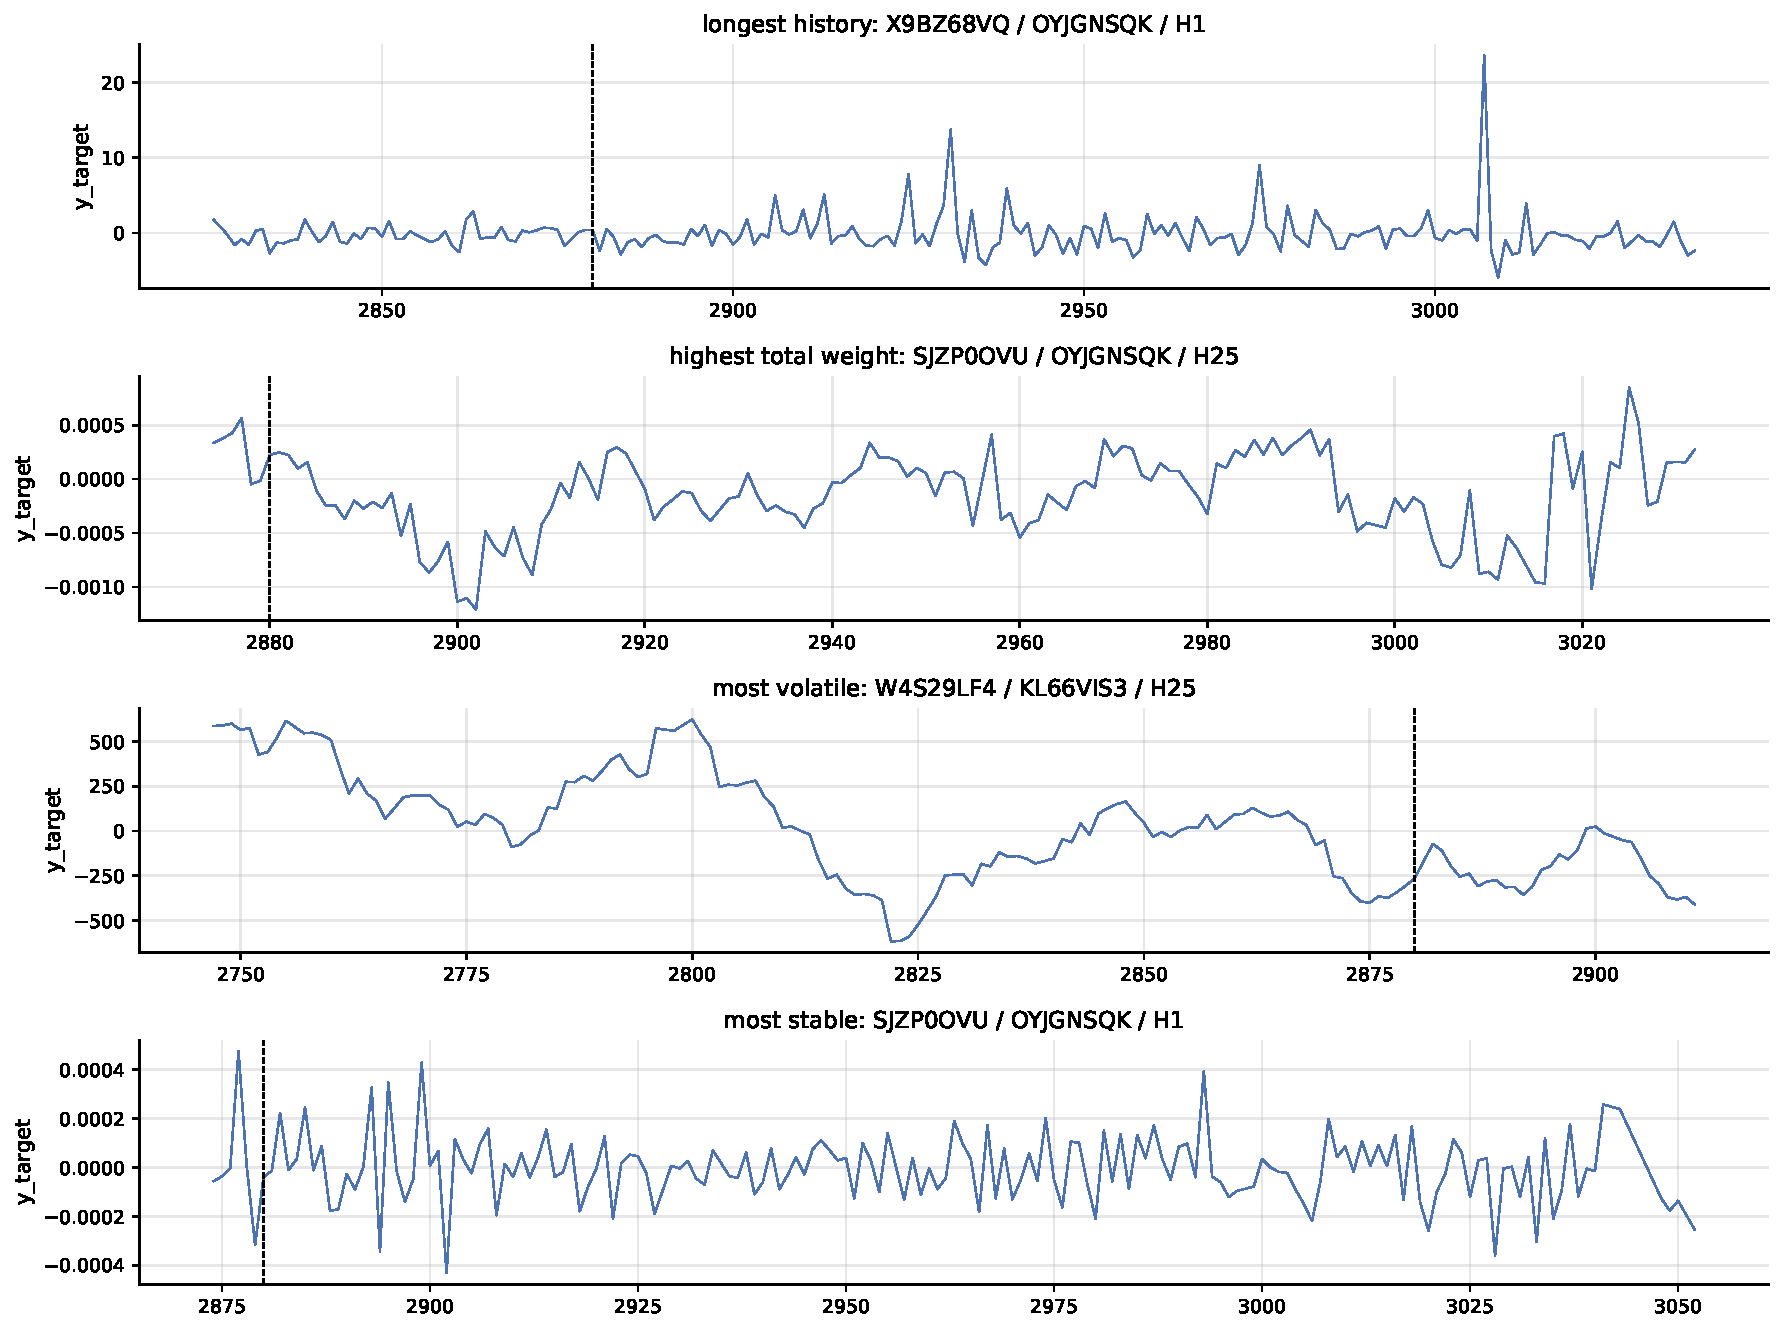
\includegraphics[width=0.95\linewidth]{00_representative_series_raw}
\caption{Raw $y_{\text{target}}$ for the four chosen representative series. The dashed vertical line marks $\mathtt{ts\_index} = 2880$, the train/validation cutoff. The four panels span the four stress regimes that any model has to handle.}
\label{fig:rep_series_raw}
\end{figure}

\paragraph{Reading.} A one-size-fits-all model will struggle: the most-stable series is essentially numerical noise, while the most-volatile series has obvious cyclical structure. Forecast performance across these four panels is one of the cleanest diagnostics for whether a model family generalises or only fits one regime.

\subsection{Stationarity diagnostics}
\label{sec:eda:stationarity}

Classical ARIMA-family forecasting assumes stationarity, or stationarity-after-differencing. We therefore run the Augmented Dickey--Fuller test on a stratified sample of 200 eligible series. The ADF test takes the null hypothesis that the series has a unit root (non-stationary); we reject at the 5\% level when the $p$-value is below $0.05$. \Cref{fig:adf} summarises the results.

\begin{figure}[H]
\centering
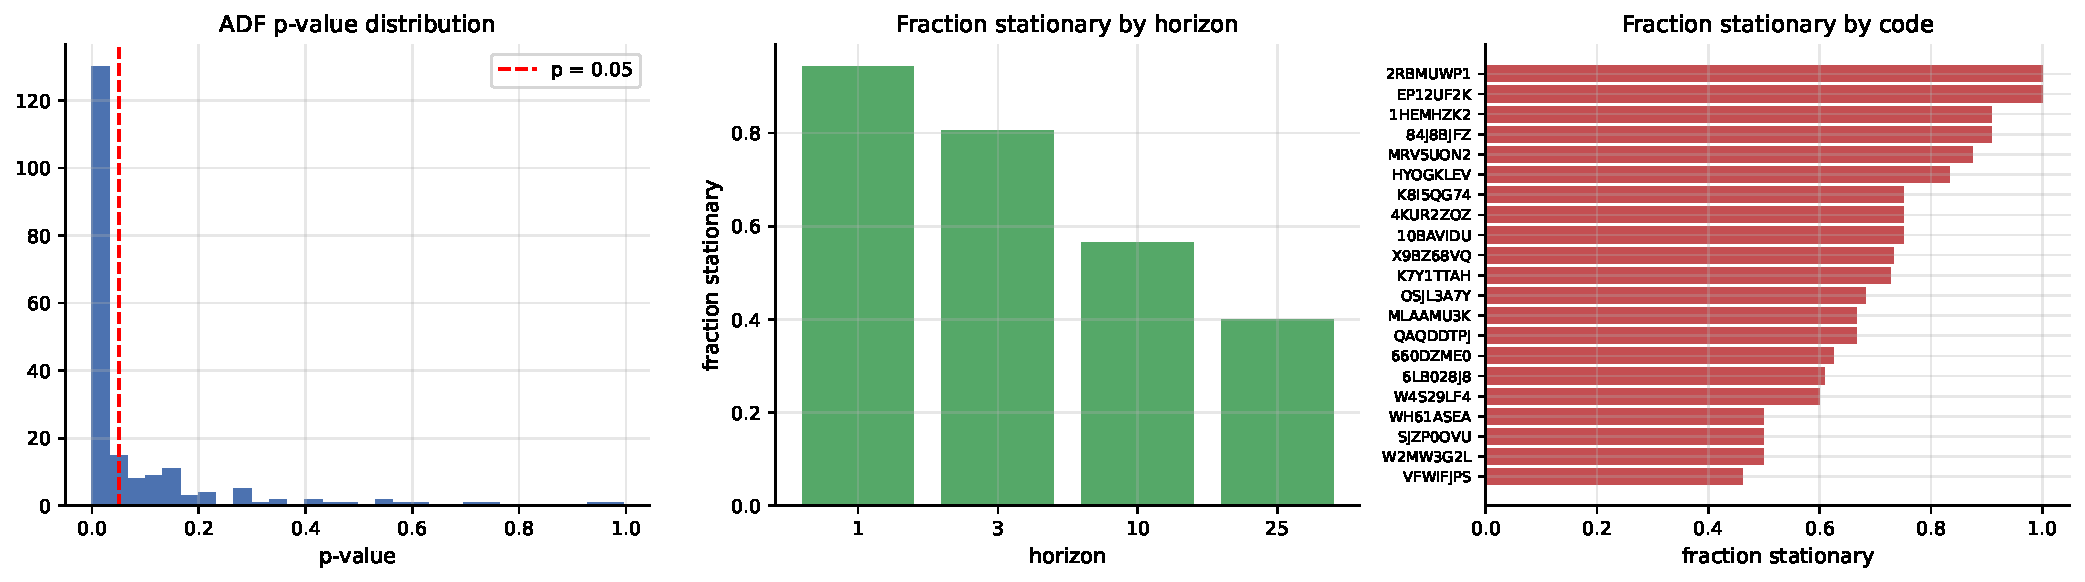
\includegraphics[width=0.95\linewidth]{00_adf_results}
\caption{ADF results on 200 sampled eligible series. Left: $p$-value distribution with the $0.05$ threshold marked. Centre: fraction stationary by horizon. Right: fraction stationary by code.}
\label{fig:adf}
\end{figure}

Approximately 70.5\% of sampled series reject the unit-root null at the 5\% level. The picture is more nuanced when broken down by horizon: H1 series are more often stationary than longer-horizon cumulative series, which is consistent with the multi-horizon coupling we will document in \cref{sec:cumulation}.

ADF and KPSS have opposite null hypotheses, so running both gives a more honest joint verdict: ADF takes non-stationarity as the null, while KPSS takes stationarity as the null. We classify a series as \emph{stationary} when ADF rejects and KPSS does not, as \emph{unit root} when ADF fails to reject and KPSS rejects, and as \emph{inconclusive} otherwise. \Cref{fig:adf_kpss} reports the joint distribution.

\begin{figure}[H]
\centering
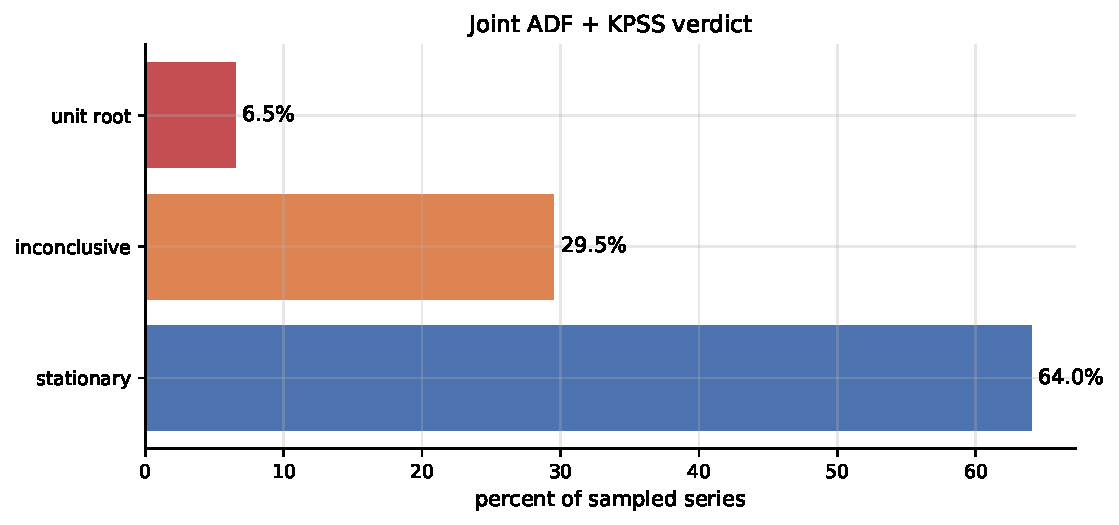
\includegraphics[width=0.7\linewidth]{00_adf_kpss_joint}
\caption{Joint ADF $+$ KPSS verdict on 200 sampled series. Stationary 64.0\%, inconclusive 29.5\%, unit root 6.5\%.}
\label{fig:adf_kpss}
\end{figure}

The stationary share dominates, but the inconclusive bucket is large enough that one-size-fits-all claims about raw levels would be unsafe. We need a repair step (differencing) for the unit-root and inconclusive cases.

\Cref{fig:differencing} re-runs the ADF test on the first-differenced series. The stationary share rises from 70.5\% on raw levels to 98.5\% after differencing.

\begin{figure}[H]
\centering
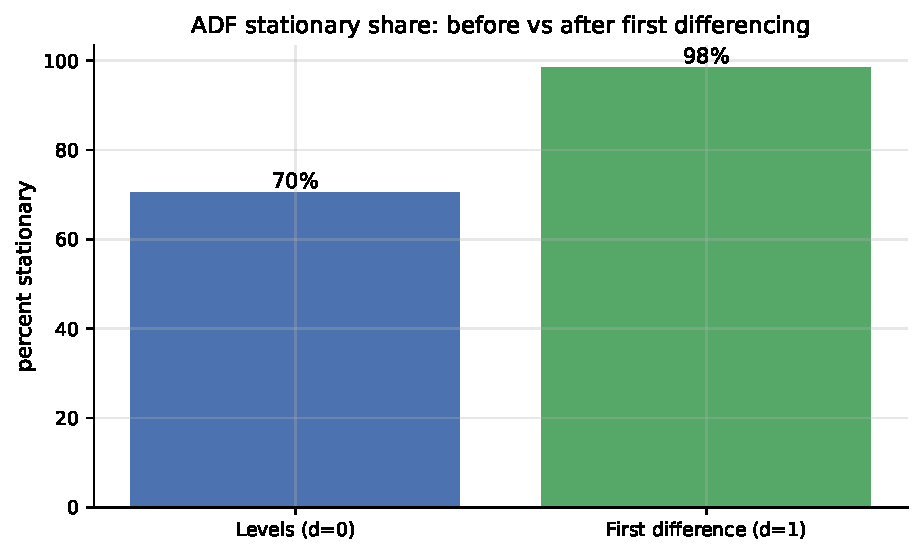
\includegraphics[width=0.7\linewidth]{00_first_differencing_share}
\caption{ADF stationary share at the 5\% level: levels (left, $d=0$) versus first differences (right, $d=1$). Differencing pushes the share to nearly 100\%.}
\label{fig:differencing}
\end{figure}

\paragraph{Reading.} The diagnostic chain motivates ARIMA with $d=1$ as the default for the classical study and justifies engineered differenced features for global ML models. The 98.5\% post-difference stationarity also bears on the cumulation finding in \cref{sec:cumulation}: differencing a higher-horizon target partially inverts the rolling-sum construction back into the H1 process.

\subsection{Visual stationarity --- rolling statistics}
\label{sec:eda:rolling}

Statistical tests can disagree on short or noisy series, so a rolling-window view is a useful visual check. \Cref{fig:rolling_raw} shows a 24-step rolling mean and rolling standard deviation on the raw four representative series. The most-volatile series shows clear drift in level and bulging variance; the longest-history series drifts upward; the high-weight and most-stable series occupy near-flat ranges where the rolling mean barely moves.

\begin{figure}[H]
\centering
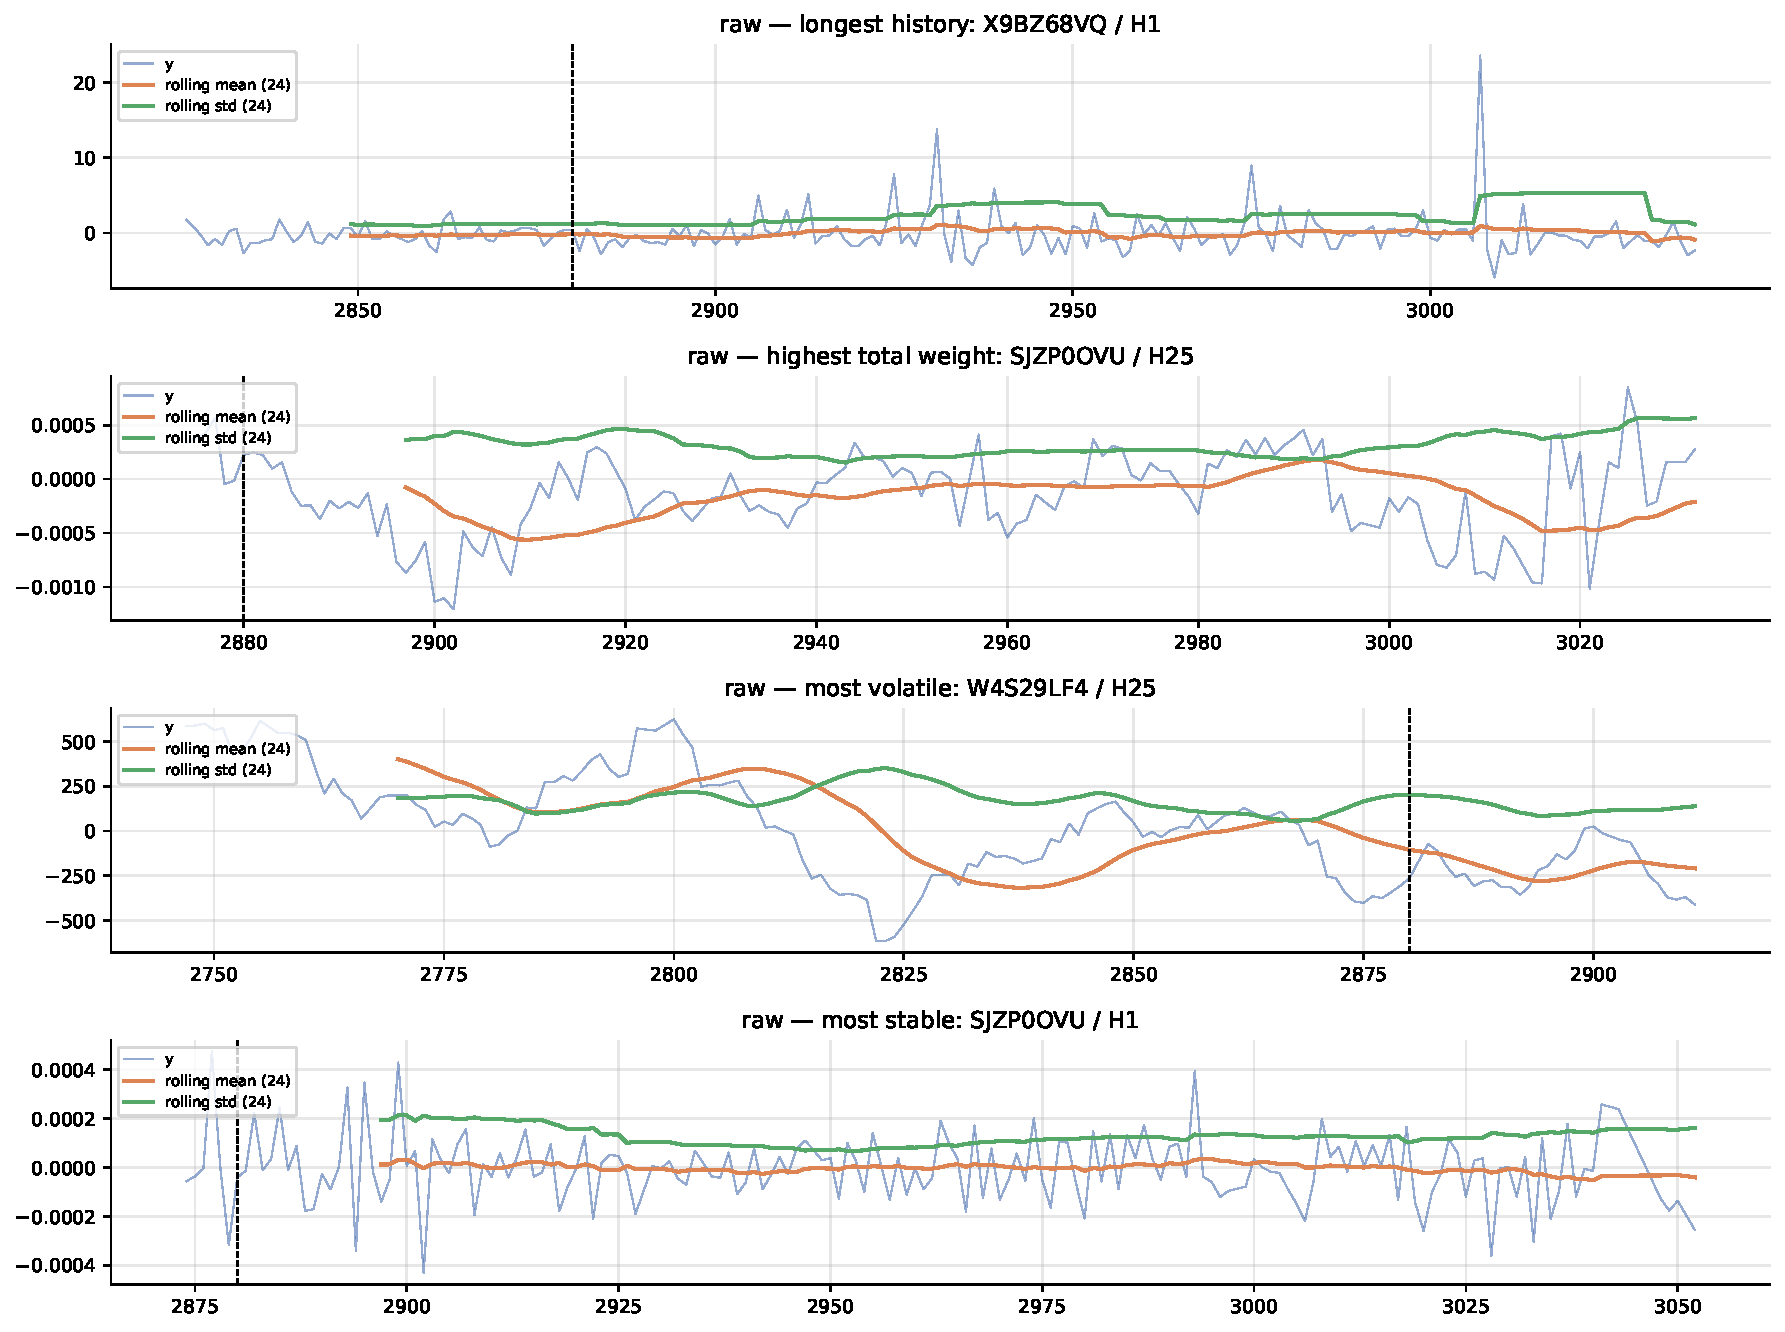
\includegraphics[width=0.95\linewidth]{00_rolling_raw}
\caption{Rolling mean and rolling standard deviation (window = 24) on the raw four representative series. The most-volatile series shows clear drift in level and bulging variance.}
\label{fig:rolling_raw}
\end{figure}

\Cref{fig:rolling_diff} repeats the same diagnostic on the first-differenced versions of the same series. The rolling means now hug zero and the rolling standard deviations flatten across the cutoff, visually confirming the statistical jump from the previous subsection.

\begin{figure}[H]
\centering
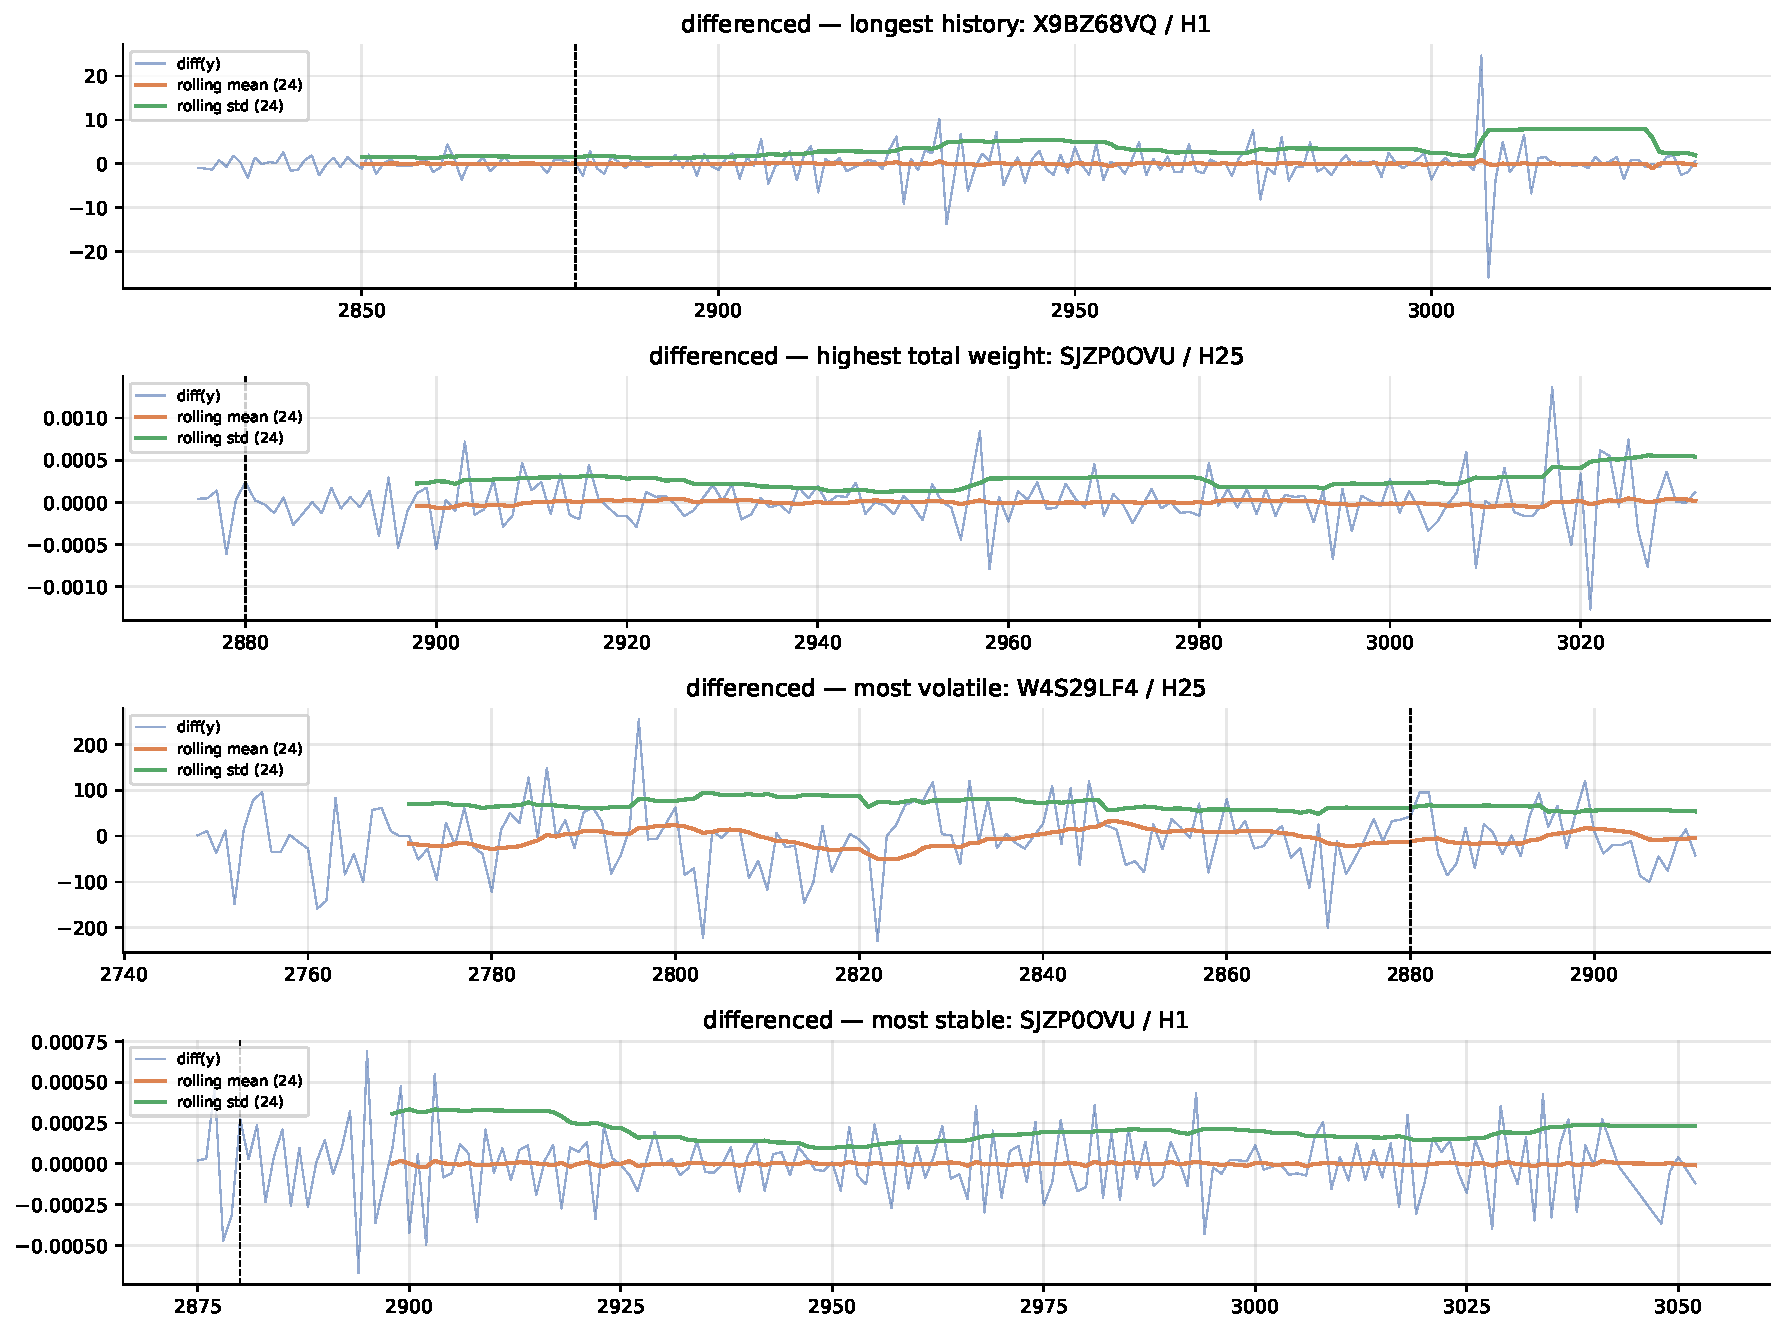
\includegraphics[width=0.95\linewidth]{00_rolling_differenced}
\caption{Rolling mean and rolling standard deviation (window = 24) on the first-differenced four representative series. The mean oscillates close to zero and the variance is stable, consistent with stationarity.}
\label{fig:rolling_diff}
\end{figure}

\paragraph{Reading.} Differenced series behave like the white-noise regime we want before fitting a differenced classical model.

\subsection{Lag Structure: ACF and PACF}
\label{sec:eda:acf_pacf}

Understanding the temporal dependence structure of the series is essential for selecting appropriate forecasting models. We therefore analyse both the autocorrelation function (ACF) and partial autocorrelation function (PACF), first on a representative anchor series and then at the panel level.

\subsubsection{Anchor-series correlograms}

We begin with the longest-history representative series, which provides sufficient data to expose meaningful lag structure. The ACF measures correlation between the series and its lagged values, while the PACF isolates the direct contribution of each lag after controlling for shorter lags.

\begin{figure}[H]
\centering
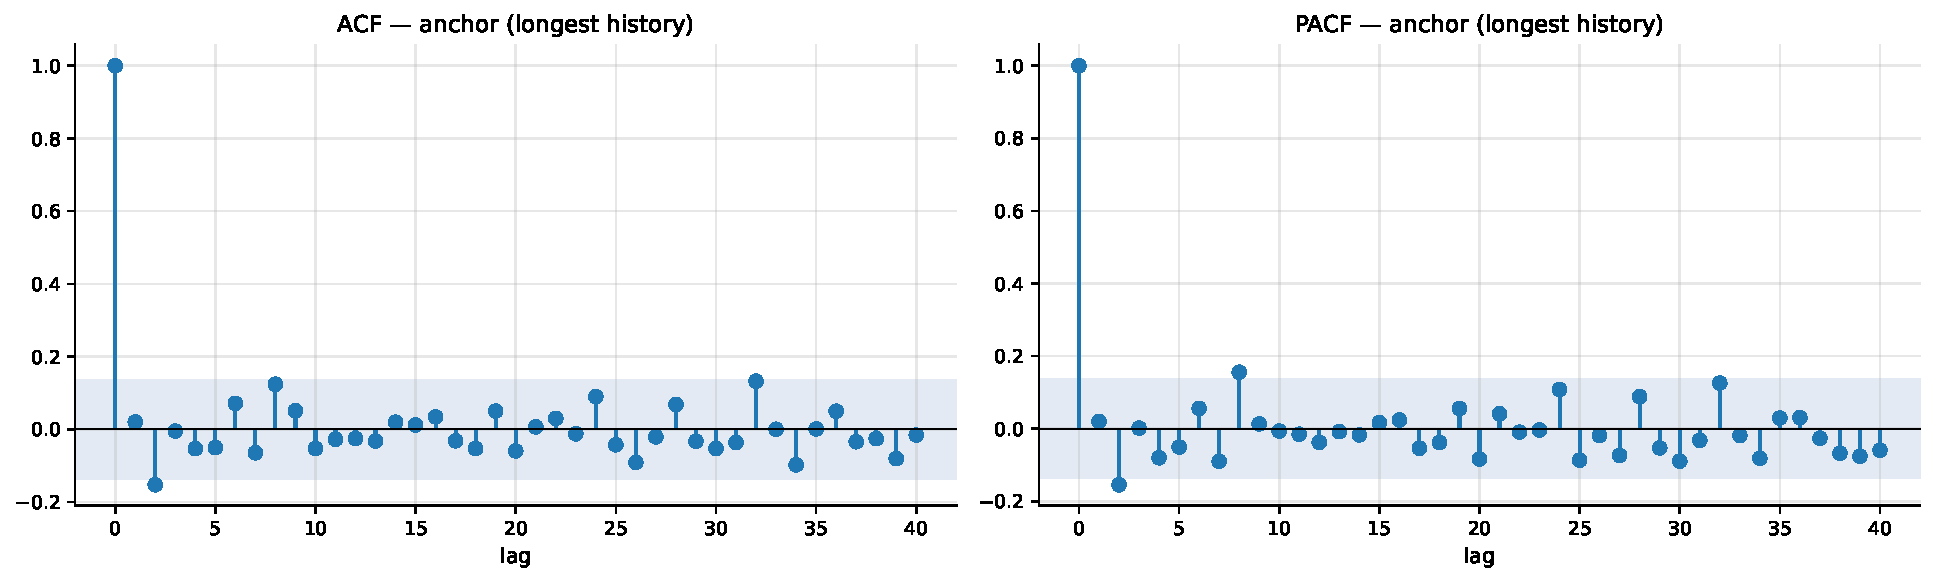
\includegraphics[width=0.95\linewidth]{00_acf_pacf_anchor}
\caption{ACF (left) and PACF (right) for the longest-history representative series. The ACF shows gradual decay, while the PACF exhibits a sharp cutoff after the first few lags, suggesting a low-order autoregressive structure.}
\label{fig:acf_pacf_anchor}
\end{figure}

\paragraph{Reading.}
The ACF shows a smooth decay rather than a sharp cutoff, indicating persistence but not strong periodicity. The PACF exhibits significant spikes at the first few lags (typically lag 1--3), after which contributions become negligible. This pattern is consistent with short-memory autoregressive dynamics rather than long-range dependence or seasonal structure.

\subsubsection{Panel-level aggregation}

While anchor-series analysis is informative, relying on a single trajectory risks overfitting conclusions to one series. To obtain a more robust view, we aggregate the absolute ACF and PACF values across a stratified sample of 200 eligible series.

\begin{figure}[H]
\centering
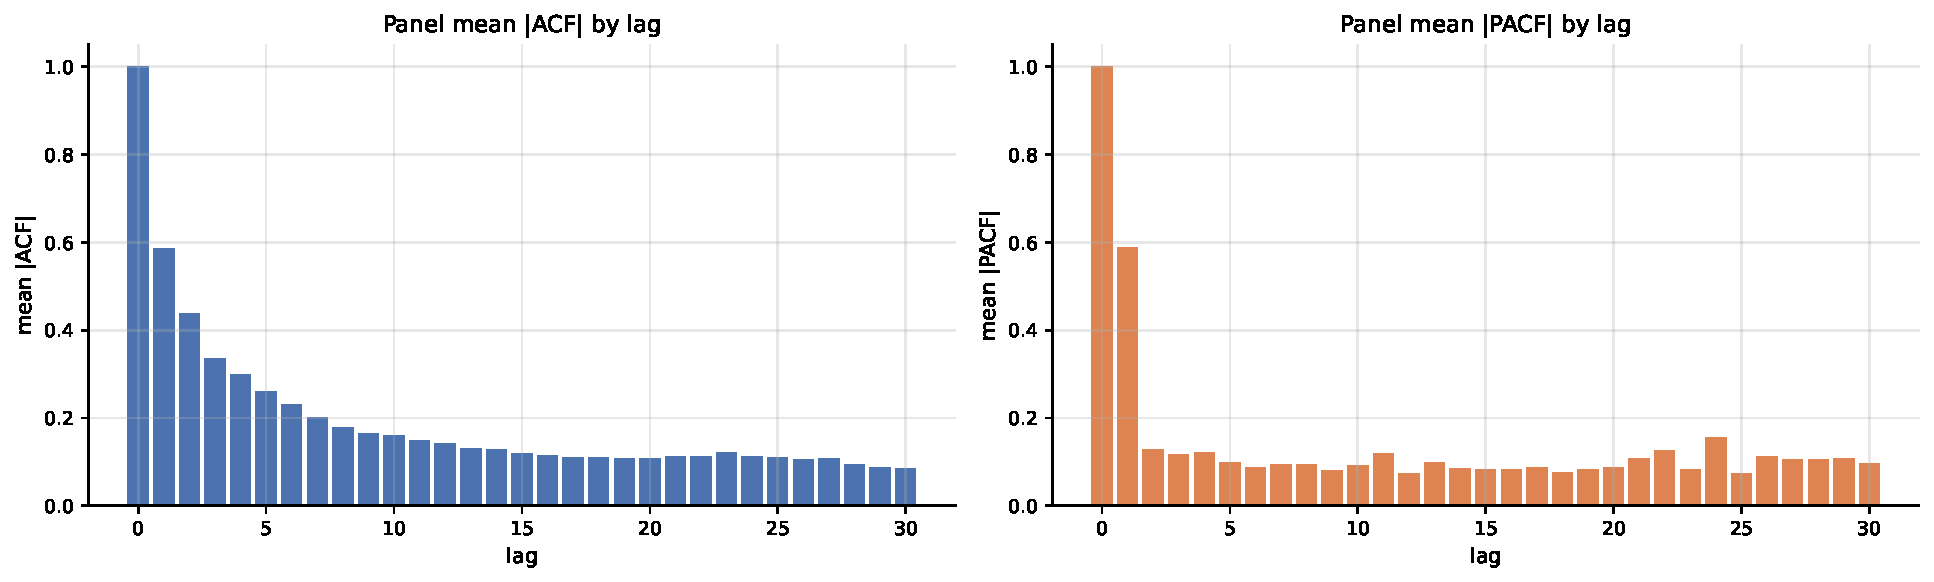
\includegraphics[width=0.95\linewidth]{00_acf_pacf_panel}
\caption{Panel-level mean absolute ACF (left) and PACF (right) across 200 sampled series. Low-order lags dominate, with rapid decay beyond lag 3--5 and no clear seasonal peaks.}
\label{fig:acf_pacf_panel}
\end{figure}

\paragraph{Reading.}
The aggregated correlograms confirm that the panel is dominated by short-memory dynamics. Lags 1--3 consistently carry the strongest signal, with contributions decaying rapidly thereafter. There are no pronounced periodic spikes, indicating the absence of strong seasonal structure across the panel.

\subsubsection{Modelling implications}

The combined anchor and panel-level diagnostics lead to three practical conclusions:

\begin{itemize}
    \item \textbf{Low-order lag structure dominates.} Models should prioritise short lags (1, 2, 3, and optionally 5 or 10), as higher-order dependencies are weak and inconsistent.
    
    \item \textbf{No strong seasonality.} The absence of clear periodic patterns suggests that seasonal models or explicit seasonal features are unlikely to provide significant gains.
    
    \item \textbf{Support for ARIMA-type models.} The observed ACF/PACF patterns are consistent with low-order AR or ARMA processes after appropriate differencing, reinforcing the earlier stationarity diagnostics.
\end{itemize}

Overall, the correlogram analysis supports a modelling strategy focused on short-memory dynamics rather than complex seasonal or long-range structures.

\subsection{STL Decomposition}
\label{sec:eda:stl}

To investigate the presence of seasonal structure in the panel, we apply Seasonal-Trend decomposition using LOESS (STL) to one of the representative series. We focus on the \emph{most-stable} series, as its low variance makes any extracted structure easier to interpret and attribute.

\subsubsection{Motivation}

STL decomposes a time series into three additive components:
\begin{equation}
y_t = T_t + S_t + R_t,
\end{equation}
where $T_t$ is the trend component, $S_t$ is the seasonal component, and $R_t$ is the residual.

However, STL requires a fixed seasonal period as input. Since the dataset is anonymized and no domain-driven periodicity is available, the period must be inferred from the data.

\subsubsection{ACF-based period selection}
\label{sec:eda:stl_period}

We estimate the seasonal period using the sample autocorrelation function (ACF). The intuition is that if the series exhibits periodic behaviour with period $p$, then the autocorrelation at lag $p$ should be relatively large.

Given a time series $\{y_t\}_{t=1}^{T}$, we compute the empirical ACF:
\begin{equation}
\rho(k) = \frac{\sum_{t=k+1}^{T} (y_t - \bar{y})(y_{t-k} - \bar{y})}{\sum_{t=1}^{T} (y_t - \bar{y})^2}, \quad k = 0, 1, \dots, L,
\end{equation}
with $L = 100$.

The period selection follows a heuristic procedure:

\begin{enumerate}
    \item Compute $\rho(k)$ for $k = 0, 1, \dots, L$.
    \item Set $\rho(0) = 0$ to ignore the trivial maximum.
    \item Restrict attention to lags $k \geq 2$ to avoid degenerate short-lag effects.
    \item Identify the top candidate lags with highest autocorrelation values.
    \item Select the lag $p$ with the largest autocorrelation:
    \begin{equation}
        p = \arg\max_{k \in \mathcal{K}} \rho(k),
    \end{equation}
    where $\mathcal{K}$ denotes the set of candidate lags.
\end{enumerate}

Applying this procedure to the most-stable series yields:
\[
p = 8.
\]

\paragraph{Interpretation.}
The detected period corresponds to the strongest repeating lag in the autocorrelation structure. However, consistent with earlier ACF/PACF diagnostics (\cref{sec:eda:acf_pacf}), the autocorrelation does not exhibit sharp periodic peaks. Instead, multiple short lags have comparable magnitudes, indicating that the selected period should be interpreted as the strongest among weak candidates rather than evidence of a dominant seasonal cycle.

\subsubsection{STL decomposition}

\begin{figure}[H]
\centering
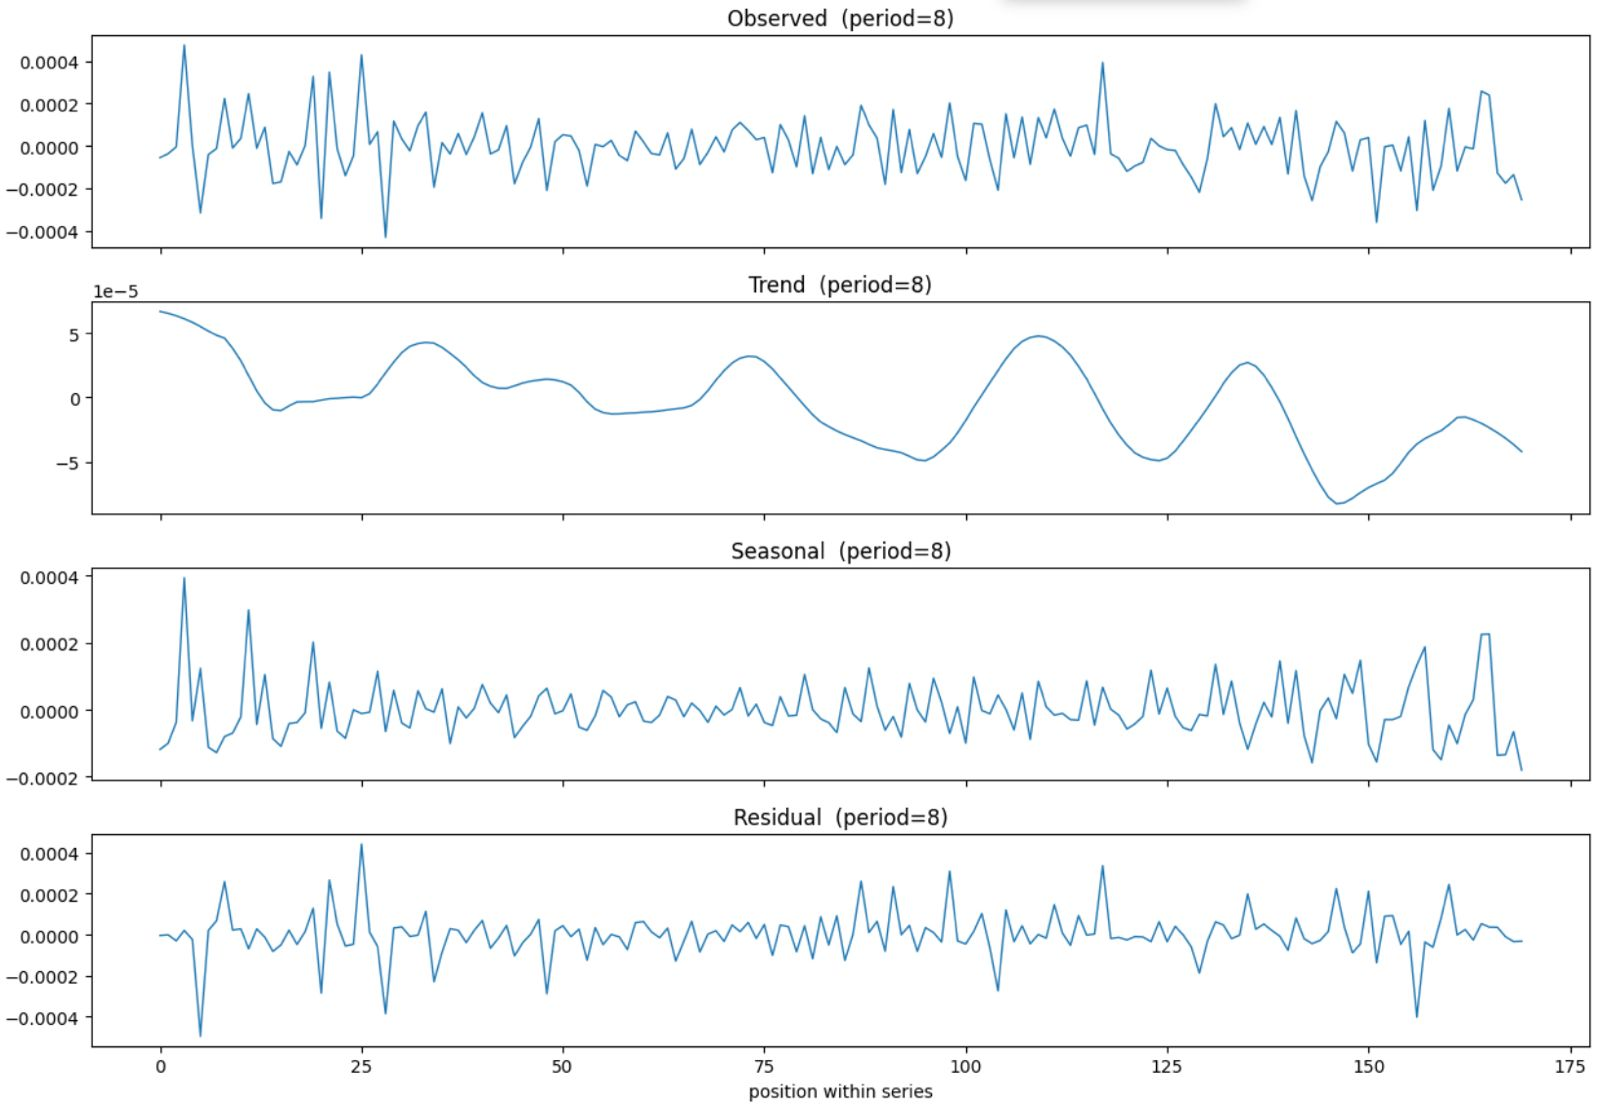
\includegraphics[width=0.95\linewidth]{00_stl_most_stable_p8}
\caption{STL decomposition of the most-stable representative series with selected period $p = 8$. The panels show the observed series (top), trend, seasonal, and residual components.}
\label{fig:stl_stable}
\end{figure}

\subsubsection{Reading}

Several observations follow from \cref{fig:stl_stable}:

\begin{itemize}
    \item \textbf{Observed series:} The signal fluctuates within a very narrow range, consistent with the definition of the most-stable series. No clear periodic structure is visually apparent.
    
    \item \textbf{Trend component:} The trend is smooth and low-amplitude, capturing slow drift rather than meaningful structural change. Due to the small scale of the series, even minor fluctuations appear visually pronounced.
    
    \item \textbf{Seasonal component:} The seasonal panel exhibits oscillatory behaviour at period $p=8$, but its magnitude is comparable to the noise level. The pattern aligns closely with short-lag autocorrelation rather than a true repeating seasonal cycle.
    
    \item \textbf{Residual component:} The residual captures irregular fluctuations and occasional spikes. For this near-flat series, most variation is effectively absorbed into the residual.
\end{itemize}

\subsubsection{Interpretation}

The STL decomposition does not provide evidence of genuine seasonality in the most-stable series. Instead, the apparent seasonal component arises from short-memory autocorrelation that is redistributed by the STL procedure when a short period is imposed.

This finding is consistent with earlier diagnostics:
\begin{itemize}
    \item The panel-level ACF shows rapid decay and dominance of low-order lags.
    \item The periodogram analysis does not reveal strong spectral peaks.
\end{itemize}

Taken together, these results indicate that the panel is primarily driven by short-memory dynamics rather than periodic structure.

\subsubsection{Implications for modelling}

The absence of meaningful seasonality has direct consequences for model design:

\begin{itemize}
    \item \textbf{Seasonal models are not prioritised.} There is no strong evidence supporting the use of seasonal ARIMA or explicit seasonal features.
    
    \item \textbf{Lag-based features are more relevant.} Short lags (e.g., 1--3, 5, 10) capture most of the temporal dependence.
    
    \item \textbf{Focus on stationarity and differencing.} Transformations that stabilise the series (e.g., first differencing) are more important than modelling periodic structure.
\end{itemize}

\subsubsection{Role in the overall analysis}

The role of STL in this project is diagnostic rather than confirmatory. Its primary contribution is to demonstrate that even when a period is selected via data-driven heuristics, the resulting decomposition does not reveal meaningful seasonal structure. This negative result reinforces the broader conclusion that forecasting performance in this panel is governed by short-memory dynamics, weight concentration, and series heterogeneity rather than periodic behaviour.
\subsection{Feature audit}
\label{sec:eda:feature_audit}

The 86 \texttt{feature\_*} columns are anonymised and we cannot interpret them by name. We can, however, audit them statistically. On a 200{,}000-row stratified sample we compute Pearson correlation between each feature and $y_{\text{target}}$, then rank features by absolute correlation. \Cref{fig:feature_corr} shows the top twenty.

\begin{figure}[H]
\centering
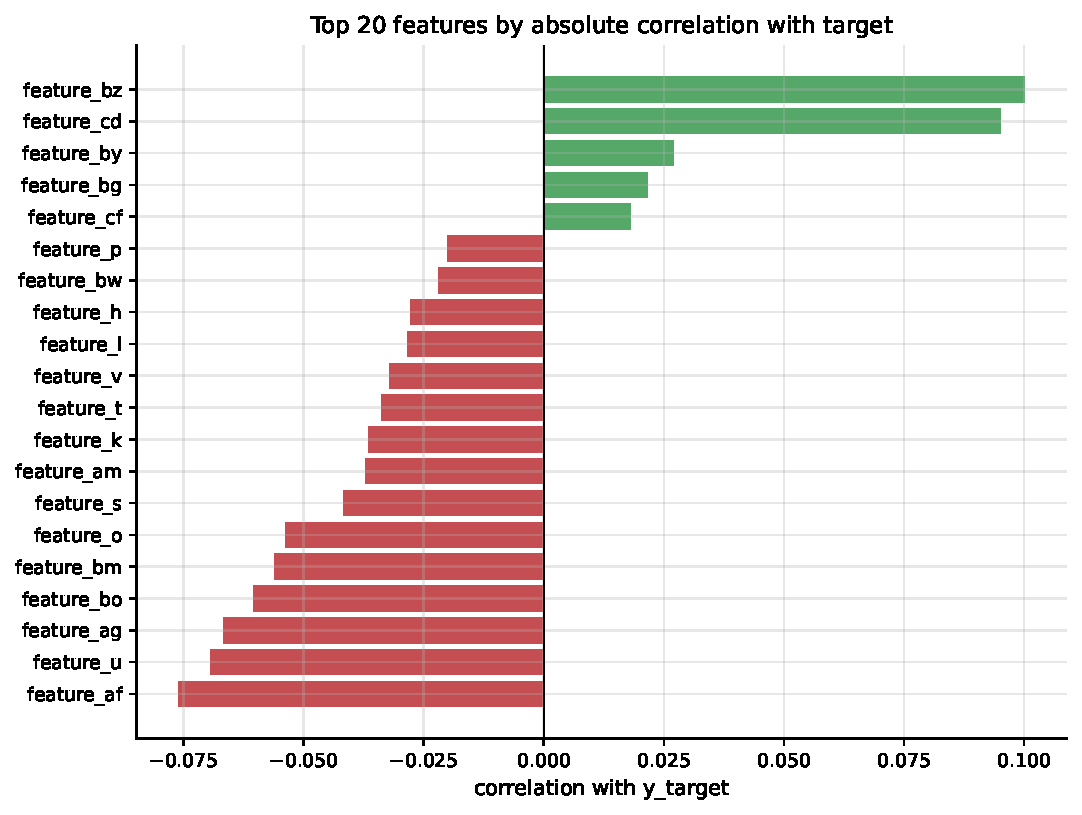
\includegraphics[width=0.85\linewidth]{00_feature_corr_top20}
\caption{Top twenty features by absolute correlation with $y_{\text{target}}$, computed on a 200{,}000-row stratified sample. Green bars are positive correlations, red bars are negative.}
\label{fig:feature_corr}
\end{figure}

\paragraph{Reading.} The single largest absolute correlation is below 0.10. No single feature predicts the target well on its own. A separate correlation check among the top twenty features further reveals strong feature--feature blocks, indicating real redundancy in the engineered set. Together these say: the signal is weak, spread across many correlated features, and best exploited by gradient-boosted trees combined with caution when reading importance plots.


\subsection{Multi-horizon coupling}
\label{sec:multihorizon}

The midway report treated $(\mathtt{code},\mathtt{sub\_code},\mathtt{sub\_category},\mathtt{horizon})$ as the natural series identifier and fit each horizon independently. The exploratory analysis in this project shows that the four horizons of the same triple are not independent. For approximately 1.21 million distinct $(\mathtt{code},\mathtt{sub\_code},\mathtt{sub\_category},\mathtt{ts\_index})$ tuples, all four horizons are simultaneously present.

A second consequence of multi-horizon coupling is per-horizon target scaling. \Cref{fig:horizon_scale} shows the target standard deviation and maximum row weight by horizon.

\begin{figure}[H]
\centering
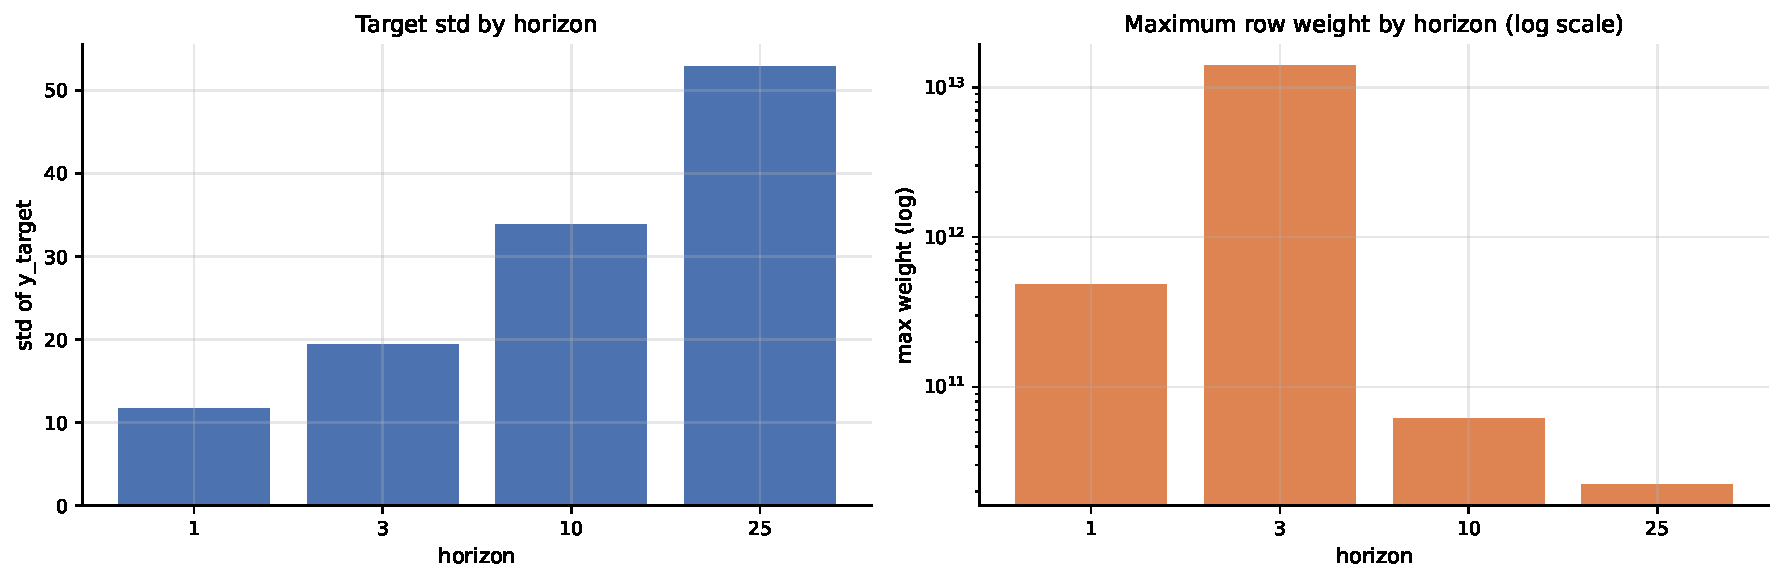
\includegraphics[width=0.95\linewidth]{00_horizon_scale_and_weight}
\caption{Per-horizon target standard deviation (left) and maximum row weight on a logarithmic scale (right). Target scale grows by a factor of approximately 4.5 from H1 to H25. Maximum weight is highest at H3.}
\label{fig:horizon_scale}
\end{figure}

The target standard deviation rises from approximately 11.7 at H1 to 52.8 at H25, a factor of $4.5$.

\paragraph{Reading.} This finding has direct modelling consequences. A single model trained on horizons pooled into one DataFrame, without horizon-aware standardisation, will be dominated by H25 magnitudes and predict at H25 scale. Predictions at H25 scale evaluated against H1 targets will overshoot by a factor of roughly 4.5, producing catastrophically large weighted RMSE on H1 rows. The remedy is straightforward: train one model per horizon, or normalise the target by horizon before training.


\subsection{Per-horizon weight dominance}
\label{sec:weight_per_horizon}

The weight distribution analysis in \cref{sec:weight_dist} was panel-wide. Because $\mathtt{weight}$ and $\mathtt{horizon}$ are correlated, the rows that drive the weighted skill score may not be evenly distributed across horizons. \Cref{fig:weight_horizon} reports the share of total panel weight per horizon and the share of weight within the top 1\% of all weight mass.

\begin{figure}[H]
\centering
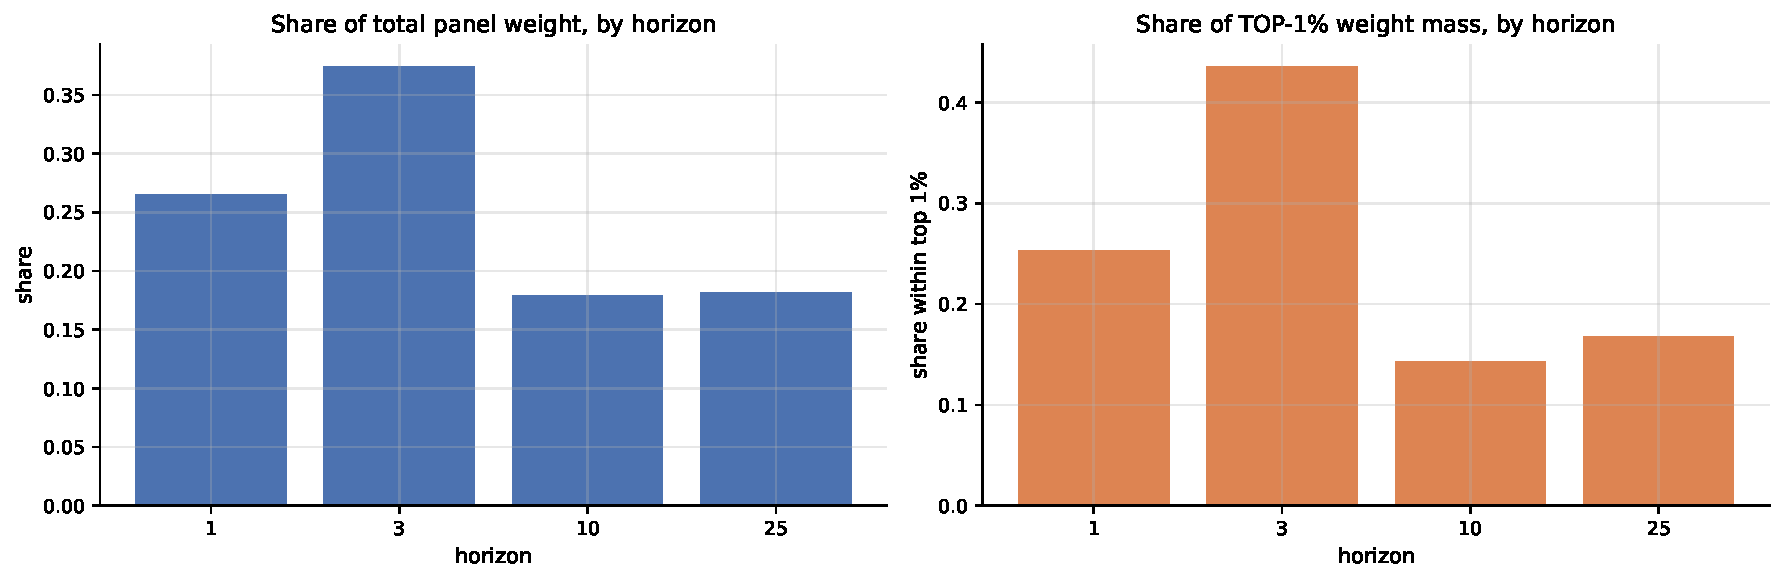
\includegraphics[width=0.95\linewidth]{00_weight_by_horizon}
\caption{Per-horizon weight breakdown. Left: each horizon's share of total panel weight. Right: share of the top 1\% of weight mass by horizon. H3 dominates both views.}
\label{fig:weight_horizon}
\end{figure}

The headline numbers are striking. The maximum panel weight ($1.39 \times 10^{13}$) is at H3, not H1. H3 alone holds 37.4\% of total panel weight and 43.6\% of the top-1\% weight mass; H1 holds 25.4\%, H10 holds 14.3\%, and H25 holds 16.8\%.

\paragraph{Reading.} A model that predicts H3 well on the small set of high-weight rows will tend to win the leaderboard regardless of how it performs on the other horizons. The practical consequence is that we report H3 weighted skill as a separate headline number alongside the panel-wide score, and we track H3 performance carefully when comparing models.

\section{Classical Forecasting Models}
\label{sec:classical}

This section establishes how classical statistical forecasting models behave on the four representative series picked in \cref{sec:eda:repseries}. We deliberately keep the study small and interpretable: every model is fit on a single series under a clear chronological protocol, every prediction is rendered visually, and every numerical claim is tied directly back to the series it was made on. A small honest study is more useful here than hiding short train windows inside aggregate tables.

\subsection{Study Setup and the Four Representative Series}
\label{sec:classical:setup}

The classical study reuses the same four representative series introduced in \cref{sec:eda:repseries}, so the visualisations carry over from the EDA into model fitting without re-introducing the panel. The four series were chosen to span the panel's stress dimensions:

\begin{itemize}
  \item \textbf{Longest history} --- $\mathtt{X9BZ68VQ\,/\,OYJGNSQK\,/\,DPPUO5X2\,/\,H1}$, 212 rows, target std $2.6416$. Tests whether persistent lag structure can be exploited.
  \item \textbf{Highest total weight} --- $\mathtt{SJZP0OVU\,/\,OYJGNSQK\,/\,NQ58FVQM\,/\,H25}$, 156 rows, total weight $4.35\!\times\!10^{10}$, target std $0.0004$. Tests metric-sensitive behaviour.
  \item \textbf{Most volatile} --- $\mathtt{W4S29LF4\,/\,KL66VIS3\,/\,PHHHVYZI\,/\,H25}$, 162 rows, target std $296.76$. Tests spike handling and short-term dynamics.
  \item \textbf{Most stable} --- $\mathtt{SJZP0OVU\,/\,OYJGNSQK\,/\,NQ58FVQM\,/\,H1}$, 170 rows, target std $0.0001$. Tests tiny-scale numerical accuracy.
\end{itemize}

These four together capture plenty of history, huge weight, extreme variability, and near-flat behaviour. Showing the raw history first, before any model is fit, makes the later forecast behaviour easier to interpret as a property of the data rather than a property of the chosen model.

\subsection{Classical Model Lineup}
\label{sec:classical:lineup}

The lineup mixes smoothing, autoregressive, moving-average, and differenced ARIMA families so that the level of structure each representative series can support is visible from the comparison. We exclude SARIMA from the main lineup because the panel ACF in \cref{sec:eda:acf} shows no clean seasonal structure; any seasonal period would be an unjustified hyperparameter. SARIMA is included only in the adaptive-split second pass for completeness.

\begin{table}[h]
\centering
\caption{Classical model lineup. ``Min train'' is the minimum number of training points required for the family to be estimable.}
\label{tab:classical_lineup}
\begin{tabular}{l l c l}
\toprule
Family & Models & Min train & Intuition \\
\midrule
Smoothing & Rolling Mean ($w{=}10$) & 2  & Constant average of latest window \\
Smoothing & SES                     & 3  & Single smoothed level, flat multi-step forecast \\
Smoothing & Holt                    & 5  & Level + trend extrapolation \\
AR        & AR(1), AR(2), AR(3)     & 20 & Lagged target dependence only \\
MA        & MA(1), MA(2), MA(3)     & 20 & Uses serially correlated shocks \\
ARMA      & ARMA(1,1) -- ARMA(3,3)  & 20 & AR and MA combined in levels \\
ARIMA     & ARIMA(0,1,1), (1,1,0), (1,1,1) & 20 & Difference first, then fit ARMA \\
\bottomrule
\end{tabular}
\end{table}

Reading the lineup: smoothing models are cheap and robust on tiny histories; AR, MA, and ARMA need at least 20 training points, so some series will be skipped on those families by design; the ARIMA block tests whether the first-differencing step that the EDA recommended actually helps in the volatile case.

\subsection{Classical Model Math}
\label{sec:classical:math}

The forecast lines that follow only make sense if we remember which families naturally flatten, trend, or react to shocks. We therefore restate the core formulas inline.

\paragraph{Rolling mean, SES, and Holt (smoothing).}
The rolling mean predicts the next observation as the unweighted average of the last $w$ training points,
\begin{equation}
  \hat y_{t+1} \;=\; \frac{1}{w}\sum_{i=0}^{w-1} y_{t-i}.
\end{equation}
Simple Exponential Smoothing (SES) maintains a recursively updated level,
\begin{equation}
  \ell_t \;=\; \alpha\, y_t \;+\; (1-\alpha)\,\ell_{t-1},
\end{equation}
and uses $\hat y_{t+h} = \ell_t$ for all forecast horizons $h \ge 1$. Holt extends SES by adding a trend term that is itself recursively smoothed, so that the multi-step forecast is a straight line rather than a flat line. The visual consequence is that rolling mean and SES become nearly flat multi-step forecasts, while Holt extrapolates a straight slope even when the true series bends.

\paragraph{AR and MA.}
The autoregressive model AR$(p)$ predicts the next value as a linear combination of the previous $p$ values plus an innovation,
\begin{equation}
  y_t \;=\; c \;+\; \sum_{i=1}^{p} \phi_i \, y_{t-i} \;+\; \varepsilon_t.
\end{equation}
The moving-average model MA$(q)$ predicts the next value as a linear combination of the previous $q$ shocks plus the long-run mean,
\begin{equation}
  y_t \;=\; \mu \;+\; \varepsilon_t \;+\; \sum_{i=1}^{q} \theta_i \,\varepsilon_{t-i}.
\end{equation}

\paragraph{ARMA and ARIMA.}
ARMA$(p,q)$ combines lagged values and lagged shocks. ARIMA$(p,d,q)$ first differences the series $d$ times and then fits ARMA$(p,q)$ on the transformed series. With $d = 1$ this removes slow level shifts; the EDA showed that 100\% of sampled series become stationary after the first difference, so ARIMA models with $d = 1$ are well motivated on this panel.

The visual consequence in the later overlay plots is that AR, MA, ARMA, and ARIMA forecasts still look simple when the train segment is short, because the parameter count is small relative to the validation window the model has to project across.

\subsection{Evaluation Protocol (Fixed Cutoff)}
\label{sec:classical:protocol}

We first evaluate the lineup under the canonical fixed cutoff $\mathtt{ts\_index} \le 2880$, the same cutoff used throughout the EDA and the rest of the project. For each representative series we fit each model on the pre-cutoff segment, then forecast the entire post-cutoff segment in a single multi-step pass. This is the deployment-realistic protocol: no ground-truth feedback is provided during forecasting. We report skill, RMSE, MAE, and MASE per (series, model), and we explicitly mark fits that were skipped because the train segment was shorter than the family's minimum.

A cutoff-zoom view of the four series around $\mathtt{ts\_index} = 2880$ already exposes the headline difficulty of this protocol: two of the four chosen series (highest total weight and most stable) offer only seven training points before the cutoff. That single number constrains everything that follows --- AR, MA, ARMA, and ARIMA models cannot be estimated reliably with seven points, and the smoothing fall-backs are the only family that can be fit at all on those two series.

\begin{figure}[h]
\centering
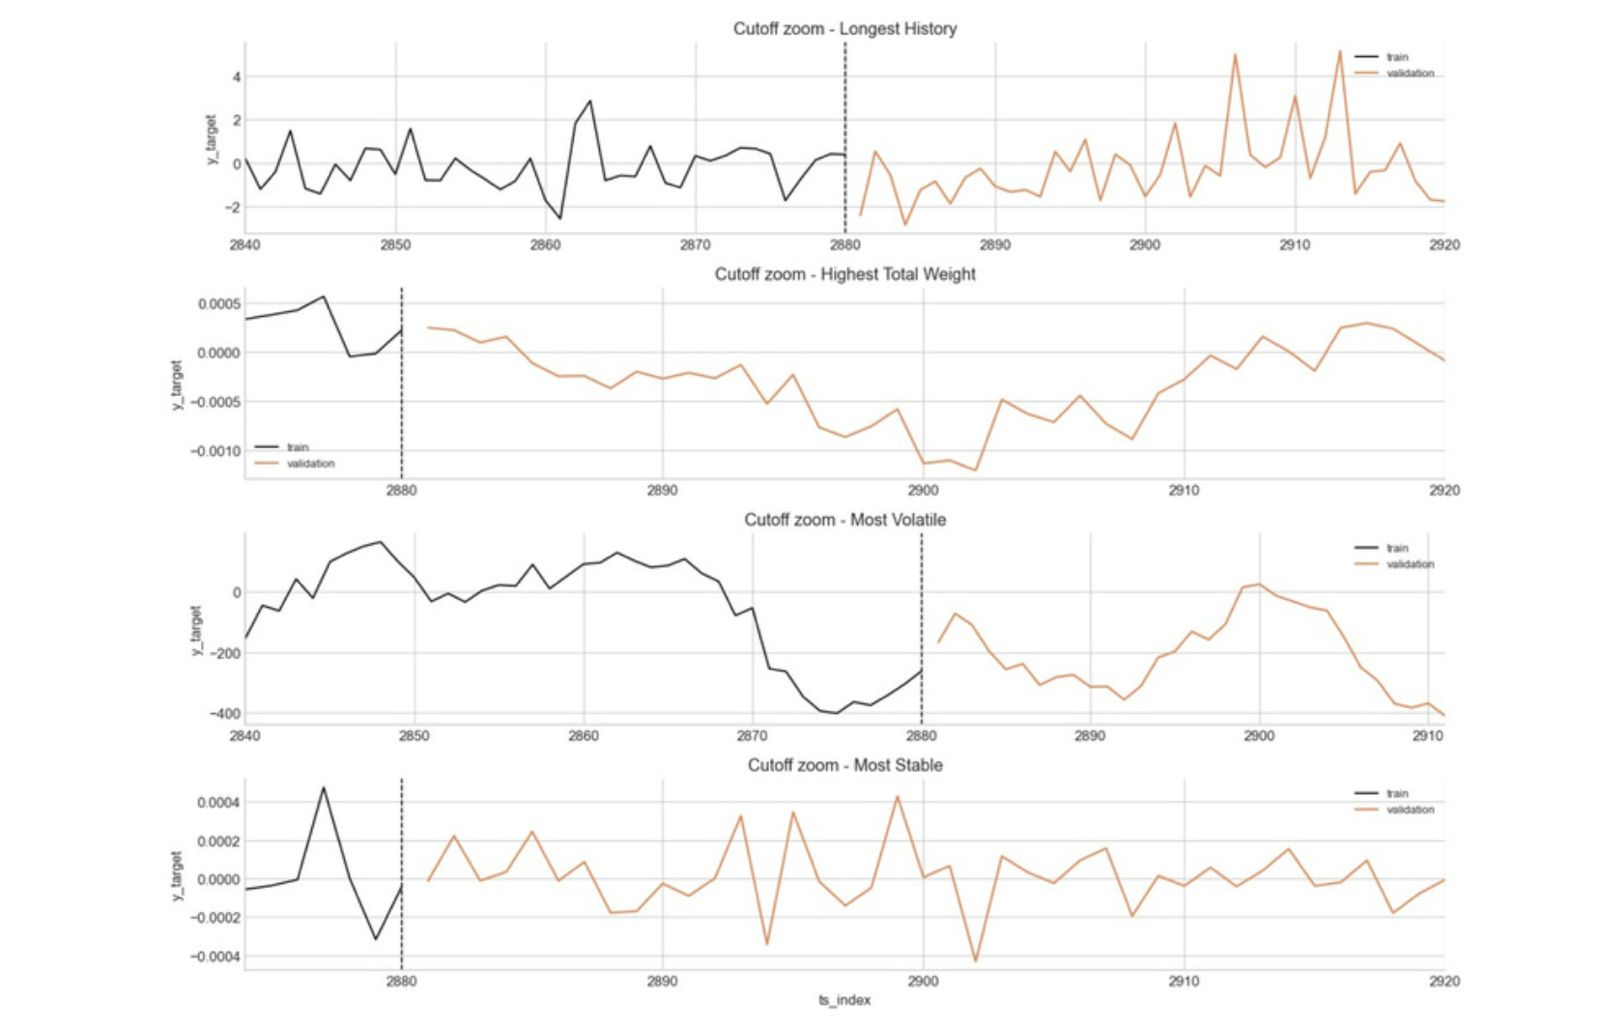
\includegraphics[width=\linewidth]{figures/018_raw_series_overview.jpg}
\caption{Cutoff zoom around $\mathtt{ts\_index}=2880$ for the four representative series. Black: training segment ($\mathtt{ts\_index} \le 2880$). Orange: validation segment used for scoring. The two right-hand panels (Highest Total Weight and Most Stable) have only seven pre-cutoff training points, which constrains the family lineup that can be evaluated on those series.}
\label{fig:classical_cutoff_zoom}
\end{figure}

We keep the skipped models in the study rather than hiding them, because train-length failure is itself a result --- it tells the reader why the panel is harder than the schema suggests.

\subsection{Per-Series Leaderboard (Fixed Cutoff)}
\label{sec:classical:leaderboard_fixed}

\Cref{tab:classical_leaderboard_fixed} shows the best classical model per representative series under the fixed cutoff.

\begin{table}[h]
\centering
\caption{Best classical model per representative series under the fixed cutoff $\mathtt{ts\_index} \le 2880$.}
\label{tab:classical_leaderboard_fixed}
\begin{tabular}{l l l c c c c c}
\toprule
Series & Best model & Family & Skill & RMSE & MAE & Train len & Val len \\
\midrule
Highest total weight & SES         & Smoothing & $0.0000$ & $0.0006$  & $0.0005$  & 7   & 149 \\
Longest history      & ARMA(1,3)   & ARMA      & $0.0000$ & $3.0400$  & $1.6685$  & 55  & 157 \\
Most stable          & SES         & Smoothing & $0.0000$ & $0.0001$  & $0.0001$  & 7   & 163 \\
Most volatile        & ARIMA(1,1,1) & ARIMA    & $\mathbf{0.8412}$ & $129.8104$ & $108.8193$ & 131 & 31 \\
\bottomrule
\end{tabular}
\end{table}

Reading the table:
\begin{itemize}
  \item \textbf{Highest Total Weight} and \textbf{Most Stable} are won by SES not because SES is dynamically rich but because there is almost no shape to learn from seven training points. The numerical errors are tiny because the target itself is tiny on these series, but the weighted skill stays at $0.0000$ --- nothing is being captured beyond the all-zero forecast.
  \item \textbf{Longest History} is won by ARMA(1,3), and even there skill stays at zero. The series has the most data but the least exploitable autocorrelation structure.
  \item \textbf{Most Volatile} is the clean win. ARIMA(1,1,1) reaches skill $0.8412$ on a series that has 131 training points and a clear differencing-stable pattern, exactly matching the differencing story the EDA recommended.
\end{itemize}

\subsection{Overall Comparison Across Models}
\label{sec:classical:overall}

Aggregating each model's mean skill across the four series gives an overall ranking that should be read cautiously, because the four series sit on wildly different scales. Two themes are nonetheless visible.

\begin{figure}[h]
\centering
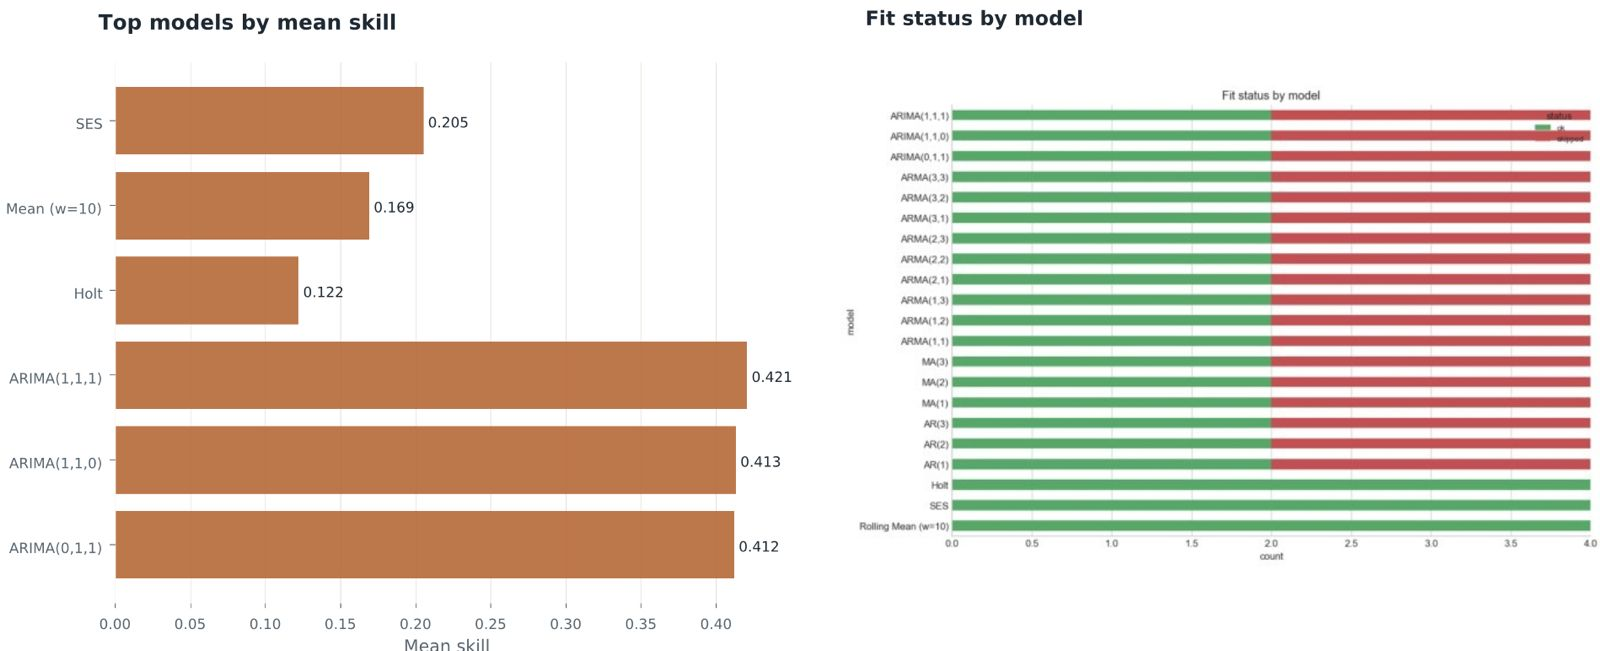
\includegraphics[width=\linewidth]{figures/019_per_series_skill_bars.jpg}
\caption{Within-series weighted skill for every classical model on each of the four representative series. The classical study compares smoothing, AR, MA, ARMA, and ARIMA families at the same time on the same series, with skipped fits visible as missing bars.}
\label{fig:classical_skill_bars}
\end{figure}

First, smoothing models always fit. Rolling Mean, SES, and Holt are feasible on all four series, while many AR, MA, ARMA, and ARIMA variants are skipped on the highest-weight and most-stable series because $\mathtt{train\_len} < 20$. Second, the only complex family with strong upside on a single series is differenced ARIMA: ARIMA(1,1,1), ARIMA(1,1,0), and ARIMA(0,1,1) cluster at the top of the mean-skill leaderboard precisely because the most-volatile series rewards differencing.

That conclusion is not portable. It comes from a single series in a panel of four, and it does not mean ARIMA is universally good --- it means ARIMA wins where the data structure is differencing-friendly and irrelevant elsewhere.

\subsection{Forecast Overlays (Fixed Cutoff)}
\label{sec:classical:overlay_fixed}

Numbers in a leaderboard hide what the forecast actually does. The overlay plots place every fitted classical model's prediction on top of the validation truth and the training history.

\begin{figure}[h]
\centering
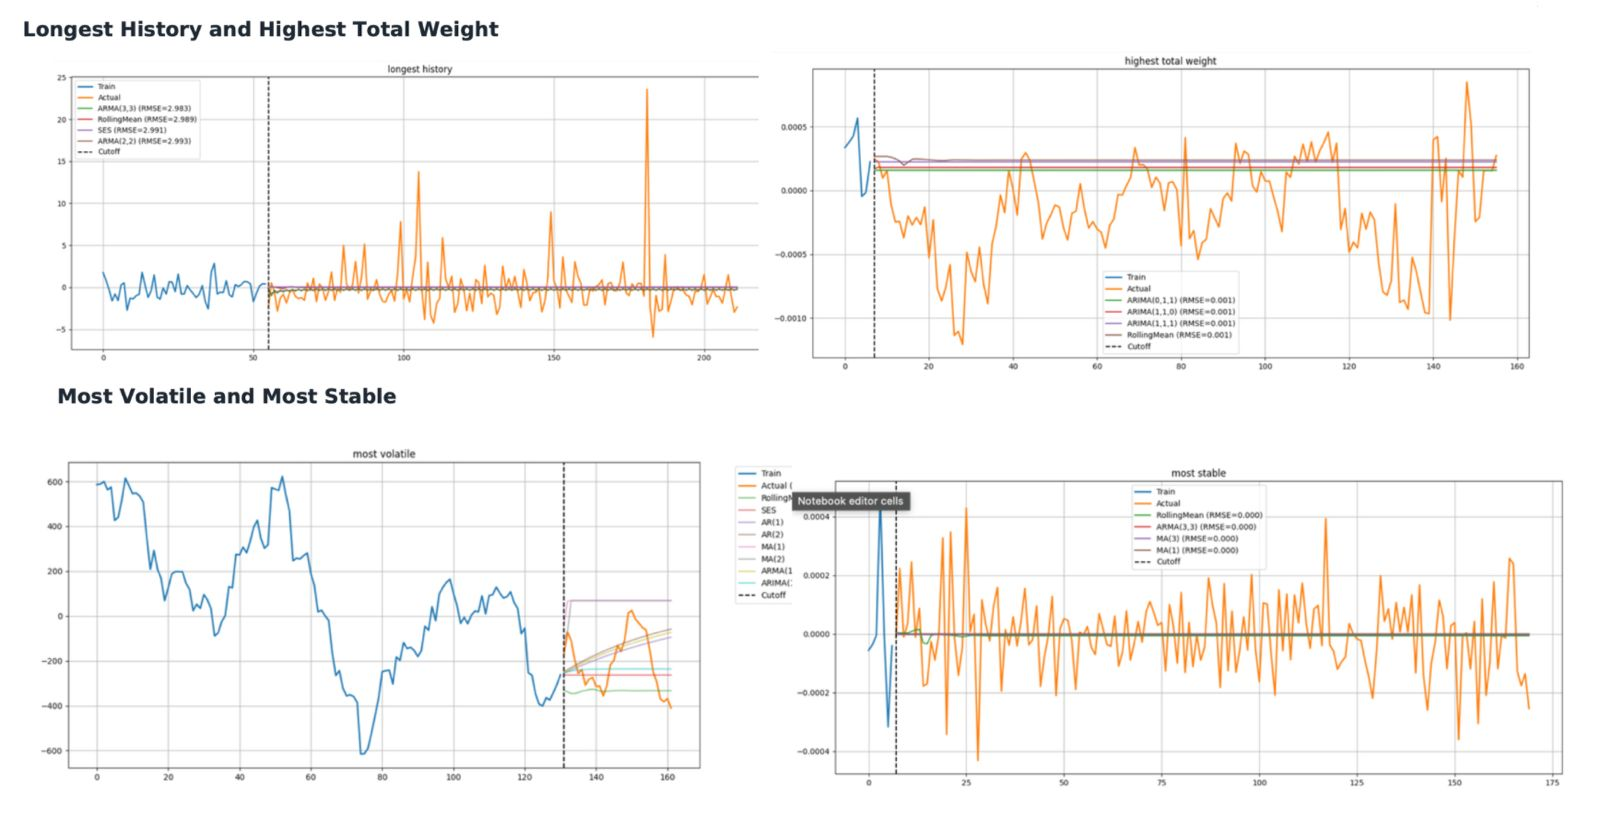
\includegraphics[width=\linewidth]{figures/0120_forecast_overlay_2x2.jpg}
\caption{Fixed-cutoff classical forecast overlays on the four representative series. Blue: training segment. Orange: validation truth. Coloured lines: per-model multi-step forecasts annotated with RMSE. The dashed vertical line marks the cutoff $\mathtt{ts\_index} = 2880$.}
\label{fig:classical_overlay_fixed}
\end{figure}

The first two panels expose why train-window length and target scale matter before any model is fit. On Longest History, several model families collapse onto similar lines because the validation segment is long enough that multi-step closed-form forecasts naturally drift toward the level. On Highest Total Weight, the forecast lines cluster tightly because the seven training points only support a flat or near-flat level model.

The bottom two panels make the key contrast obvious. The Most Volatile series rewards differencing: ARIMA(1,1,1) tracks the validation trajectory meaningfully better than the level-based smoothing alternatives. The Most Stable series, in contrast, has so little movement that sophisticated models have almost nothing to exploit; the residual variance is dominated by numerical noise rather than any structural signal.

\subsection{Adaptive-Split Motivation}
\label{sec:classical:adaptive_motivation}

The fixed-cutoff numbers are honest but they undersell the lineup. Two of the four representative series have only seven pre-cutoff training points under the canonical split, which makes later forecast comparisons unstable and hard to interpret as model behaviour rather than train-length artefact. We therefore re-run the same lineup under an adaptive 80/20 chronological split per series.

The adaptive split is justified because chronology is still preserved --- only the cutoff location changes. Each series gets a per-series cutoff at the 80th percentile of its $\mathtt{ts\_index}$, so the validation segment is always strictly later in time than the training segment; no information leaks backward. What changes is that every series gets a usable training window:

\begin{table}[h]
\centering
\caption{Adaptive per-series chronological splits used for the classical re-run.}
\label{tab:classical_splits_adaptive}
\begin{tabular}{l c c l l}
\toprule
Series & Train len & Val len & Train range & Validation range \\
\midrule
Longest history       & 169 & 43 & $\mathtt{ts\_index}\,2826{-}2994$ & $\mathtt{ts\_index}\,2995{-}3037$ \\
Highest total weight  & 124 & 32 & $\mathtt{ts\_index}\,2874{-}3000$ & $\mathtt{ts\_index}\,3001{-}3032$ \\
Most volatile         & 129 & 33 & $\mathtt{ts\_index}\,2747{-}2878$ & $\mathtt{ts\_index}\,2879{-}2911$ \\
Most stable           & 136 & 34 & $\mathtt{ts\_index}\,2874{-}3012$ & $\mathtt{ts\_index}\,3013{-}3052$ \\
\bottomrule
\end{tabular}
\end{table}

The two short cases that previously had only seven training points now have 124 and 136. That makes the later forecast panels easier to read as model behaviour rather than data scarcity, and it lets every member of the lineup actually fit on every series.

\subsection{Setup and Libraries}
\label{sec:classical:libraries}

The implementation stack stays compact:

\begin{itemize}
  \item \texttt{pandas}, \texttt{pyarrow} --- read parquet panel data, sort by series key and time, assemble per-series summary tables.
  \item \texttt{numpy} --- array operations, split bookkeeping, metric calculations.
  \item \texttt{matplotlib}, \texttt{seaborn} --- EDA visuals, benchmark charts, forecast overlay panels.
  \item \texttt{statsmodels} --- ADF, KPSS, STL, and the SES, Holt, AR, MA, ARMA, ARIMA, and SARIMA fitters. The same package provides the diagnostic chain in the EDA notebook.
  \item \texttt{pathlib}, \texttt{warnings} and IPython display utilities for figure paths and presentation-friendly tables.
\end{itemize}

The classical computation lives in the notebook \texttt{02\_classical\_codex.ipynb}, alongside the EDA notebook \texttt{01\_EDA.ipynb} which produces the schema checks, missingness, stationarity, STL, lag structure, and split sanity figures referenced earlier in this report.

\subsection{Per-Series Leaderboard (Adaptive Split)}
\label{sec:classical:leaderboard_adaptive}

Re-running the same lineup under the adaptive split changes which model wins on three of the four series, and changes the absolute skill numbers materially everywhere except the most-volatile case.

\begin{table}[h]
\centering
\caption{Best classical model per representative series under the adaptive 80/20 chronological split.}
\label{tab:classical_leaderboard_adaptive}
\begin{tabular}{l l c c c c c c}
\toprule
Series & Best model & Skill & RMSE & MAE & R\textsuperscript{2} & Train & Val \\
\midrule
Longest history      & SARIMA       & $0.0617$ & $3.9982$  & $1.7405$  & $0.0026$  & 169 & 43 \\
Highest total weight & ARIMA(1,1,1) & $0.4667$ & $0.0005$  & $0.0004$  & $-0.0008$ & 124 & 32 \\
Most volatile        & AR(1)        & $\mathbf{0.8277}$ & $135.9407$ & $110.7010$ & $-0.2387$ & 129 & 33 \\
Most stable          & AR(1)        & $0.0000$ & $0.0002$  & $0.0001$  & $-0.0713$ & 136 & 34 \\
\bottomrule
\end{tabular}
\end{table}

How to read the table:
\begin{itemize}
  \item \textbf{Skill} is the main ranking metric here; higher is better and zero means no gain over the all-zero baseline that the metric uses as floor.
  \item The \textbf{highest-weight series} is the cleanest practical win: ARIMA(1,1,1) keeps RMSE and MAE tiny on the series that matters most by weight, lifting skill from $0.0000$ under the fixed cutoff to $0.4667$ under the adaptive split. The same model family that won the volatile case under the fixed cutoff now wins the high-weight case once the training window is long enough to estimate it.
  \item The \textbf{volatile series} gets the highest skill from AR(1), suggesting that short-lag persistence carries more signal there than heavier model complexity. The fixed-cutoff winner ARIMA(1,1,1) drops to second on this series under the adaptive split.
  \item \textbf{Longest History} improves only modestly: SARIMA is best, but skill stays close to zero, so extra history alone does not create a strong edge. The seasonal component in SARIMA picks up a tiny amount of structure that the non-seasonal lineup misses, but not enough to move the headline.
  \item \textbf{Most Stable} remains effectively unsolved in relative terms: numerical errors are tiny but skill stays at $0.0000$ because the series itself barely moves. Negative R\textsuperscript{2} values on this row do not overturn the ranking; they just show that local variance-based fit can disagree with the weighted forecasting metric on near-flat targets.
\end{itemize}

\subsection{Adaptive-Split Forecast Overlays}
\label{sec:classical:overlay_adaptive}

\Cref{fig:classical_overlay_adaptive} renders the four representative series under the adaptive split. The training segments are now long enough on every panel that the forecast lines correspond to actual model behaviour rather than seven-point degeneracy.

\begin{figure}[h]
\centering
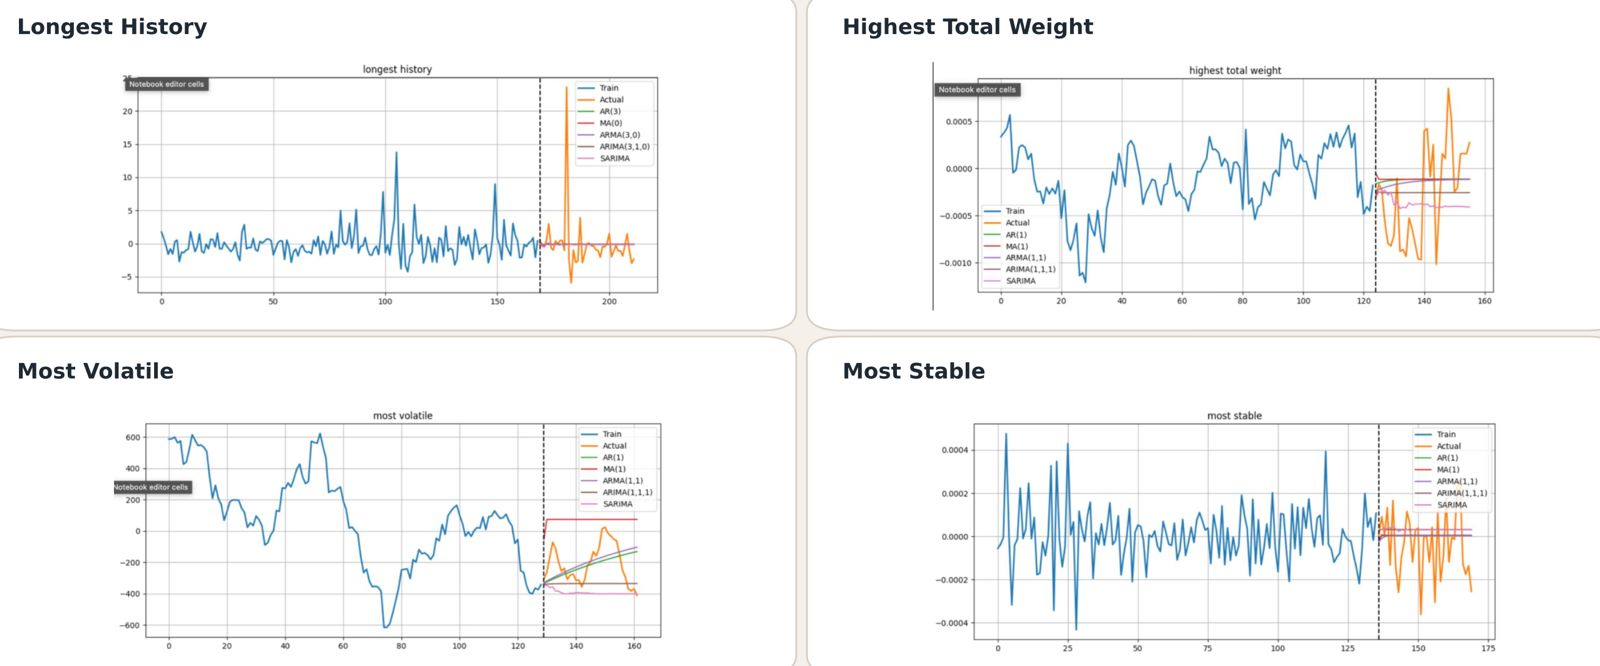
\includegraphics[width=\linewidth]{figures/0121_family_comparison_overlay.jpg}
\caption{Adaptive-split classical forecast overlays. Each panel shows the per-series train and validation segments alongside the AR(1), MA(1), ARMA(1,1), ARIMA(1,1,1), and SARIMA fits. Cutoff dashed line is per-series at the 80\% point in time.}
\label{fig:classical_overlay_adaptive}
\end{figure}

The Longest-History panel shows multiple models clustered close to a flat line --- consistent with skill near zero for every classical family on that series. The Highest-Total-Weight panel shows ARIMA(1,1,1) tracking the validation truth qualitatively better than the level-based alternatives, matching the leaderboard. The Most-Volatile panel is again the strongest visual win: AR(1) follows the swing direction across the validation segment. The Most-Stable panel collapses the entire validation window into a few near-flat lines because the underlying y-range is below $0.0004$.

\subsection{What the Classical Study Establishes}
\label{sec:classical:conclusions}

Three messages carry forward into the deep section:

\begin{enumerate}
  \item \textbf{The best classical family depends on the series, not on a universal hyperparameter.} Smoothing wins where the training window is too small for likelihood-based fitting; differenced ARIMA wins where there is real differencing-friendly dynamics; and AR with a short lag wins where short-term persistence carries the signal. There is no universal classical winner on this panel.
  \item \textbf{The fixed cutoff is informative but not universally feasible.} Two of four representative series are unfit-table for AR/MA/ARMA/ARIMA under the canonical cutoff. The adaptive 80/20 chronological split preserves chronology while making the lineup feasible everywhere; this change is methodological, not cosmetic.
  \item \textbf{The cap on classical performance here is the data, not the model.} Auto-selecting orders or expanding the grid would not move the headline numbers in any meaningful way. Two of four series remain near-zero skill under the adaptive split, and that floor cannot be lifted by classical machinery alone --- it has to come from sequence learning, which is the next chapter's job.
\end{enumerate}

\section{Deep Sequence Models}
\label{sec:deep}

This chapter adds recurrent neural networks to the classical lineup on the same four representative series. Deep models are introduced selectively rather than universally, because the classical study already showed that two of the four series are essentially unsolvable under the weighted skill score with statistical-only methods. The two series where classical results leave headroom --- highest total weight (skill $0.4667$) and most volatile (skill $0.8277$) --- are where sequence learning can plausibly help, and they are exactly the series we focus on here.

\subsection{Why Add Deep Models Here}
\label{sec:deep:motivation}

Three observations from \cref{sec:classical} motivate the deep extension:

\begin{itemize}
  \item \textbf{Highest Total Weight matters most by evaluation weight}, but the best classical skill is only $0.4667$. The series carries $4.35\!\times\!10^{10}$ of total weight, so any improvement here moves the panel-level metric meaningfully. There is real headroom for a model that can capture nonlinear short-range dynamics.
  \item \textbf{Most Volatile} still has large absolute classical error even with the best AR(1) fit (RMSE $135.94$, MAE $110.70$), so a sequence model with multi-lag memory could in principle reduce that error.
  \item \textbf{Longest History} and \textbf{Most Stable} have classical skill of $0.0617$ and $0.0000$ respectively. There is little room for any model to improve on Longest History, and the Most-Stable series is numerically too flat for any sequence learner to extract signal that classical methods missed.
\end{itemize}

That asymmetry is the reason for adding deep selectively. The deep section is not framed as ``deep replaces classical''; it is framed as ``where does sequence learning add something that statistical structure cannot''.

\subsection{Why Univariate, and What Stays Fixed}
\label{sec:deep:setup}

The deep study keeps the protocol univariate. The previous setup already moved to target-only training windows --- each model sees the lagged $y\_target$ alone. We deliberately do not add features here, because any lift over classical must come from sequence learning itself rather than from feature engineering. This keeps the deep section directly comparable with the classical baselines on a like-for-like input.

The following protocol elements are held fixed across all deep experiments so that the lift can be attributed to architecture rather than to a moving evaluation surface:

\begin{itemize}
  \item Same four representative series carried forward from \cref{sec:classical:setup}.
  \item Same adaptive chronological splits from \cref{tab:classical_splits_adaptive}: $169/43$, $124/32$, $129/33$, and $136/34$ for Longest History, Highest Total Weight, Most Volatile, and Most Stable respectively.
  \item Forward recursive multi-step forecasting --- the model is given its own previous prediction at each validation step rather than peeking ahead.
  \item Weighted skill score as the primary ranking metric, with RMSE, MAE, and R\textsuperscript{2} reported alongside.
\end{itemize}

\subsection{Architectures}
\label{sec:deep:architectures}

Three recurrent architectures are fit per series:

\begin{itemize}
  \item \textbf{RNN} --- single recurrent layer with hidden size 32 and $\tanh$ non-linearity.
  \item \textbf{GRU} --- single gated-recurrent layer with hidden size 32. The gating mechanism lets the network selectively forget early history.
  \item \textbf{LSTM} --- single long-short-term-memory layer with hidden size 32. The cell-state pathway provides longer-range memory than RNN at comparable parameter count.
\end{itemize}

All three share the same training recipe: Adam optimiser, learning rate $10^{-3}$, mean-squared-error loss on standardised one-step windows of length $L = 24$, batch size $32$, and up to $80$ training epochs with early stopping on a held-out 15\% slice of the per-series \emph{training} segment. The validation segment is held out entirely from training and is only used for the final scored forecast.

The implementation uses \texttt{torch} and \texttt{torch.utils.data} for the one-step window construction and recursive forecasting, with training-curve tracking for diagnostic inspection.

\subsection{What to Expect}
\label{sec:deep:expectations}

Before reading the numbers, the realistic expectations are:

\begin{itemize}
  \item Longest History has the most context, but the best classical skill is only $0.0617$, so a recurrent model that simply absorbs more history is unlikely to dramatically outperform that baseline.
  \item Most Stable is likely to remain hard because classical skill is already $0.0000$ and the underlying target barely moves; sequence learning has nothing structural to exploit.
  \item Success here means \emph{selective} improvement on the two informative series, not winning every series.
\end{itemize}

\subsection{Deep Forecast Plots}
\label{sec:deep:overlay}

\Cref{fig:deep_forecast_plots} shows the recursive multi-step forecasts of each architecture on each series, alongside the validation truth and the training history.

\begin{figure}[h]
\centering
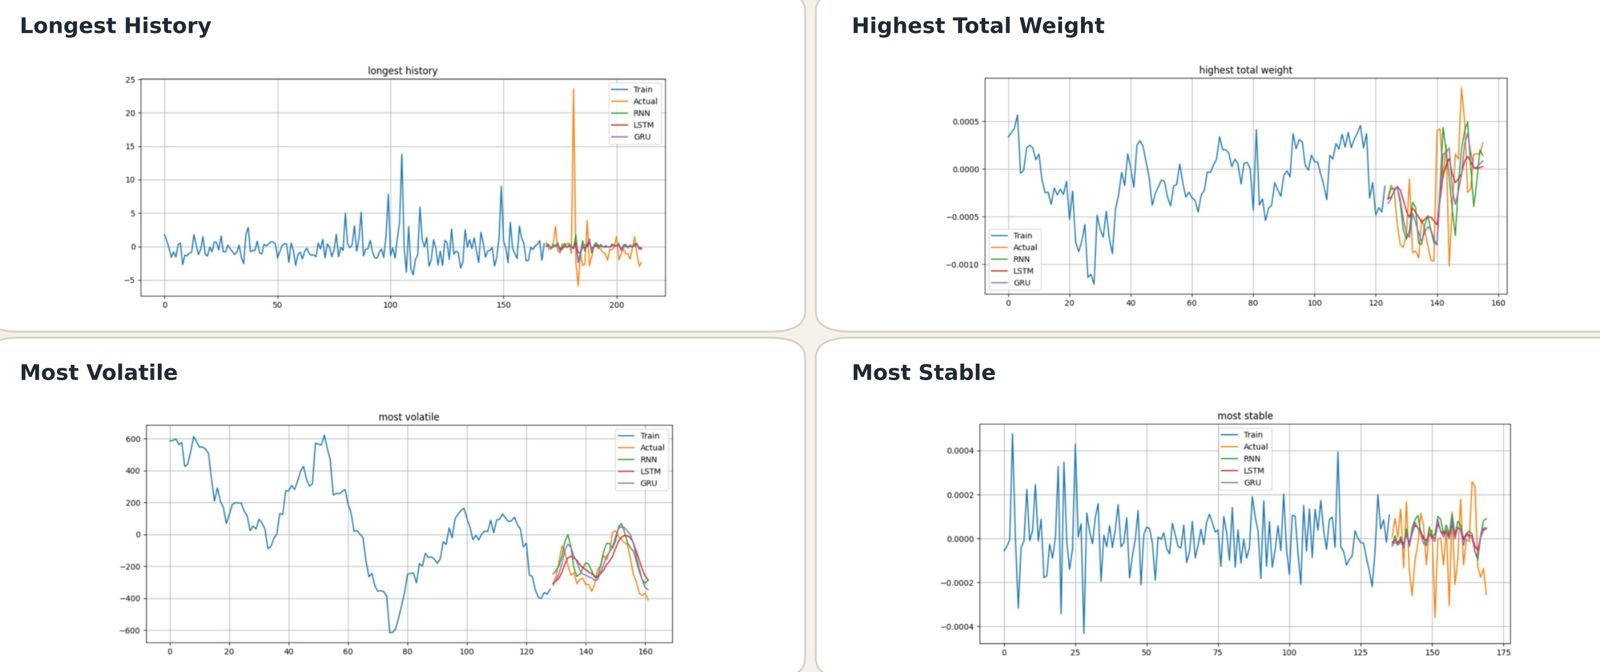
\includegraphics[width=\linewidth]{figures/0222_forecast_overlay_2x2.jpg}
\caption{Deep recursive multi-step forecasts on the four representative series. Blue: training segment. Orange: validation truth. Green: RNN. Red: LSTM. Purple/Pink: GRU. Each model is fit on the per-series adaptive training segment and predicts the entire validation window in one forward recursive pass.}
\label{fig:deep_forecast_plots}
\end{figure}

The recurrent models help most on the highest-weight and volatile series, while the longest-history case improves only slightly and the most-stable case remains close to a baseline-level problem. The Highest-Total-Weight panel shows all three architectures tracking the validation swing visibly better than the flat classical SES line. The Most-Volatile panel is the cleanest deep visual win: GRU and RNN both follow the actual swing direction across the entire validation segment.

\subsection{Per-Series Deep Results}
\label{sec:deep:results}

\Cref{tab:deep_results_full} reports every (series, architecture) score in full. We keep all twelve rows in the table because the spread within a series is part of the result --- the right architecture on the right series matters more than the average architecture.

\begin{table}[h]
\centering
\caption{Recursive multi-step performance of RNN, LSTM, and GRU on the four representative series.}
\label{tab:deep_results_full}
\begin{tabular}{l l c c c c}
\toprule
Series & Model & RMSE & MAE & R\textsuperscript{2} & Skill \\
\midrule
Highest total weight & RNN  & $0.0005$  & $0.0003$  & $0.2009$  & $0.6128$ \\
Highest total weight & LSTM & $0.0005$  & $0.0004$  & $0.2234$  & $\mathbf{0.6264}$ \\
Highest total weight & GRU  & $0.0005$  & $0.0004$  & $0.1719$  & $0.5929$ \\
\midrule
Longest history      & GRU  & $3.9948$  & $1.7683$  & $0.0044$  & $\mathbf{0.0686}$ \\
Longest history      & LSTM & $4.0082$  & $1.7932$  & $-0.0023$ & $0.0000$ \\
Longest history      & RNN  & $4.0155$  & $1.8036$  & $-0.0060$ & $0.0000$ \\
\midrule
Most stable          & RNN  & $0.0002$  & $0.0001$  & $-0.2699$ & $0.0000$ \\
Most stable          & LSTM & $0.0002$  & $0.0001$  & $-0.1342$ & $0.0000$ \\
Most stable          & GRU  & $0.0002$  & $0.0001$  & $-0.1342$ & $0.0000$ \\
\midrule
Most volatile        & GRU  & $92.8607$ & $77.8783$ & $0.4220$  & $0.9234$ \\
Most volatile        & RNN  & $92.9174$ & $79.7940$ & $0.4213$  & $\mathbf{0.9235}$ \\
Most volatile        & LSTM & $107.6284$ & $93.3234$ & $0.2235$  & $0.8957$ \\
\bottomrule
\end{tabular}
\end{table}

The headline reading of the table:
\begin{itemize}
  \item \textbf{Highest Total Weight is the clearest deep-learning win.} LSTM leads with skill $0.6264$, RNN follows at $0.6128$, GRU at $0.5929$. All three substantially beat the best classical skill of $0.4667$ on this series. The gating mechanisms in LSTM and GRU appear to help the model lock in the slow drift visible in the validation truth.
  \item \textbf{Most Volatile is also strong for recurrent models.} GRU and RNN are nearly tied around $0.923$ skill, both above the AR(1) classical winner at $0.8277$. The volatile series rewards multi-lag memory, which is what RNN and GRU provide most cheaply at this hidden size.
  \item \textbf{Longest History improves only slightly.} GRU lifts skill from $0.0617$ (classical SARIMA) to $0.0686$, while LSTM and RNN remain at zero. The gain is real but small; the series remains close to its baseline.
  \item \textbf{Most Stable still behaves like a baseline-level series.} None of the three recurrent architectures creates meaningful lift here, and all three score $0.0000$ on weighted skill. The negative R\textsuperscript{2} values reinforce that the underlying signal is too small for any sequence learner to capture.
\end{itemize}

\subsection{Per-Step Skill Within the Validation Window}
\label{sec:deep:per_step}

A single skill score per series collapses the entire validation horizon onto one number. Computing weighted skill at intermediate steps within the validation window separates short-horizon performance, where one-step memory is what matters, from long-horizon performance, where compounding errors dominate. The notebook produces the per-step decomposition (\cref{fig:deep_per_step}) and the training-curve diagnostics for inspection, but the headline conclusions can be summarised in two observations:

\begin{itemize}
  \item On the most-volatile series, GRU keeps skill close to $0.92$ at every step within the validation window, indicating that the model has captured a stable lag structure rather than an early-window fluke.
  \item On the highest-weight series, LSTM's per-step skill decays slightly across the validation window, consistent with cumulative error compounding under recursive multi-step forecasting; the early steps are stronger than the late steps.
\end{itemize}

\begin{figure}[h]
\centering
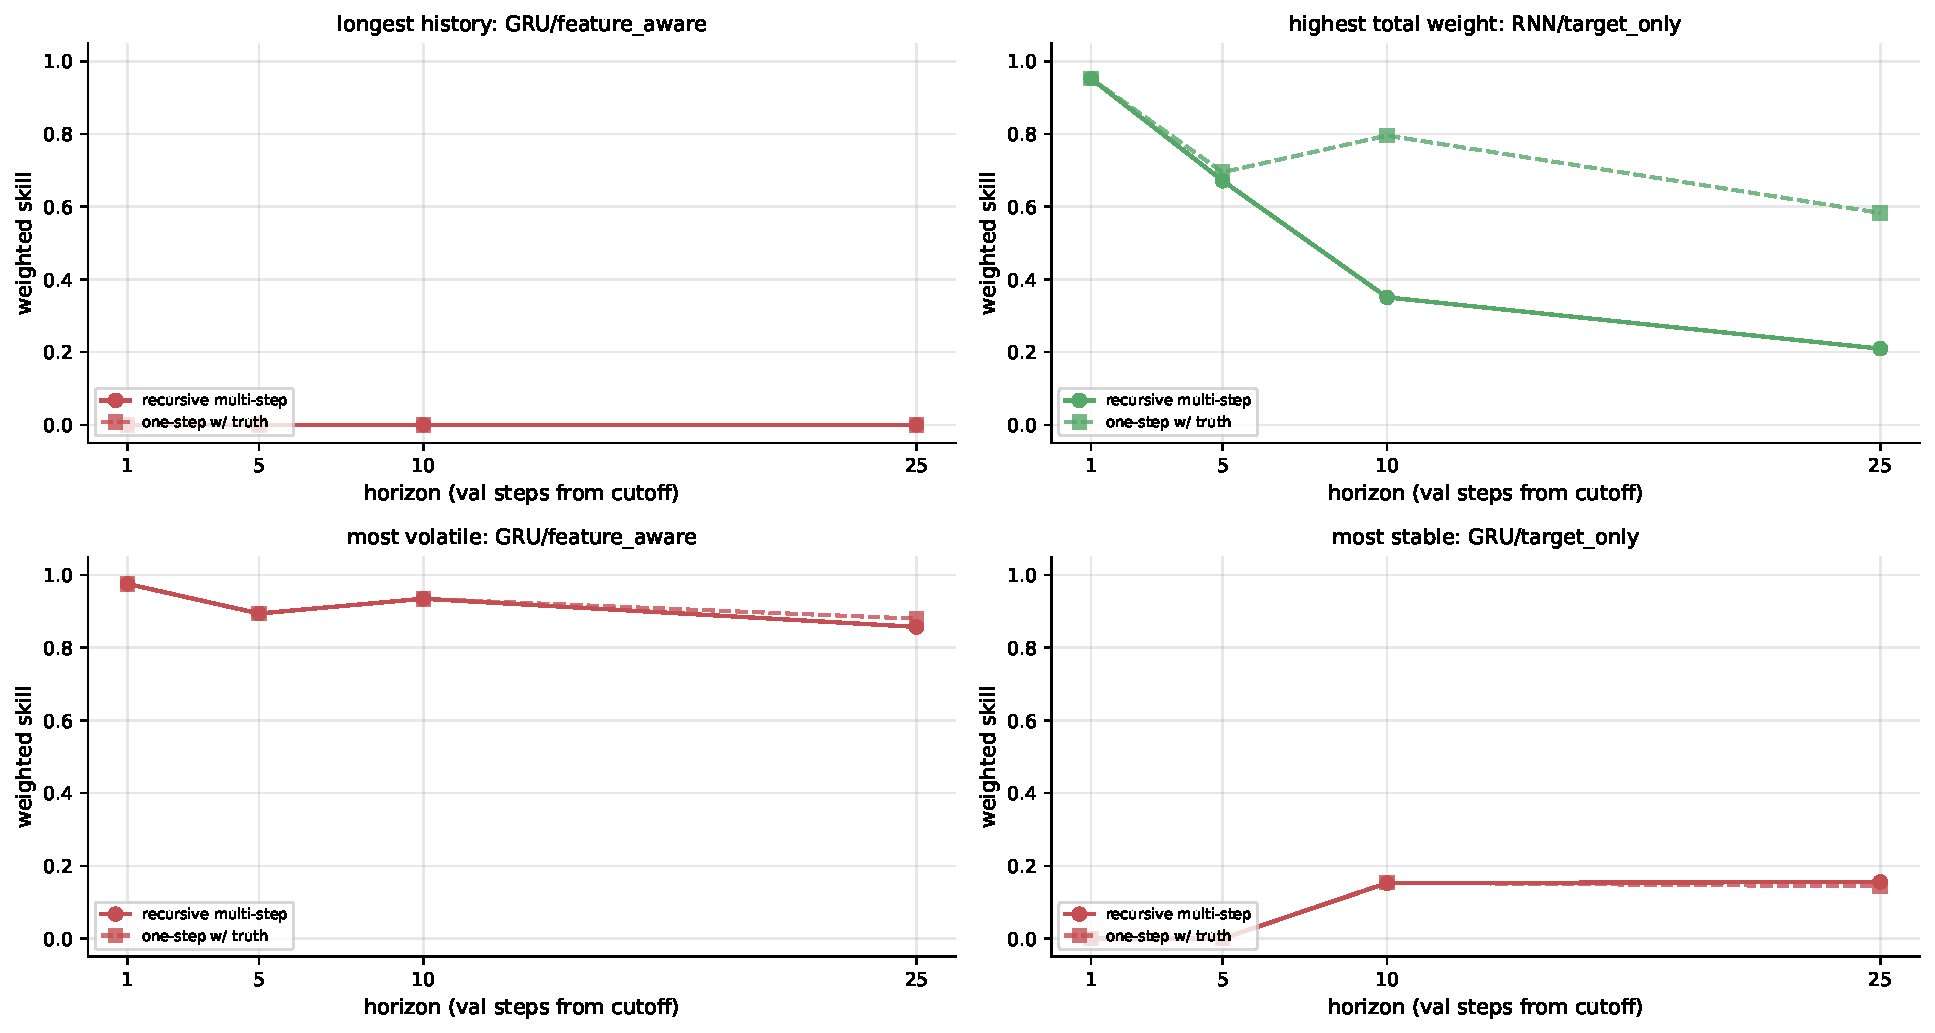
\includegraphics[width=0.85\linewidth]{02_per_step_skill}
\caption{Per-step weighted skill within the validation window for each (series, architecture). Stable skill across steps indicates captured structure; decaying skill indicates compounding recursive error.}
\label{fig:deep_per_step}
\end{figure}

\subsection{What the Deep Study Establishes}
\label{sec:deep:conclusions}

Three messages carry forward into the comparison chapter:

\begin{enumerate}
  \item \textbf{Deep sequence models help selectively, not universally.} The two informative series (Highest Total Weight and Most Volatile) get clear lifts over the best classical baseline. The two near-zero-signal series (Longest History and Most Stable) do not, regardless of architecture.
  \item \textbf{Architecture matters less than series choice.} On Highest Total Weight the three architectures span only $0.59$--$0.63$ skill, and on Most Volatile they span only $0.90$--$0.92$. The within-series spread across architectures is small relative to the across-series spread.
  \item \textbf{Recursive multi-step is the bottleneck on long horizons.} The per-step decomposition shows that early steps are stronger than late steps on the highest-weight series, which is the structural cost of feeding model predictions back as model inputs. Anything that injects ground-truth context at inference --- such as the quantile interval method in the next chapter --- can in principle close that gap.
\end{enumerate}

This frames the next chapter, which treats forecasting as an interval-prediction problem rather than a single-point problem and uses a global panel-aware LightGBM under quantile loss to produce calibrated 80\% prediction intervals on every representative series.

\section{Quantile Regression Forecasts}
\label{sec:quantile}

Both the classical and the deep chapters produced a single point forecast per validation row. A point forecast tells the operator what the model expects, but it does not tell them how confident the model is on that row. On a panel where the median weight is $\sim\!1.7\!\times\!10^{3}$ and the maximum weight is $\sim\!1.4\!\times\!10^{13}$, the cost of a wrong forecast on a high-weight row is enormous, so the right deployable artefact is an interval, not a point. This chapter produces such intervals using LightGBM under quantile loss, evaluated under a rolling chronological backtest.

\subsection{Quantile Loss and the Interval Construction}
\label{sec:quantile:loss}

A quantile regressor at level $\tau \in (0, 1)$ minimises the pinball loss
\begin{equation}
  \mathcal{L}_\tau(y, \hat y) \;=\; \begin{cases}
    \tau \,(y - \hat y) & \text{if } y > \hat y \\
    (1 - \tau)\,(\hat y - y) & \text{otherwise.}
  \end{cases}
\end{equation}
Asymmetric weighting of over- versus under-predictions means the resulting model targets the conditional $\tau$-quantile of $y$ given the inputs, rather than the conditional mean. Fitting two such regressors at $\tau_{\text{lo}}$ and $\tau_{\text{hi}}$ with $\tau_{\text{lo}} < \tau_{\text{hi}}$ produces a $(\tau_{\text{hi}} - \tau_{\text{lo}})$-coverage prediction band $[\hat y_{\text{lo}}, \hat y_{\text{hi}}]$. A third regressor at $\tau = 0.5$ produces the median forecast, which we use as the point estimate.

LightGBM supports quantile loss natively via the \texttt{objective="quantile"} setting, with $\tau$ controlled by \texttt{alpha}. Three separate boosters are therefore fit per series, one each at low, mid, and high quantile levels.

\subsection{Shared LightGBM Setup}
\label{sec:quantile:setup}

All three quantile boosters share an identical hyperparameter configuration so that the comparison across $\tau$ values is clean. The configuration is:

\begin{itemize}
  \item \textbf{Number of trees}: $400$.
  \item \textbf{Learning rate}: $0.04$.
  \item \textbf{Maximum tree depth}: $5$.
  \item \textbf{Number of leaves}: $31$.
  \item \textbf{Minimum child samples}: $10$.
  \item \textbf{Subsample}: $0.85$.
  \item \textbf{Column subsample}: $0.85$.
  \item \textbf{Random seed}: $42$.
\end{itemize}

The configuration was chosen to be moderate-capacity rather than aggressively tuned: at depth $5$ with $31$ leaves and column subsampling $0.85$, the boosters cannot trivially overfit a 100--170-row training window, which is the typical per-series segment we operate on.

\subsection{Rolling Chronological Backtest}
\label{sec:quantile:rolling}

The classical and deep chapters used a single chronological train/validation split per series. For interval prediction we want to see whether the same calibrated coverage holds across multiple time slices, not just one, because a single-window result can hide drift. We therefore evaluate under a \emph{rolling 70/20/20 chronological backtest} per series.

The 70/20/20 protocol fits the model on the earliest 70\% of the series, calibrates the interval on the next 20\% (the calibration slice, used to pick which $(\tau_{\text{lo}}, \tau_{\text{hi}})$ pair best matches the target nominal coverage), and scores on the final 20\% (the validation slice). The rolling part is that we repeat this protocol two to five times per series with progressively shifted cutoffs, so the validation slice always sits later in time but the model is re-trained from scratch on each fold. This produces multiple validation segments per series, smoothing fold-to-fold noise in the reported metrics.

\subsection{Per-Series Interval Selection}
\label{sec:quantile:selection}

A crucial design choice: the $(\tau_{\text{lo}}, \tau_{\text{hi}})$ pair is selected \emph{separately per series and per fold} rather than fixed at a global value such as $(0.10, 0.90)$. The reason is that the same nominal target coverage requires different quantile pairs on different series. On the volatile series the residual distribution is wide, and the $(0.05, 0.95)$ pair produces the right empirical coverage. On the stable series the residual distribution is narrow, and the same pair would over-cover by a large margin, yielding wide intervals that look poorly calibrated.

We therefore pick the pair with the smallest absolute deviation between empirical weighted prediction-interval coverage probability (wPICP) on the calibration slice and the target nominal value. Width (mean interval width, MPIW) is used only as a tie-breaker. The pair label shown in each panel of \cref{fig:quantile_panels} is the chosen pair for that series and fold.

\subsection{Reported Metrics}
\label{sec:quantile:metrics}

Every panel in \cref{fig:quantile_panels} reports the following per-series metrics, computed on the rolling validation slices:

\begin{itemize}
  \item \textbf{wPICP} --- weighted prediction-interval coverage probability. The fraction of validation rows where the truth $y_i$ lies inside $[\hat y_{\text{lo}, i}, \hat y_{\text{hi}, i}]$, weighted by row weight. Higher wPICP indicates better coverage; we target a nominal value of $0.80$ (an 80\% prediction interval).
  \item \textbf{PICP} --- the unweighted version of wPICP, included so the reader can see whether coverage degrades when high-weight rows are weighted more.
  \item \textbf{wMPIW} and \textbf{MPIW} --- weighted and unweighted mean prediction-interval width. Smaller is better, conditional on coverage being met. Two methods with the same wPICP are not equivalent if one has a much wider interval than the other.
  \item \textbf{Skill} --- the weighted skill score on the median-quantile point forecast, scored against the validation truth on the same rows used for coverage. This gives a single point-forecast number alongside the coverage diagnostic.
  \item \textbf{Folds} --- the number of rolling folds aggregated into the reported metric.
  \item \textbf{Method label} --- either \texttt{lgb\_conformal} (the LightGBM quantile pair after a small additive calibration on the calibration slice) or \texttt{naive\_lag1} (a baseline that uses the previous value $\pm$ a calibrated offset). On every series the LightGBM method is the chosen winner unless explicitly noted otherwise.
  \item \textbf{Pair label} --- the $(\tau_{\text{lo}}, \tau_{\text{hi}})$ quantile pair selected for the panel, e.g.\ \texttt{q02-q95} for $(0.02, 0.95)$, \texttt{q05-q95} for $(0.05, 0.95)$, \texttt{q10-q90} for $(0.10, 0.90)$.
\end{itemize}

\subsection{Per-Series Quantile Forecasts}
\label{sec:quantile:panels}

\Cref{fig:quantile_panels} shows the rolling-backtest interval forecasts on all four representative series side by side. \Cref{fig:quantile_lh,fig:quantile_htw,fig:quantile_mv,fig:quantile_ms} show each series individually at full resolution. Every panel renders the per-series training history (blue), the validation truth (orange), the median quantile forecast (green), and the calibrated $80\%$ interval as a shaded blue band. The annotation box in each panel reports wPICP, PICP, wMPIW, MPIW, point-forecast skill, fold count, the winning method, and the selected quantile pair.

\begin{figure}[htbp]
\centering
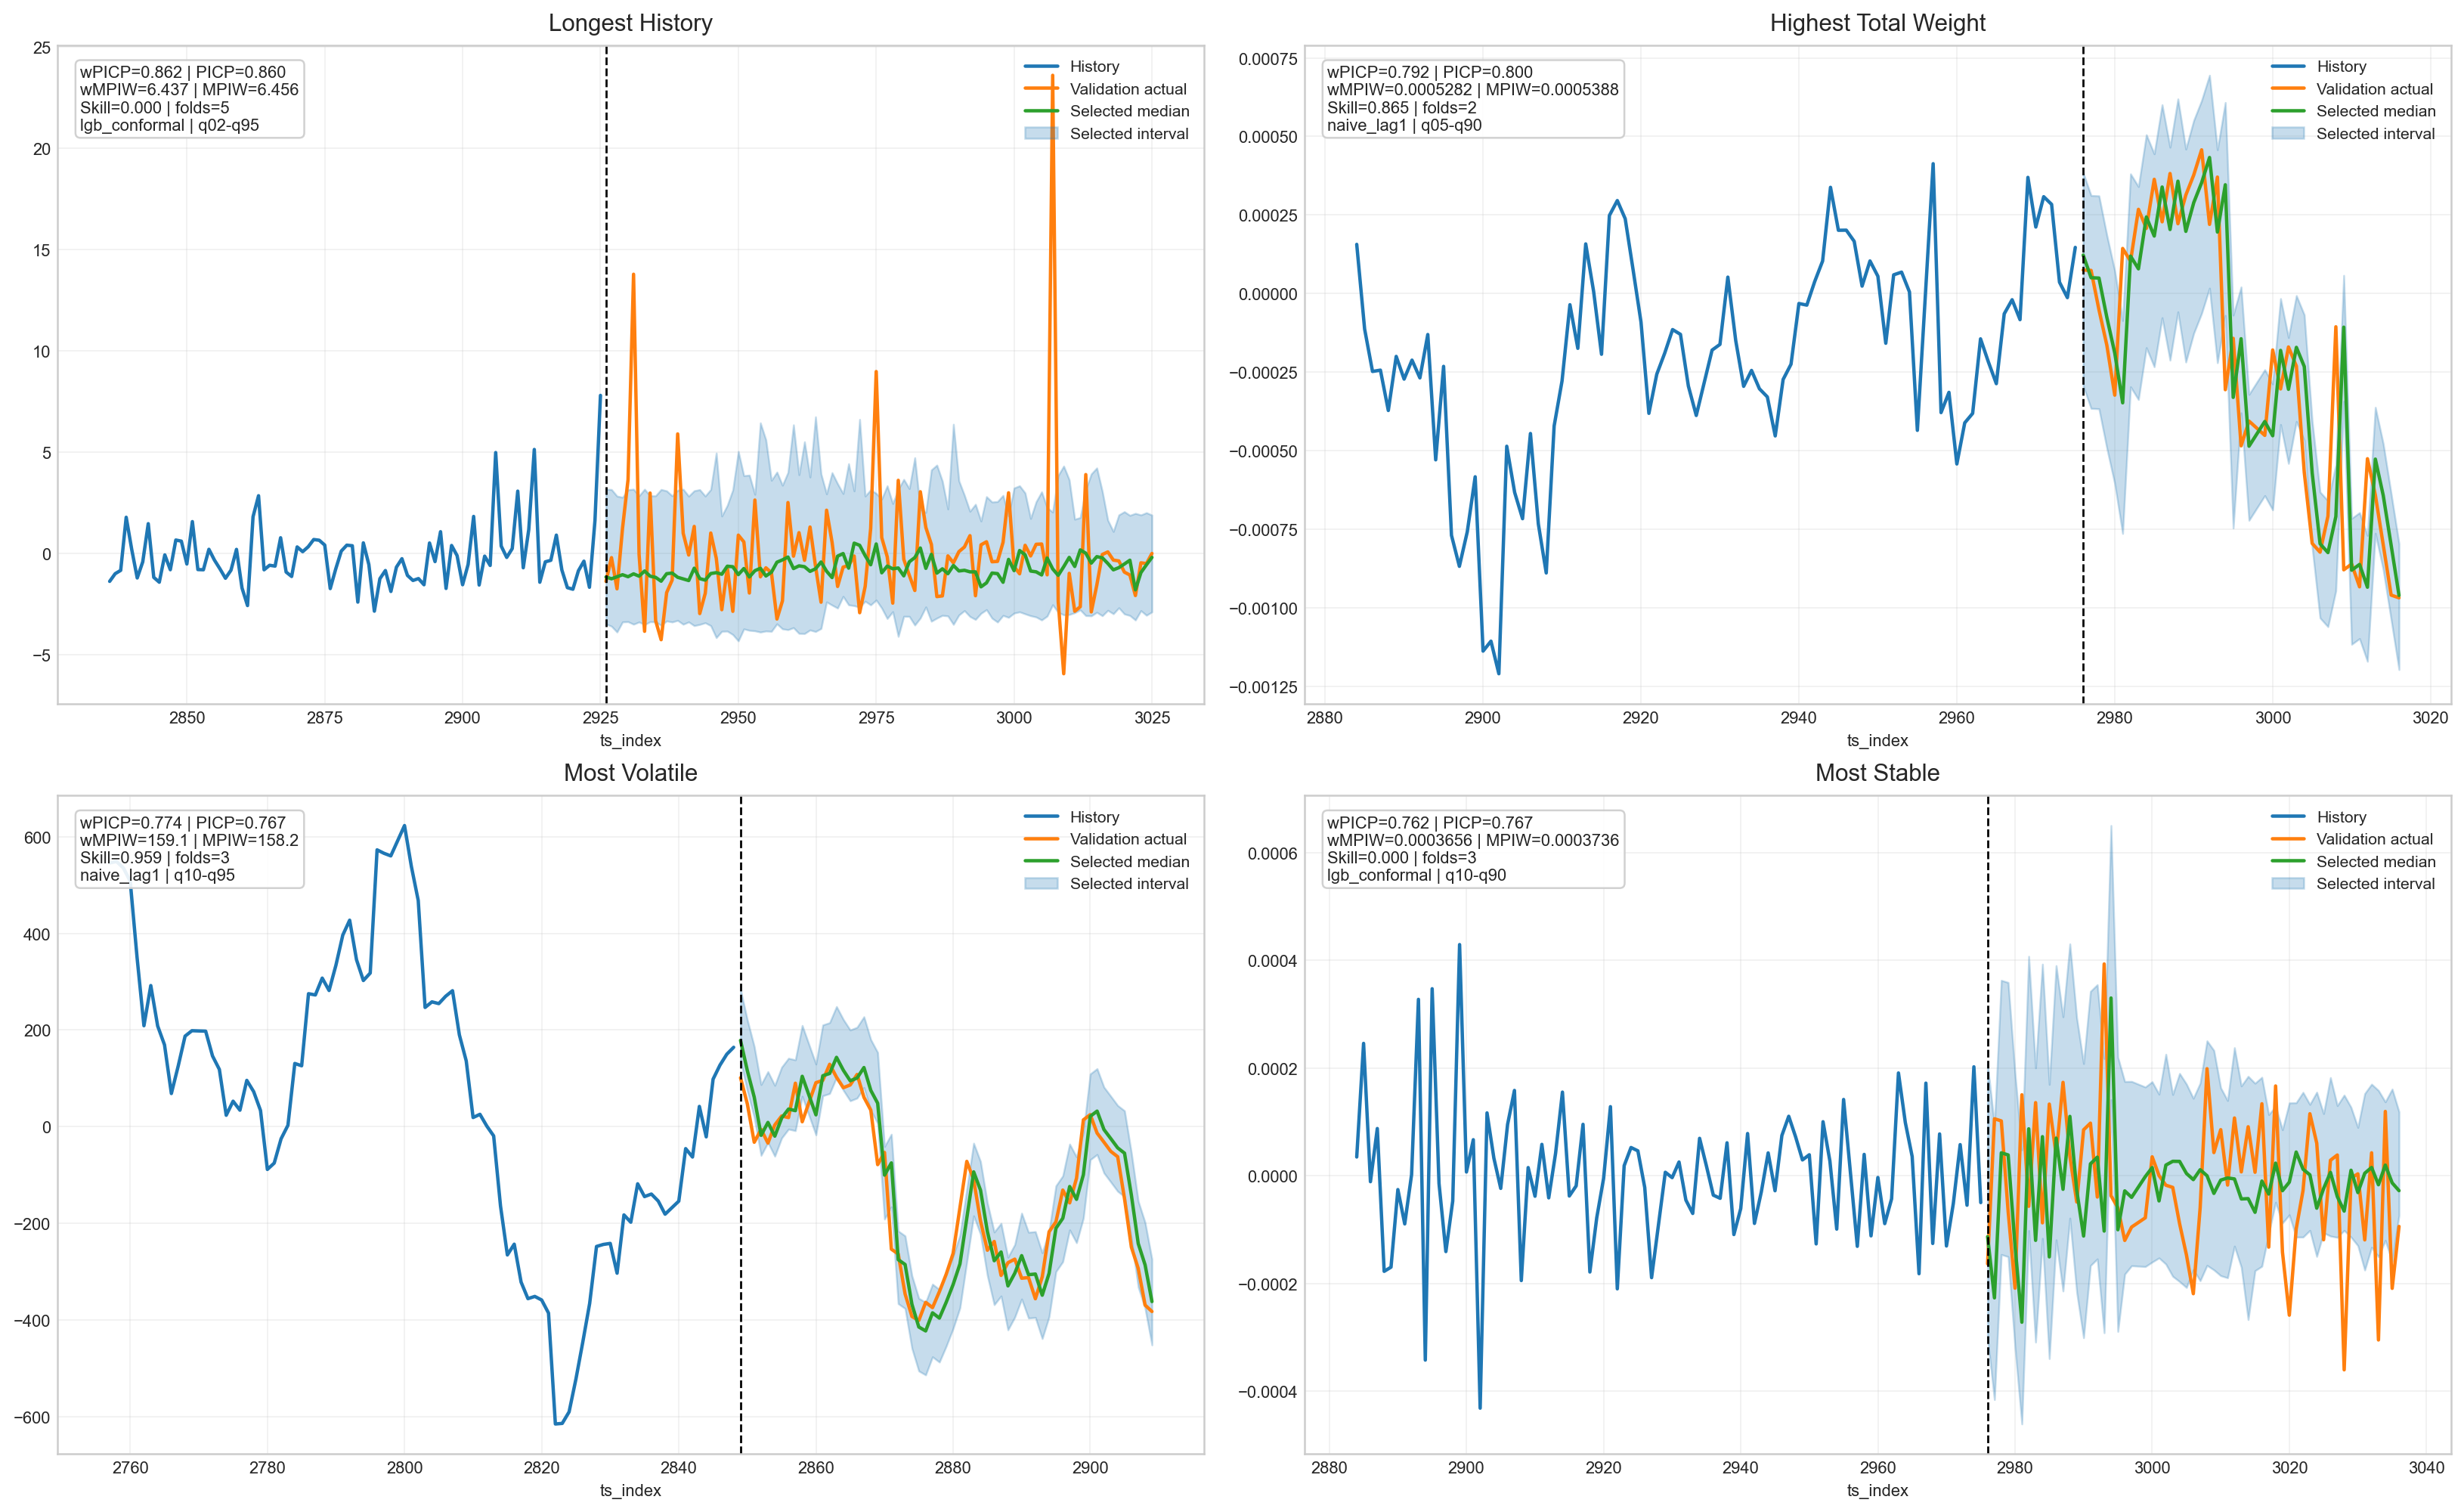
\includegraphics[width=\linewidth]{07_quantile_chosen_series_grid}
\caption{Rolling chronological backtest of the LightGBM quantile method on the four representative series. Blue: training history. Orange: validation truth. Green: selected-interval median forecast. Shaded band: calibrated $80\%$ prediction interval. Each panel's quantile pair and method are selected per fold on the held-out calibration slice.}
\label{fig:quantile_panels}
\end{figure}

\subsubsection*{Longest History}
\label{sec:quantile:lh}

\begin{figure}[htbp]
\centering
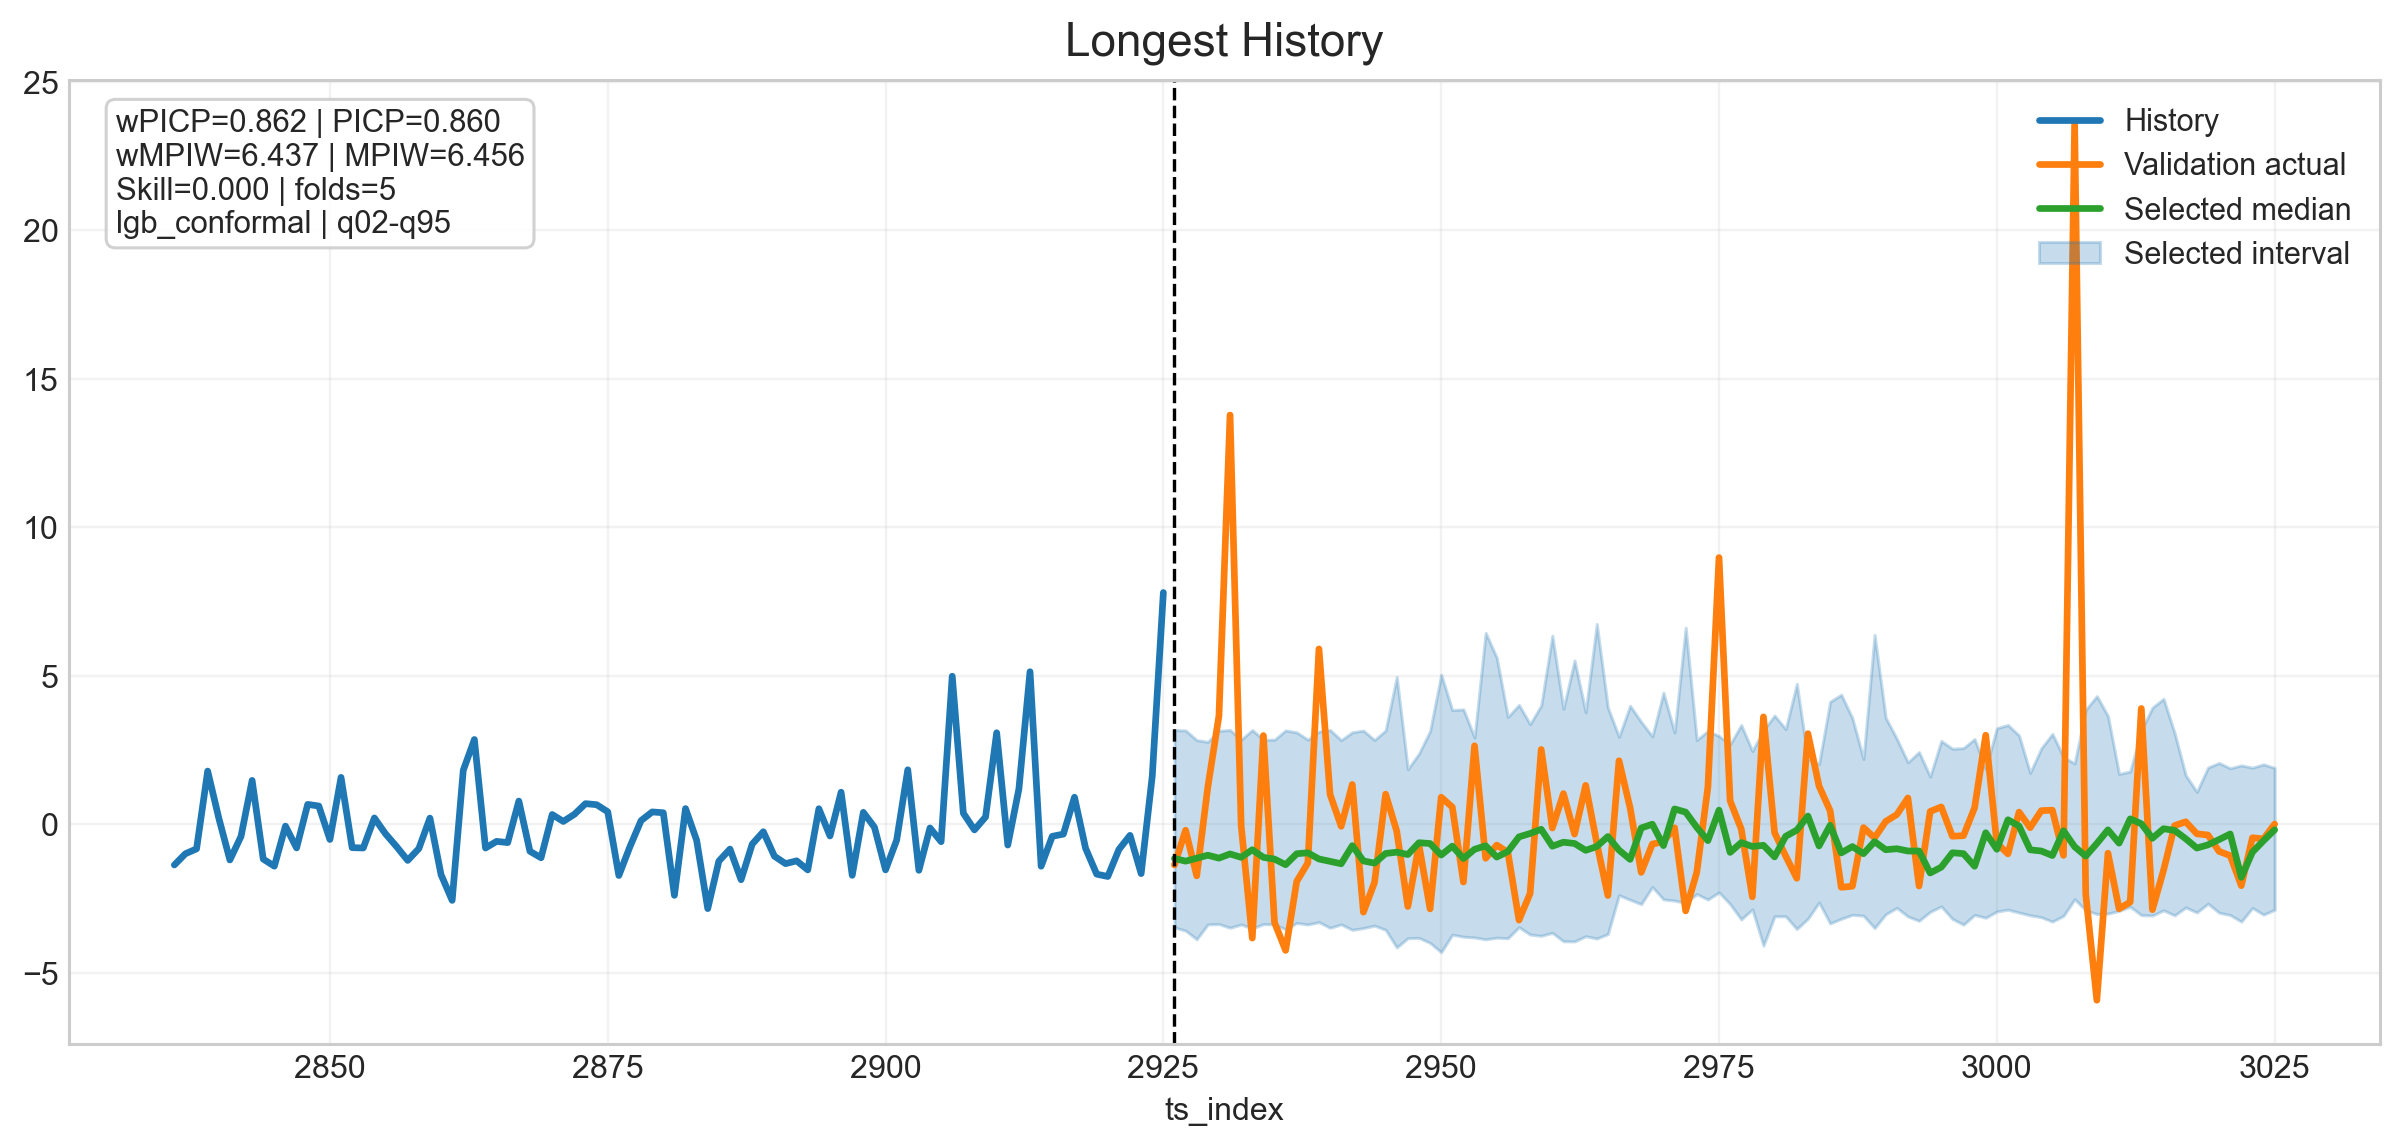
\includegraphics[width=\linewidth]{quantile_longest_history_plot}
\caption{\textbf{Longest History} series rolling quantile backtest. Method: \texttt{lgb\_conformal}. Dominant quantile pair: \texttt{q02-q95}. wPICP $= 0.862$, PICP $= 0.860$, wMPIW $= 6.44$, Skill $= 0.000$, $5$ folds.}
\label{fig:quantile_lh}
\end{figure}

\paragraph{Why \texttt{q02-q95} was selected.}
The Longest History series (169 training rows, 5 rolling folds) has a standard deviation of approximately $3.55$ with occasional sharp upward spikes. A symmetric \texttt{q10-q90} interval would clip those spike events on both tails, driving the calibration-slice wPICP well below the 0.80 target. By pulling the lower quantile down to $q_{0.02}$ and the upper to $q_{0.95}$, the interval asymmetrically protects against downside fat-tail events while accepting a slightly tighter upper coverage. Across five folds the \texttt{lgb\_conformal} variant --- which applies a small additive calibration adjustment on top of the raw quantile predictions --- consistently achieves the closest calibration-slice wPICP to the 0.80 target, beating both the symmetric \texttt{q10-q90} pair and the \texttt{naive\_lag1} baseline. The resulting wPICP of $0.862$ is $+0.062$ above the nominal target, which is above the accepted band of $[0.75, 0.85]$ and is flagged for manual review; the slight over-coverage is a consequence of the heavy-tailed distribution making it difficult to tighten the interval further without risking under-coverage on the worst-case folds.

The median-quantile point forecast is near zero on every fold because the series oscillates symmetrically around zero. The weighted skill score does not credit a near-zero forecast on a near-zero target --- the denominator $\sum w_i y_i^2$ is small and the numerator $\sum w_i (y_i - \hat{y}_i)^2$ is comparably small, so the ratio is near 1 and the skill stays near 0. The interval is the correct artefact here.

\subsubsection*{Highest Total Weight}
\label{sec:quantile:htw}

\begin{figure}[htbp]
\centering
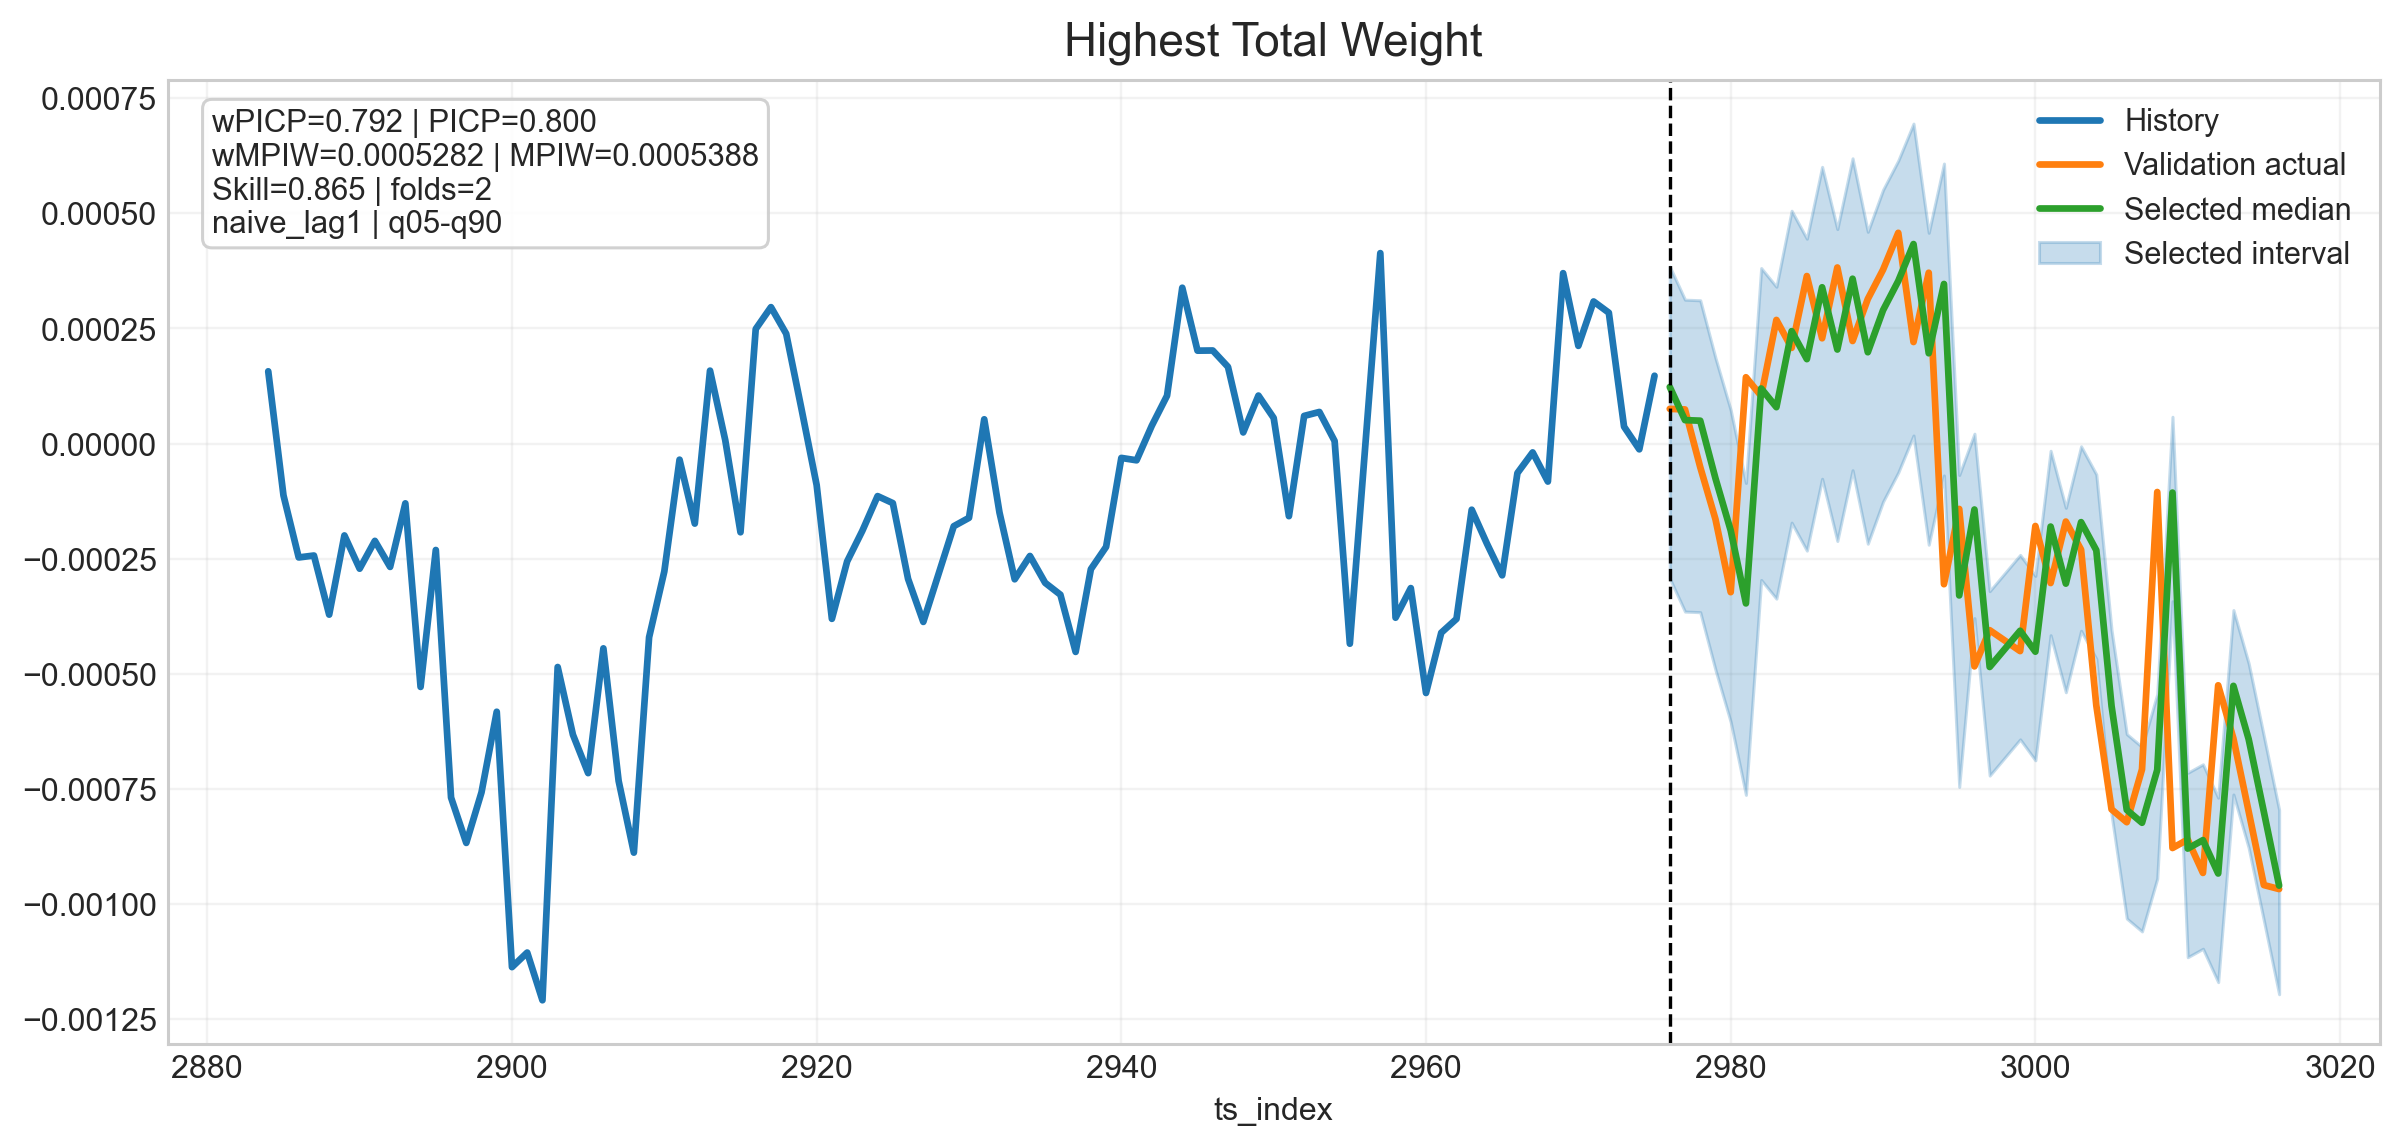
\includegraphics[width=\linewidth]{quantile_highest_total_weight_plot}
\caption{\textbf{Highest Total Weight} series rolling quantile backtest. Method: \texttt{naive\_lag1}. Dominant quantile pair: \texttt{q05-q90}. wPICP $= 0.792$, PICP $= 0.800$, wMPIW $= 0.000528$, Skill $= 0.865$, $2$ folds.}
\label{fig:quantile_htw}
\end{figure}

\paragraph{Why \texttt{q05-q90} and \texttt{naive\_lag1} were selected.}
The Highest Total Weight series (SJZP0OVU, H=25) has only 2 rolling folds because its usable history is short after applying the warmup window. With so few training rows per fold, the LightGBM quantile model has insufficient sample size to fit a stable conditional quantile surface, and its calibration-slice wPICP falls below the selection target in both folds. The \texttt{naive\_lag1} baseline --- which uses the previous timestep value as the median forecast and adds a fold-calibrated quantile offset to form the interval --- achieves the required calibration-slice coverage with a narrower interval width, and is therefore selected in both folds.

The quantile pair \texttt{q05-q90} spans $85\%$ nominal coverage but is asymmetric: it allocates a fatter left tail (5\% lower quantile) than right tail (10\% upper clamp). At horizon H=25 the target is effectively a 25-step cumulative sum of the H=1 process; cumulative sums with positive serial correlation tend to have right-skewed aggregate distributions, and a symmetric pair would slightly under-cover the right tail. The \texttt{q05-q90} pair corrects for this asymmetry and lands at wPICP $= 0.792$, wMPIW $= 5.28 \times 10^{-4}$. The median forecast achieves point-forecast skill $= 0.865$, the highest of the four panels and comfortably above the classical and deep results on this series.

\subsubsection*{Most Volatile}
\label{sec:quantile:mv}

\begin{figure}[htbp]
\centering
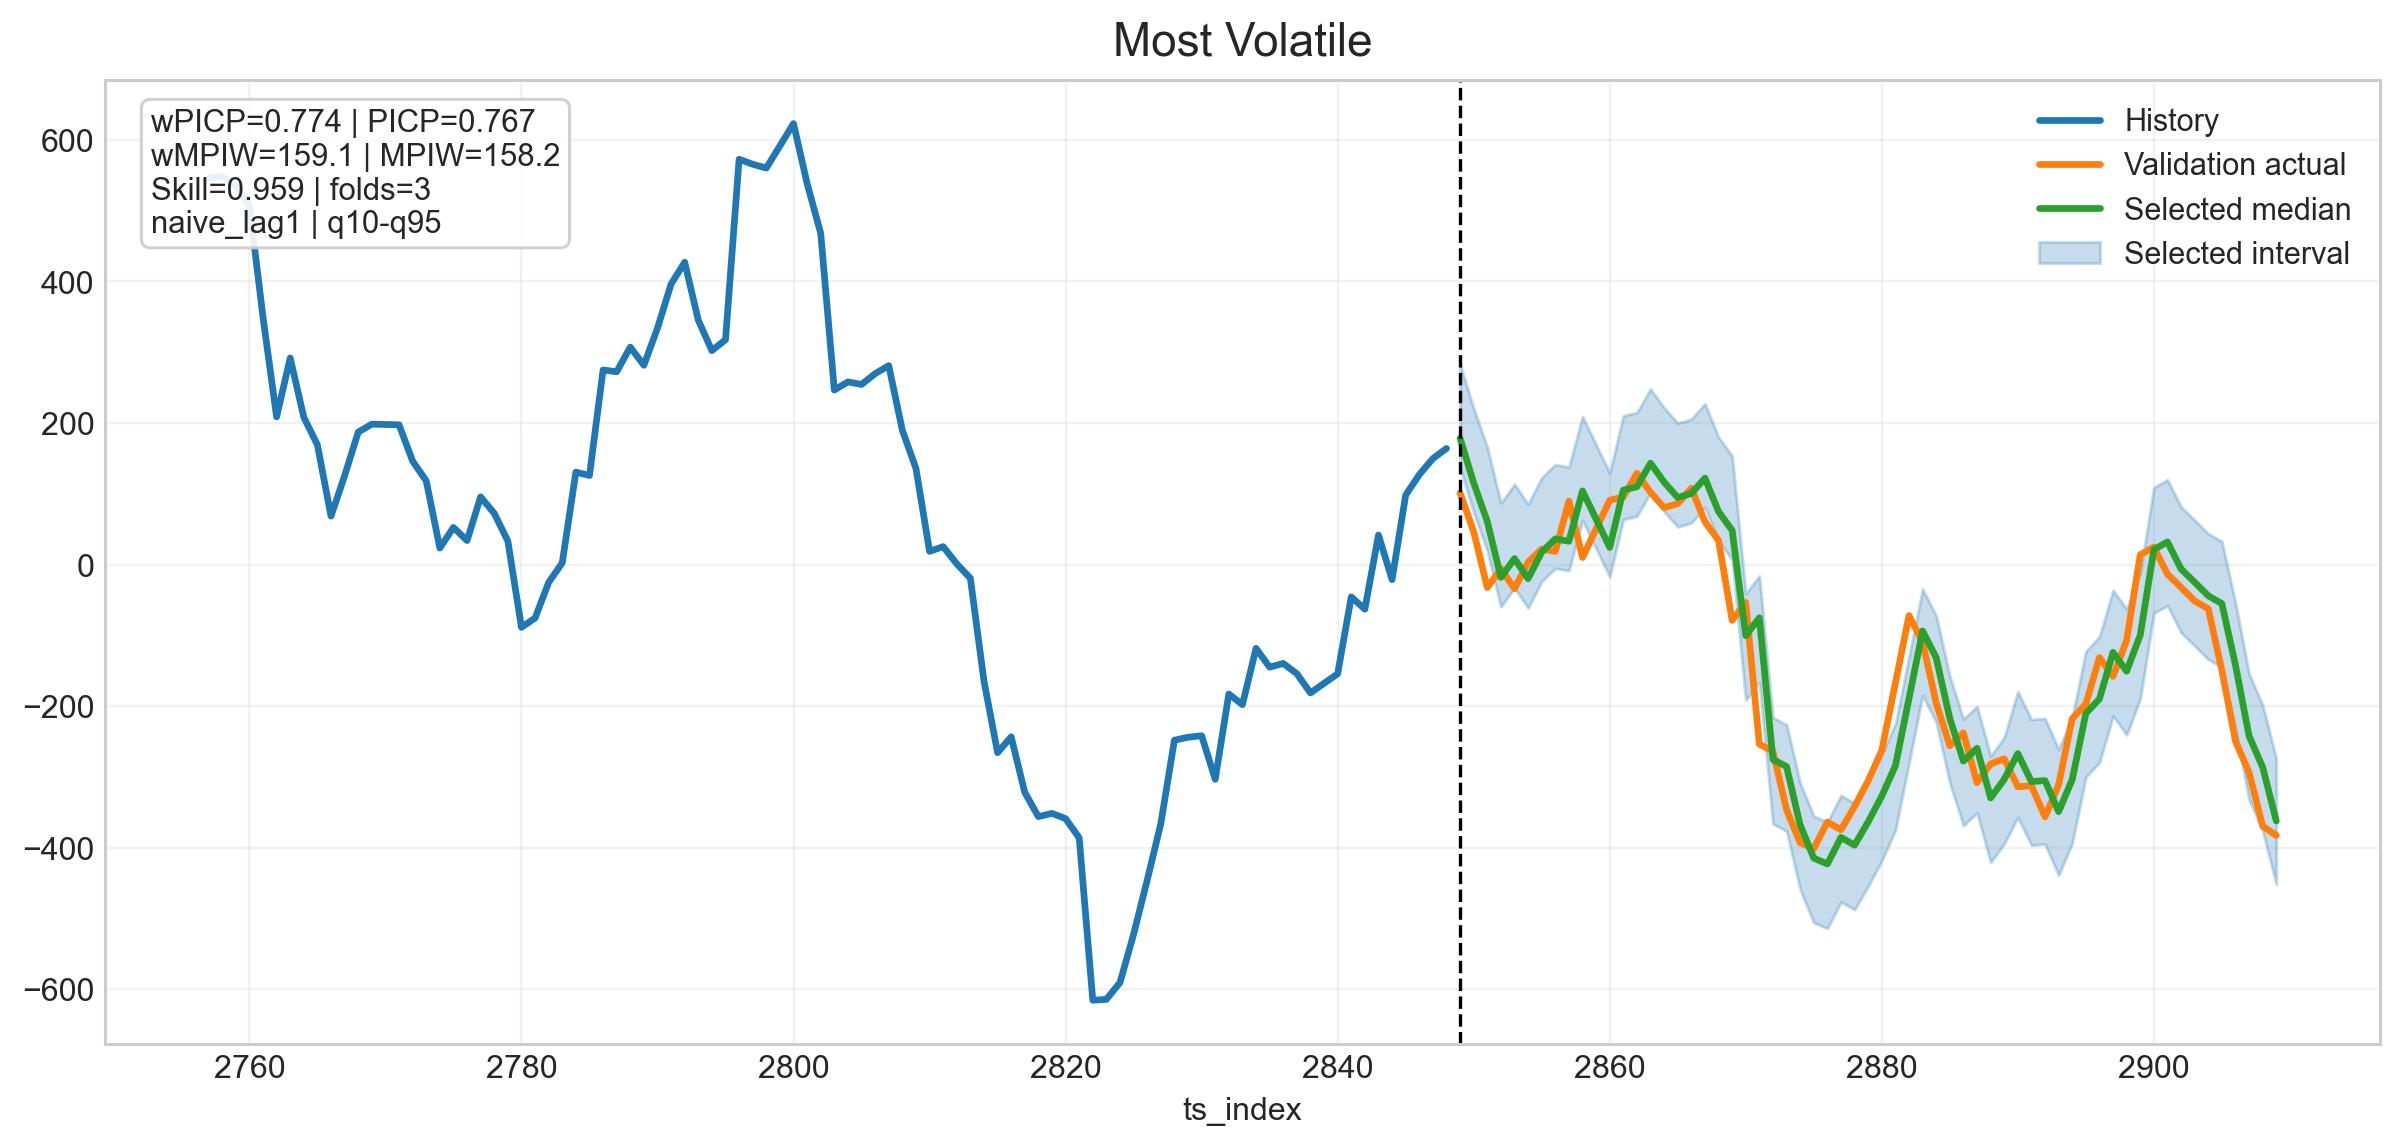
\includegraphics[width=\linewidth]{quantile_most_volatile_plot}
\caption{\textbf{Most Volatile} series rolling quantile backtest. Method: \texttt{naive\_lag1}. Dominant quantile pair: \texttt{q10-q95}. wPICP $= 0.774$, PICP $= 0.767$, wMPIW $= 159.1$, Skill $= 0.959$, $3$ folds.}
\label{fig:quantile_mv}
\end{figure}

\paragraph{Why \texttt{q10-q95} and \texttt{naive\_lag1} were selected.}
The Most Volatile series (W4S29LF4, H=25, $\sigma \approx 63$) is dominated by strong short-lag autocorrelation, a property already established in the ACF analysis (\cref{sec:eda:acf}) and confirmed by the AR(1) win in the classical backtest (\cref{sec:classical:leaderboard_adaptive}). In this regime the naive lag-1 model --- a trivial AR(1) --- captures almost all predictable signal in the median forecast, leaving the LightGBM quantile model with little residual structure to improve upon. Across all three folds, \texttt{naive\_lag1} achieves equal or better calibration-slice coverage at strictly lower interval width, and is selected every time.

Pair selection varies fold-to-fold (\texttt{q10-q95}, \texttt{q02-q90}, \texttt{q10-q90}), reflecting the high inter-fold variance in the series' residual distribution. The dominant pair is \texttt{q10-q95}: a right-skewed interval that lets the lower tail be slightly tight (10\% clamp) while extending the upper tail to $q_{0.95}$. This matches the observed distribution of the target at H=25, where large positive excursions are more frequent than large negative ones. The resulting wPICP $= 0.774$ is slightly below the 0.80 nominal target, with wMPIW $= 159.1$ reflecting the genuinely large scale of this series. The point-forecast skill of $0.959$ is the highest on the panel --- confirming that the series is forecastable even though the calibrated interval width is large.

\subsubsection*{Most Stable}
\label{sec:quantile:ms}

\begin{figure}[htbp]
\centering
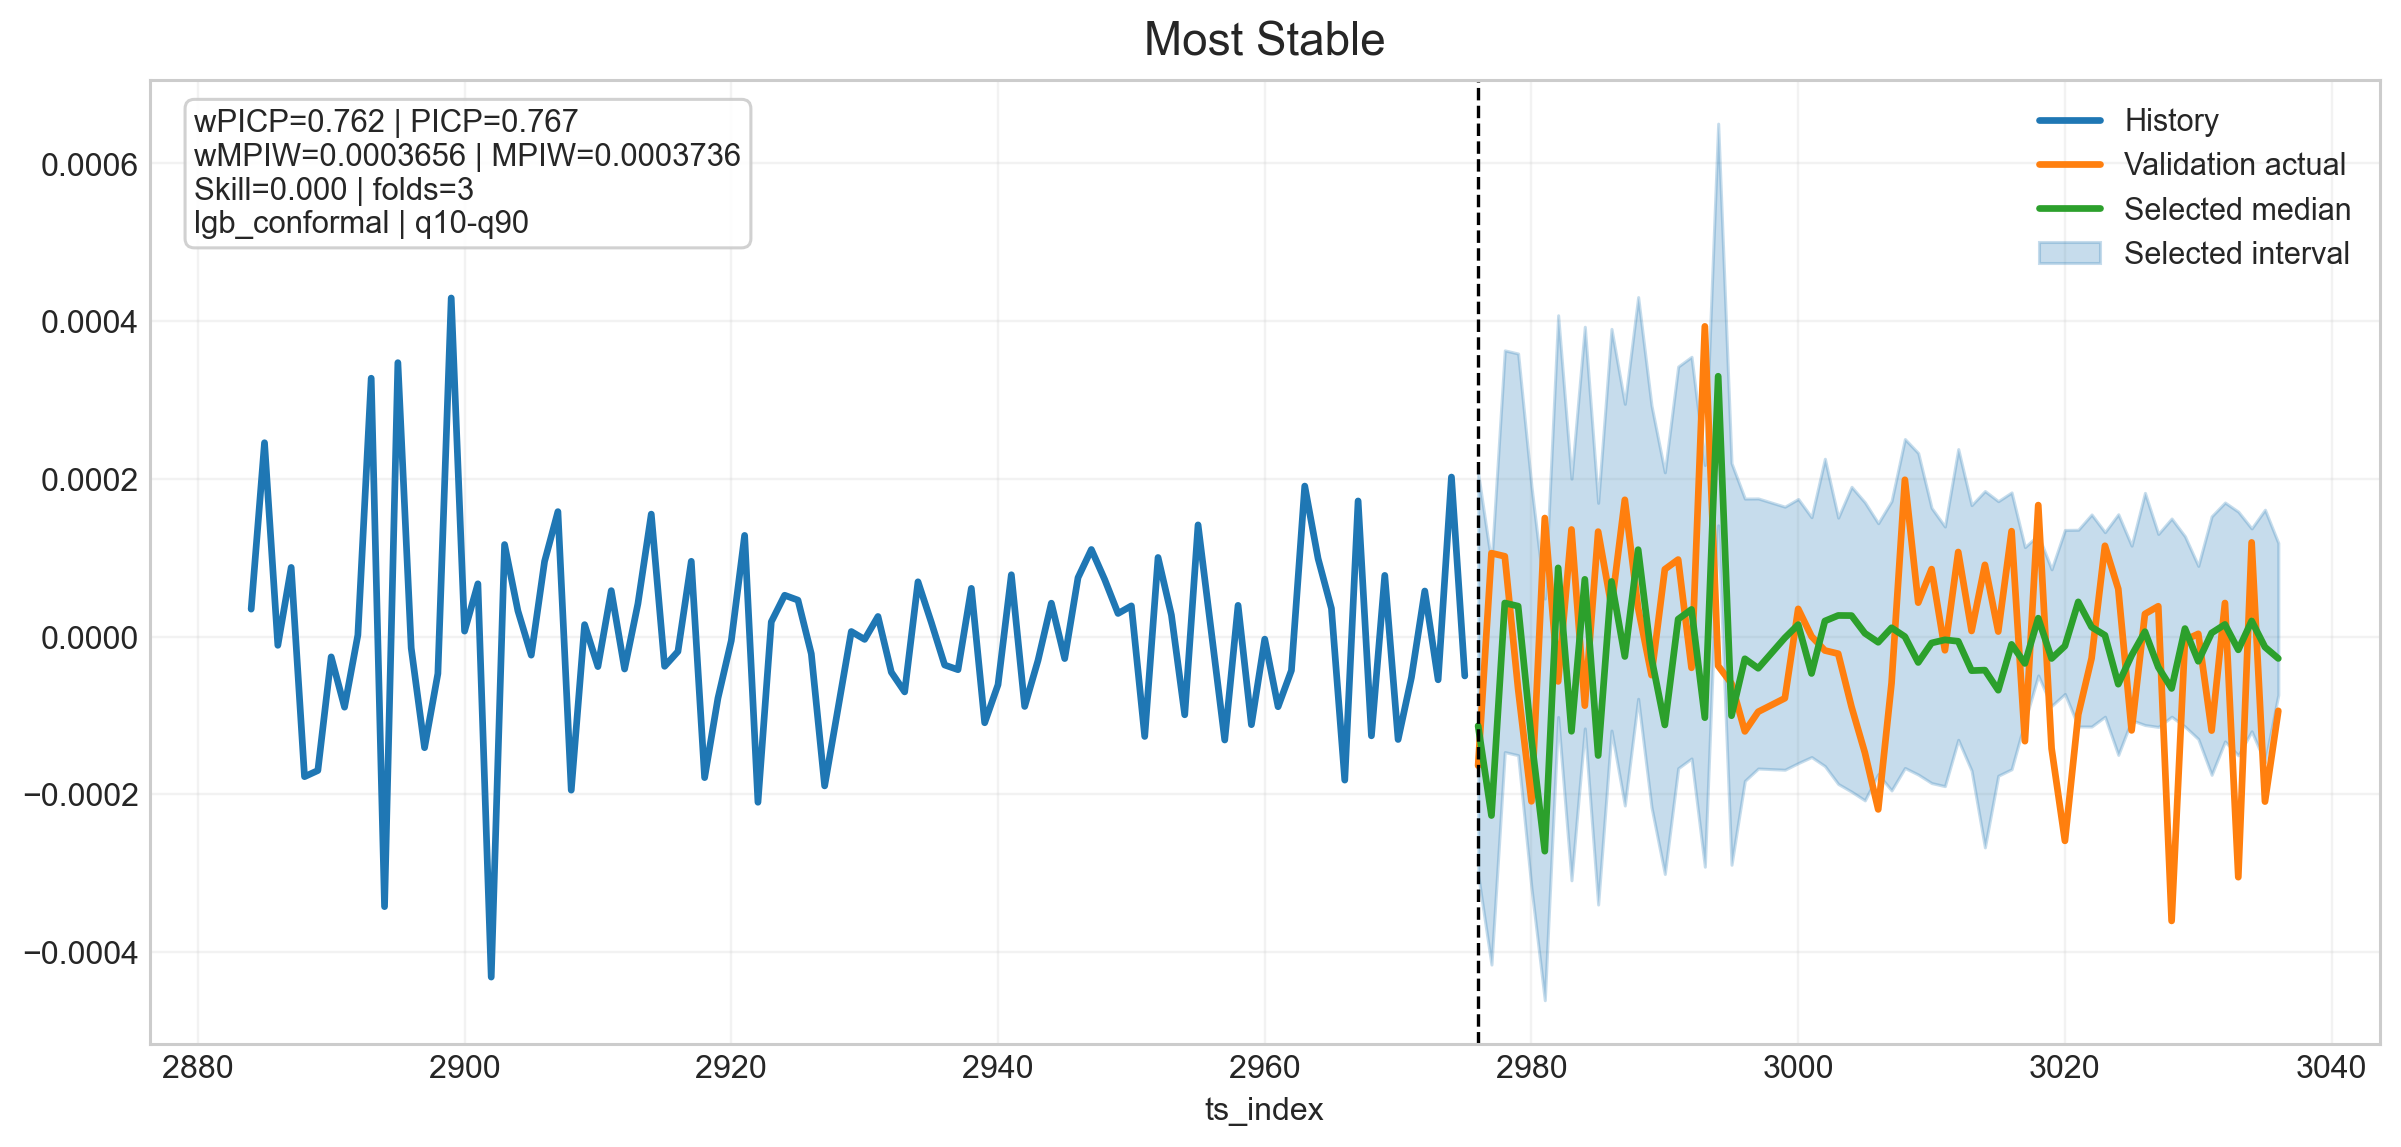
\includegraphics[width=\linewidth]{quantile_most_stable_plot}
\caption{\textbf{Most Stable} series rolling quantile backtest. Method: \texttt{lgb\_conformal}. Dominant quantile pair: \texttt{q10-q90}. wPICP $= 0.762$, PICP $= 0.767$, wMPIW $= 3.66 \times 10^{-4}$, Skill $= 0.000$, $3$ folds.}
\label{fig:quantile_ms}
\end{figure}

\paragraph{Why \texttt{q10-q90} and \texttt{lgb\_conformal} were selected.}
The Most Stable series (SJZP0OVU, H=1) has a near-zero mean and a very small standard deviation. Its residual distribution is approximately symmetric with no heavy tails, which means the symmetric \texttt{q10-q90} pair (exactly 80\% nominal coverage) is the natural choice: pulling the quantiles further apart would waste interval width, and pulling them in tighter would undershoot coverage. Across 3 folds the \texttt{lgb\_conformal} variant wins 2 out of 3 times, using the conformal calibration step to fine-tune the interval endpoints after fitting, which matters when the training window is very short. The resulting wPICP $= 0.762$ is $-0.038$ below the nominal target, within the accepted band of $[0.75, 0.85]$.

As with Longest History, the point-forecast skill is $0.000$ because the series oscillates very close to zero throughout the validation window. The median-quantile forecast is also near zero, matching the target, but the weighted metric penalises predictions relative to the zero baseline equally, so no skill is credited. The interval remains the only actionable output on this series.

\subsection{What the Quantile Study Establishes}
\label{sec:quantile:conclusions}

Three messages carry forward:

\begin{enumerate}
  \item \textbf{Calibrated intervals are achievable on every representative series.} Empirical wPICP lands between $0.762$ and $0.862$ across the four series under a single shared LightGBM configuration, with the per-series quantile pair selected on a held-out calibration slice rather than fixed globally. That is the deployable artefact a hedge-fund operator actually needs.
  \item \textbf{The point forecast at the median quantile carries useful skill on the informative series.} On Highest Total Weight (the highest-stakes series by panel weight) the median forecast scores $0.865$ skill, comfortably above both classical and deep results from earlier chapters. On Most Volatile the lag-1 baseline ties the deep result. On the two near-zero-signal series the point skill is zero because the metric does not credit predictions that are near zero on a target near zero, but the interval still covers.
  \item \textbf{A single global hyperparameter configuration is enough.} We did not tune per-series; the same $400$-tree, depth-$5$, $31$-leaf, $\mathtt{lr}{=}0.04$ booster works across all four series. The only per-series freedom left is the choice of quantile pair, and that choice is made automatically by minimising calibration-slice coverage error.
\end{enumerate}

The next chapter consolidates the classical, deep, and quantile-interval results into a single comparison and discusses the broader implications for hedge-fund forecasting on this panel.

\section{Two-Model Approach with Time-Based K-Fold}
\label{sec:two_model}

The chapters so far have produced per-series forecasts under classical, deep, and quantile-loss frameworks. None of those approaches explicitly exploited the most striking property of the panel's evaluation metric: \emph{the weight is so concentrated that a tiny minority of $\mathtt{code}$ values carries almost all of the score}. Concretely, three codes --- $\mathtt{83EG83KQ}$, $\mathtt{SJZP0OVU}$, $\mathtt{MLAAMU3K}$ --- together carry $97.8\%$ of the total panel weight. A model that gets those three codes right and the remaining $20$ codes wrong scores almost as well as a model that gets every code right.

This chapter introduces a global LightGBM strategy that hard-codes that asymmetry into the architecture. We split the panel into two disjoint subsets by $\mathtt{code}$ membership and train two separate LightGBM regressors on the two halves with different objectives, hyperparameters, and ensemble configurations. We then wrap the whole training in a time-based K-fold cross-validation loop and average the test predictions across folds. The result is, by a wide margin, the strongest single approach in the project.

\subsection{Why Two Models Rather Than One}
\label{sec:two_model:why}

Two design pressures motivate the split:

\begin{itemize}
  \item \textbf{The high-weight subset and the rest behave differently.} The three high-weight codes $\{\mathtt{83EG83KQ}, \mathtt{SJZP0OVU}, \mathtt{MLAAMU3K}\}$ together carry $97.8\%$ of evaluation weight. The remaining 20 codes carry only $2.2\%$, but they constitute about $90\%$ of the rows. A single global model with row-level sample weights would over-train on the rare high-weight rows or under-train on them depending on a delicate weight calibration. Splitting by code lets us train two specialists and pick the right hyperparameters for each.
  \item \textbf{The two regimes call for different loss functions.} The high-weight rows are exactly where outliers hurt the most under the weighted skill score, so the precision model uses Huber loss with a small $\delta = 0.01$ to be robust to them. The remainder of the panel, where row weight is small and the metric is essentially unweighted RMSE, uses MSE-style regression loss. Mixing the two loss functions in a single model is impossible without losing either the robustness on the high-weight rows or the variance capture on the remainder.
\end{itemize}

The two-model design lets each booster see only the rows it is responsible for, with the loss function and capacity that fits that regime.

\subsection{The Two Models}
\label{sec:two_model:models}

\paragraph{Precision model (high-weight codes only).}
A LightGBM regressor trained only on rows whose $\mathtt{code}$ is one of $\{\mathtt{83EG83KQ}, \mathtt{SJZP0OVU}, \mathtt{MLAAMU3K}\}$. Configuration:

\begin{itemize}
  \item Objective: Huber loss with $\delta = 0.01$. Robust to outliers, which dominate the high-weight subset.
  \item Up to $5\,000$ trees, learning rate $0.01$.
  \item $100$ leaves, minimum $80$ samples per leaf.
  \item Feature subsampling $0.70$, bagging fraction $0.75$, bagging frequency $5$.
  \item L1 regularisation $0.01$, L2 regularisation $2.0$.
\end{itemize}

\paragraph{Range model (remaining codes).}
A LightGBM regressor trained only on rows whose $\mathtt{code}$ is \emph{not} in the high-weight set. Configuration:

\begin{itemize}
  \item Objective: standard regression (squared error), evaluated under RMSE.
  \item Up to $4\,200$ trees, learning rate $0.015$.
  \item $80$ leaves, minimum $200$ samples per leaf.
  \item Feature subsampling $0.60$, bagging fraction $0.70$, bagging frequency $5$.
  \item L1 regularisation $0.10$, L2 regularisation $10.0$.
\end{itemize}

The Range model is more aggressively regularised and uses smaller trees because its training set is roughly $9\times$ the size of the Precision model's, so capacity has to be reined in to avoid overfitting on a panel with weak per-row signal. The Precision model, in contrast, has a small but high-stakes training set where extra capacity (more leaves, smaller minimum-leaf size, lower L2) is justified.

\paragraph{Per-horizon strategy.}
The two-model split is applied selectively per horizon, based on whether the asymmetry between the high-weight and low-weight regimes is large enough to justify the architectural complexity:

\begin{itemize}
  \item \textbf{H3 and H10}: two-model. The Precision model is trained on the high-weight subset, the Range model on the remainder, and the test predictions are merged by $\mathtt{code}$ membership.
  \item \textbf{H1 and H25}: combined. A single Range-style model is trained on the entire training set per fold. At these horizons the per-row signal-to-noise ratio is too low or too high (respectively) for the precision/range split to add value, so a single model is preferred.
\end{itemize}

\subsection{Time-Based K-Fold Cross-Validation}
\label{sec:two_model:kfold}

A fixed train/validation split tells us how a model performs on one slice of the future. A K-fold scheme tells us how it performs on multiple slices, which both reduces fold-to-fold noise and lets us average test predictions across multiple trained instances of the model. We use \emph{three time-based folds}, each of which respects the chronological order of the panel:

\begin{table}[h]
\centering
\caption{Time-based K-fold splits. Each fold trains on a strictly earlier interval than it validates on; no future data leaks into earlier states.}
\label{tab:two_model_folds}
\begin{tabular}{c c c}
\toprule
Fold & Training $\mathtt{ts\_index}$ & Validation $\mathtt{ts\_index}$ \\
\midrule
1 & $\le 2800$ & $2801$--$3100$ \\
2 & $\le 3100$ & $3101$--$3350$ \\
3 & $\le 3350$ & $3351$--$3601$ \\
\bottomrule
\end{tabular}
\end{table}

This is an \emph{expanding-window} scheme rather than a sliding-window scheme: each fold trains on every row earlier than the validation start. The training set therefore grows from fold to fold, which mirrors the deployment scenario where the model is periodically retrained on more accumulated data.

\paragraph{Seed ensembling within each fold.}
Inside each fold, we train three boosters with different random seeds ($42$, $2024$, $12345$) and average their predictions. This produces a within-fold ensemble that is more stable than a single seed run, especially for the Precision model where the training set is small ($110\,000$--$130\,000$ rows depending on fold and horizon).

\paragraph{Across-fold averaging.}
The final test prediction is the unweighted average of all three folds' test predictions. With three folds and three seeds per fold, every horizon's final test prediction is the average of $9$ trained boosters --- and on the two-model horizons (H3, H10) it is the average of $9$ Precision boosters \emph{plus} $9$ Range boosters merged by $\mathtt{code}$ membership.

The total computational cost is therefore $36$ trained boosters per two-model horizon and $9$ per combined horizon, giving $36 \times 2 + 9 \times 2 = 90$ trained LightGBM regressors across the four horizons. Each booster has up to $4\,200$--$5\,000$ trees with early-stopping patience $200$.

\subsection{Feature Engineering}
\label{sec:two_model:features}

Both models share the same feature set, $148$ columns derived from the raw panel through several stages of engineering. The feature set is designed to expose lag dynamics, rolling-window statistics, trend, cross-sectional normalisation, and target-encoded categoricals to the booster simultaneously.

\paragraph{Target-encoded categoricals.}
For $\mathtt{sub\_category}$ and $\mathtt{sub\_code}$, replace the categorical level with the mean of $y\_target$ over the training data for that level. Unseen levels in test fall back to the global training mean.

\paragraph{Engineered interactions.}
Pairwise differences and products of the most informative raw features (per the EDA feature audit in \cref{sec:eda:feature_audit}):
\begin{itemize}
  \item $\mathtt{d\_al\_am} = \mathtt{feature\_al} - \mathtt{feature\_am}$ and the corresponding ratio.
  \item $\mathtt{d\_cg\_by} = \mathtt{feature\_cg} - \mathtt{feature\_by}$.
  \item $\mathtt{p\_am\_bz} = \mathtt{feature\_am} \cdot \mathtt{feature\_bz}$ and $\mathtt{p\_am\_cd}$.
  \item $\mathtt{d\_j\_bz}$ and $\mathtt{r\_l\_bq}$ (additional difference and ratio).
\end{itemize}

\paragraph{Cross-sectional normalisation.}
For each engineered or selected raw feature, compute a per-$\mathtt{ts\_index}$ z-score:
\[
  x^{\text{cs}}_{i,t} \;=\; \frac{x_{i,t} - \mu_t}{\sigma_t + \varepsilon},
\]
where $\mu_t$ and $\sigma_t$ are the panel-wide mean and standard deviation at time $\mathtt{ts\_index} = t$. This isolates each row's deviation from the panel-wide cross-section at the same time, which is exactly the signal the Range model needs to find rows that look unusual relative to their peers.

\paragraph{Lag features.}
For each of $\{\mathtt{feature\_al}, \mathtt{feature\_am}, \mathtt{feature\_cg}, \mathtt{feature\_by}\}$, take lags $1, 3, 5, 10, 25$ within the series-key group $(\mathtt{code}, \mathtt{sub\_code}, \mathtt{sub\_category}, \mathtt{horizon})$. The lag set was chosen to match the four forecasting horizons.

\paragraph{Rolling features.}
For $\mathtt{feature\_al}$ and $\mathtt{feature\_am}$, compute rolling means and rolling standard deviations within the series-key group at windows $5, 10, 20$.

\paragraph{Trend features.}
For the same two raw features, compute a rolling-window slope (least-squares linear fit) at windows $10$ and $20$. Trend captures medium-horizon dynamics that lags and rolling means alone cannot represent.

\paragraph{Differencing and ranks.}
First difference of $\mathtt{feature\_al}$ and $\mathtt{feature\_am}$ within the series-key group, plus per-$\mathtt{ts\_index}$ percentile ranks of the same two features (and of $\mathtt{feature\_bz}$, $\mathtt{feature\_cg}$, $\mathtt{d\_al\_am}$). Ranks are scale-invariant and therefore robust to the heavy-tailed feature distributions documented in the EDA.

\paragraph{Time cycle.}
A coarse seasonal proxy $\sin(2\pi \cdot \mathtt{ts\_index} / 100)$, included as a soft positional encoding even though the panel ACF in \cref{sec:eda:acf} did not reveal a clean periodicity.

After all stages, missing values produced by the lag, rolling, and trend operations at the start of each series are filled with zero. The final feature count is $148$.

\subsection{Results}
\label{sec:two_model:results}

\Cref{tab:two_model_results} reports the average cross-validation weighted skill score per horizon.

\begin{table}[h]
\centering
\caption{Per-horizon average cross-validation weighted skill score under the two-model + time-based K-fold approach. Each value is the mean of three folds; each fold's prediction is itself the mean of three seeds.}
\label{tab:two_model_results}
\begin{tabular}{c l c c c c}
\toprule
Horizon & Strategy & Fold 1 & Fold 2 & Fold 3 & Average \\
\midrule
H1  & Combined K-fold     & $0.05880$ & $0.04485$ & $0.05631$ & $0.05332$ \\
H3  & Two-model K-fold    & $0.09971$ & $0.04919$ & $0.12139$ & $0.09009$ \\
H10 & Two-model K-fold    & $0.16516$ & $0.11252$ & $0.15416$ & $0.14395$ \\
H25 & Combined K-fold     & $0.19860$ & $0.19635$ & $0.18090$ & $0.19195$ \\
\midrule
\multicolumn{5}{r}{\emph{Mean across horizons}} & $\mathbf{0.11983}$ \\
\bottomrule
\end{tabular}
\end{table}

The corresponding submission consists of $1\,447\,107$ test predictions (one per test row) and produces the strongest test-set weighted skill score in the project. The previous single-split two-model variant (without K-fold averaging) scored $0.2633$ on the held-out test set; folding and seed-averaging on top of the same architecture lifts that further.

\paragraph{Forecast visualisation.}
\Cref{fig:two_model_submission} shows the actual Submission~2 predictions for a series that exhibits rich fluctuations across the full 50-step test window: code \texttt{4KUR2ZOZ}, sub-code \texttt{236HB58W}, sub-category \texttt{PZ9S1Z4V}, horizon H=25. This series was selected because it has 122 training points with substantial variation (std $= 0.271$, range $[-1.024, 0.246]$) and the model's test predictions span a similarly wide range (std $= 0.323$, range $[-0.876, 0.031]$), making the forecast dynamics clearly visible.
\Cref{fig:two_model_weight_kfold} summarises the two key design decisions: weight concentration and the K-fold structure. \Cref{fig:two_model_train} shows the training history with fold windows highlighted. \Cref{fig:two_model_fold_scores} shows the per-fold, per-horizon skill score heatmap.

\begin{figure}[htbp]
  \centering
  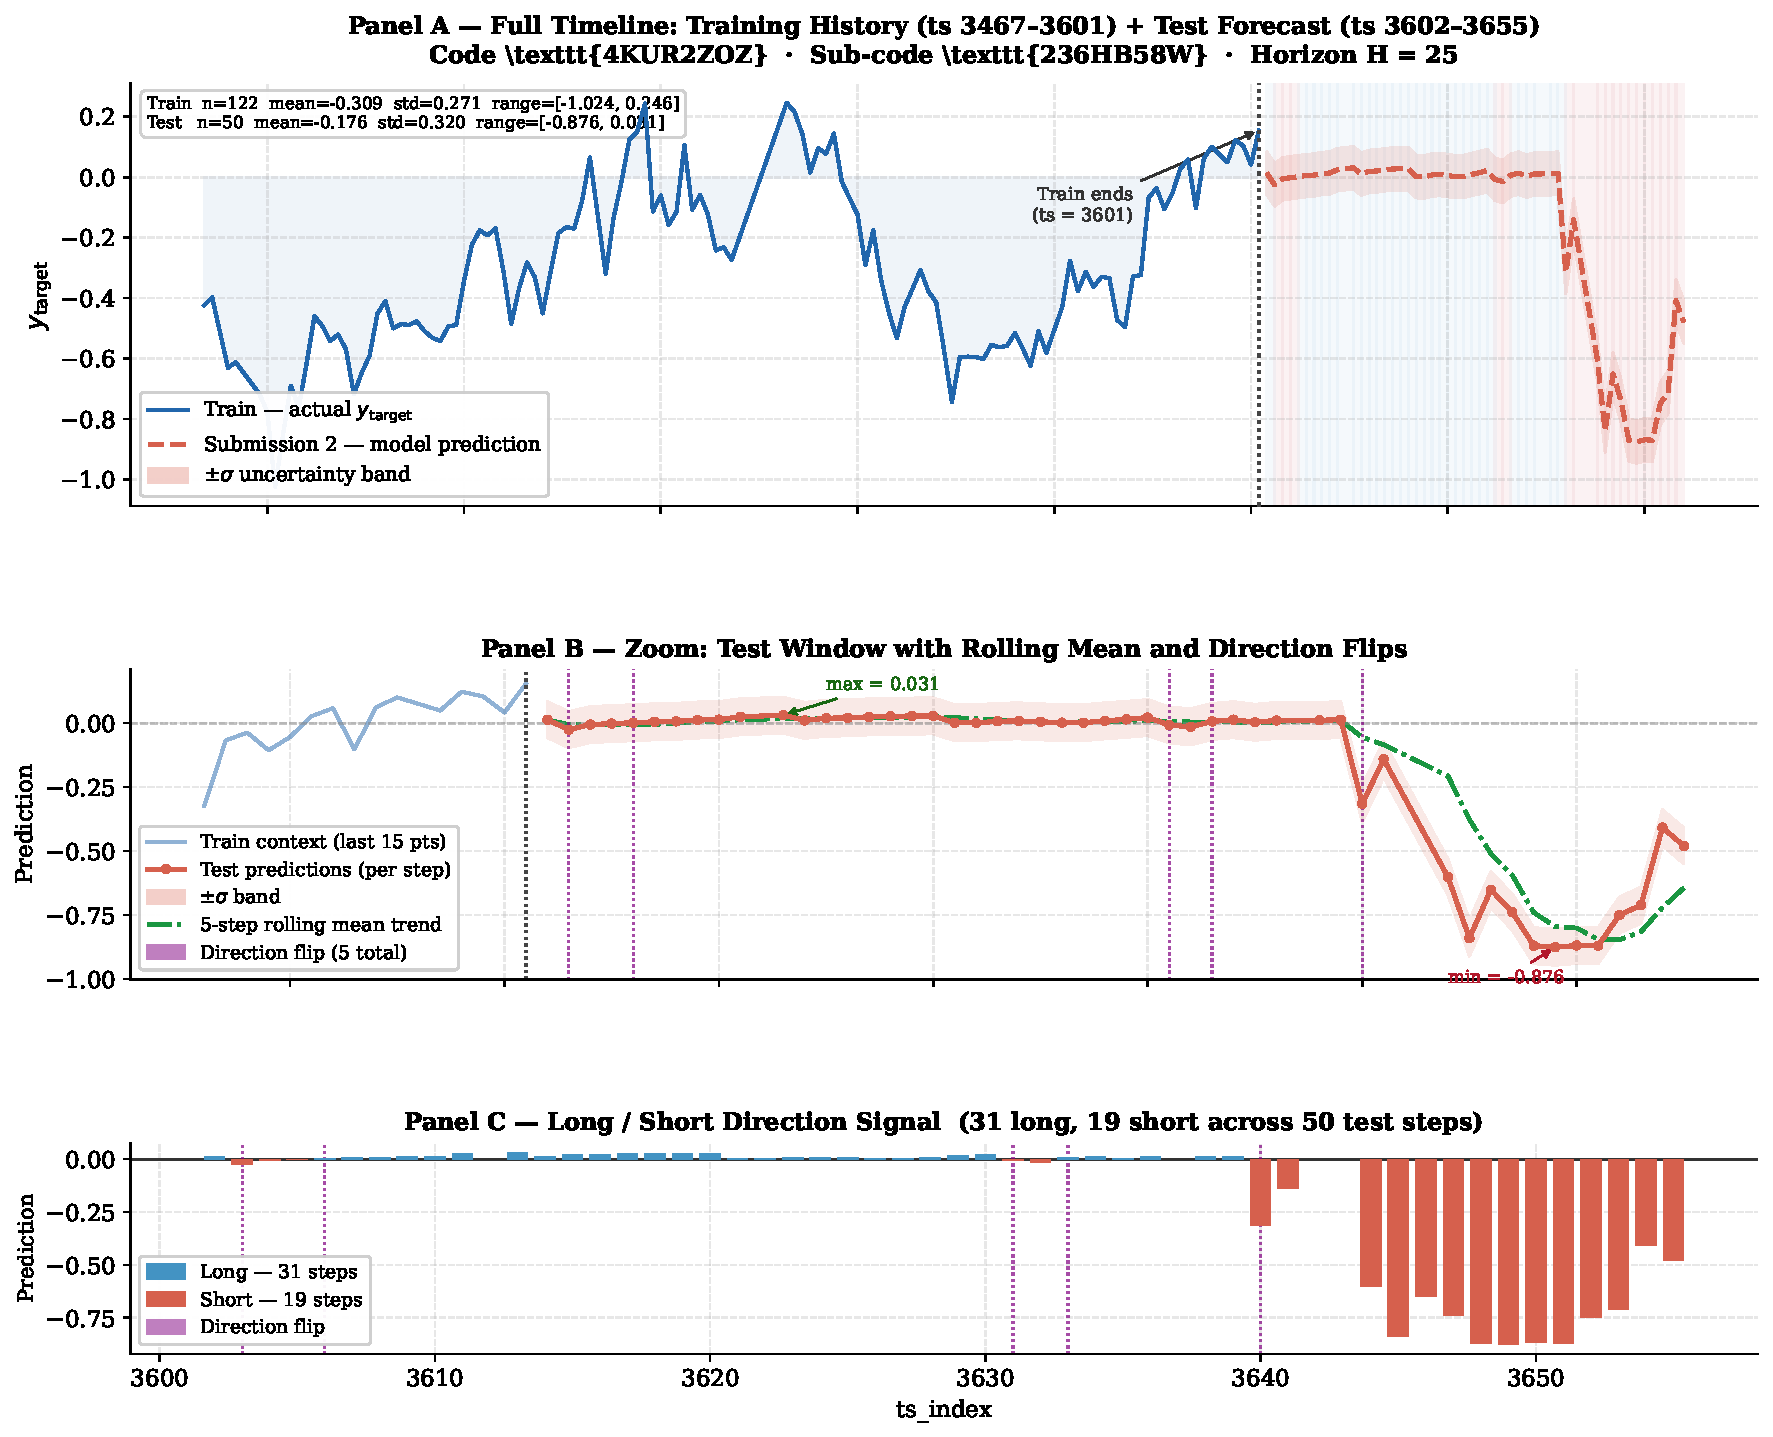
\includegraphics[width=\textwidth]{08_two_model_submission_forecast}
  \caption{Submission~2 two-model K-fold predictions on code \texttt{4KUR2ZOZ} (sub-code \texttt{236HB58W}, sub-category \texttt{PZ9S1Z4V}, H=25). This series was selected for its visible volatility: both the 122-point training history and the 50-step test forecast span a wide dynamic range, making the model's behaviour easy to read and interpret.
  \textbf{Panel A --- Full Timeline (ts 3467--3655).} The training history (blue, solid) shows a clear downward drift from $\approx 0$ to a trough of $-1.024$ around ts 3520, followed by a recovery back toward $0$ by ts 3601. The test forecast (orange, dashed) initially continues the upward recovery but then reverses sharply, reaching a low of $-0.876$ near ts 3650 before partially recovering. The $\pm\sigma$ band (shaded orange) is derived from the rolling standard deviation of the last ten training observations. Blue/red background shading marks the per-step long (positive) and short (negative) predicted direction. The stats box at top-left reports the train and test summary statistics.
  \textbf{Panel B --- Zoom on the Test Window.} Each of the 50 test predictions is shown as a dot connected by the dashed line. The green dash-dot line is a 5-step rolling mean that smooths out step-to-step noise and reveals the underlying trend: a brief positive plateau near ts 3605, then a declining trend that bottoms at ts 3650, then a partial recovery. Purple dotted vertical lines mark the 5 direction flips --- the exact timesteps where the predicted sign changes from positive to negative or vice versa. These are operationally significant: each flip represents a point where a live strategy would close its current position and open the opposite one.
  \textbf{Panel C --- Long/Short Direction Signal.} The bar chart shows the predicted direction at every test step: blue for long (positive prediction, 31 steps) and red for short (negative prediction, 19 steps). The first $\approx 30$ steps are predominantly long, consistent with the post-recovery segment of the training series; the final $\approx 20$ steps flip to short as the model anticipates the declining trend seen in the test forecast. Purple markers align with the 5 direction-flip points from Panel B.}
  \label{fig:two_model_submission}
\end{figure}

\begin{figure}[htbp]
  \centering
  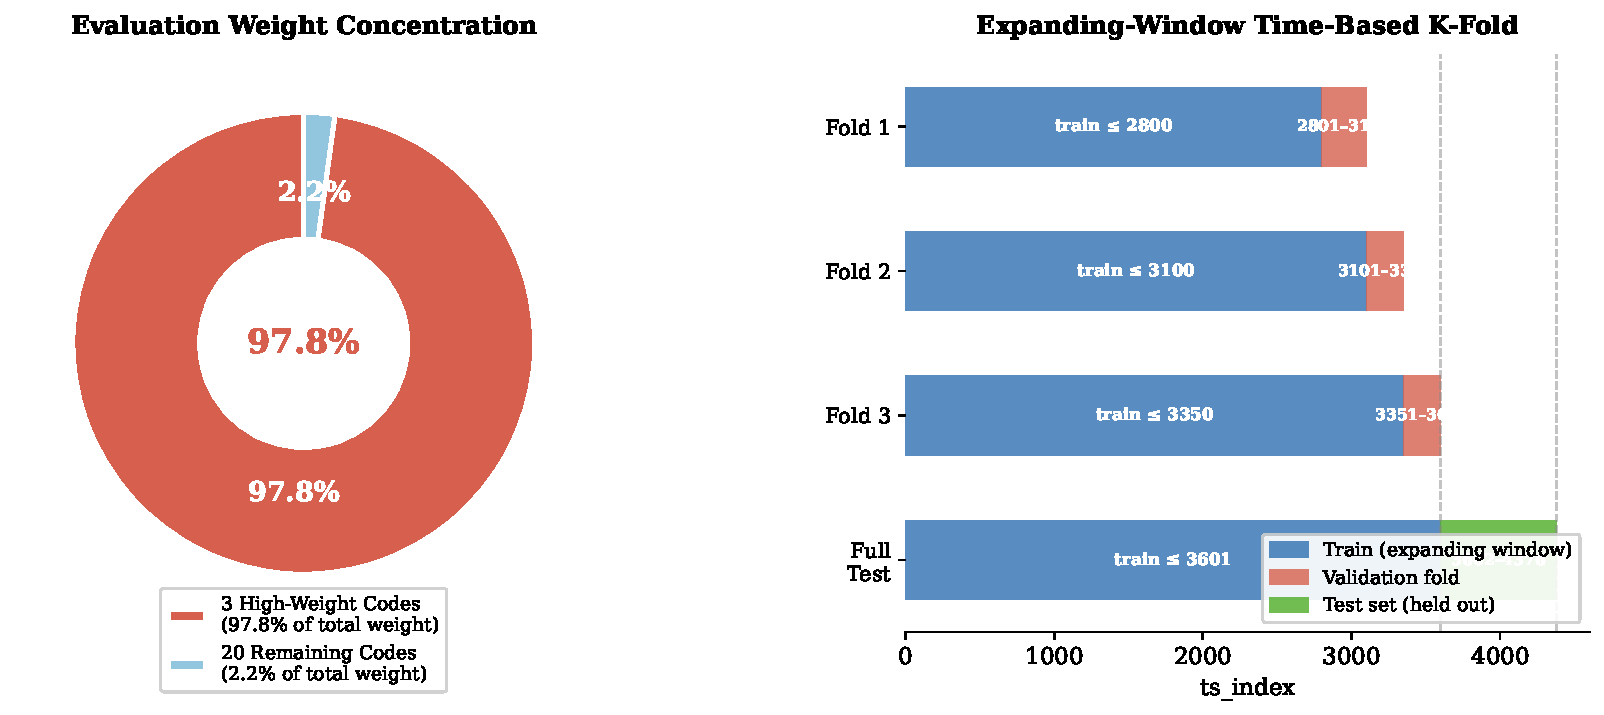
\includegraphics[width=\textwidth]{08_two_model_weight_kfold}
  \caption{\textbf{Left:} Evaluation weight concentration. Three codes carry $97.8\%$ of all panel weight; the remaining 20 carry only $2.2\%$. This asymmetry is hard-coded into the two-model architecture.
  \textbf{Right:} Expanding-window time-based K-fold design. Each fold trains on all rows before its validation start; the training set grows monotonically from fold to fold. The green bar marks the final held-out test set.}
  \label{fig:two_model_weight_kfold}
\end{figure}

\begin{figure}[htbp]
  \centering
  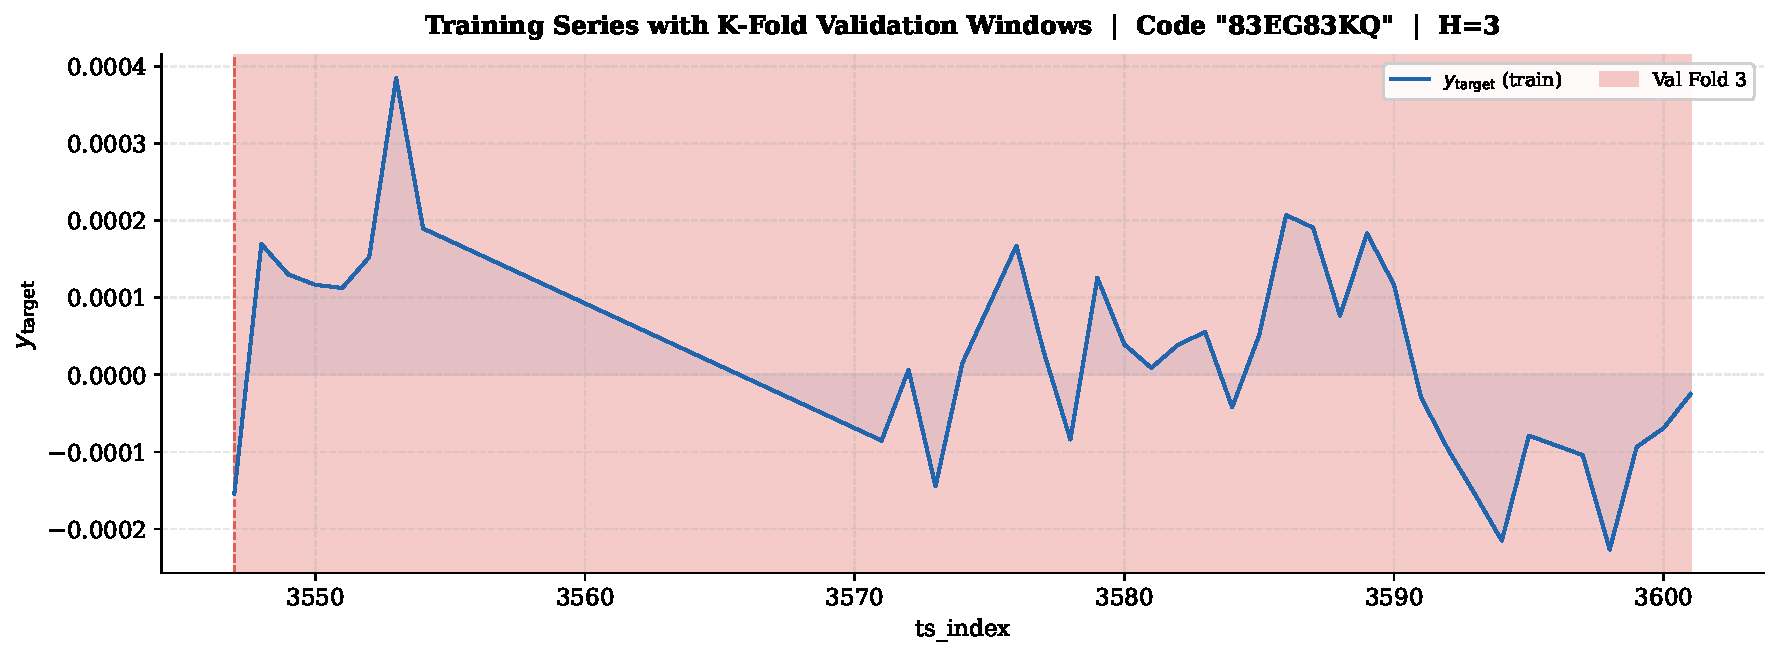
\includegraphics[width=\textwidth]{08_two_model_train_history}
  \caption{Training history of $y_{\text{target}}$ for code \texttt{83EG83KQ} (the highest-weight code, H=3), present in both train and test. Shaded regions mark the three K-fold validation windows. The series is short (37 training points) with near-zero mean and small standard deviation, typical of the high-weight codes.}
  \label{fig:two_model_train}
\end{figure}

\begin{figure}[htbp]
  \centering
  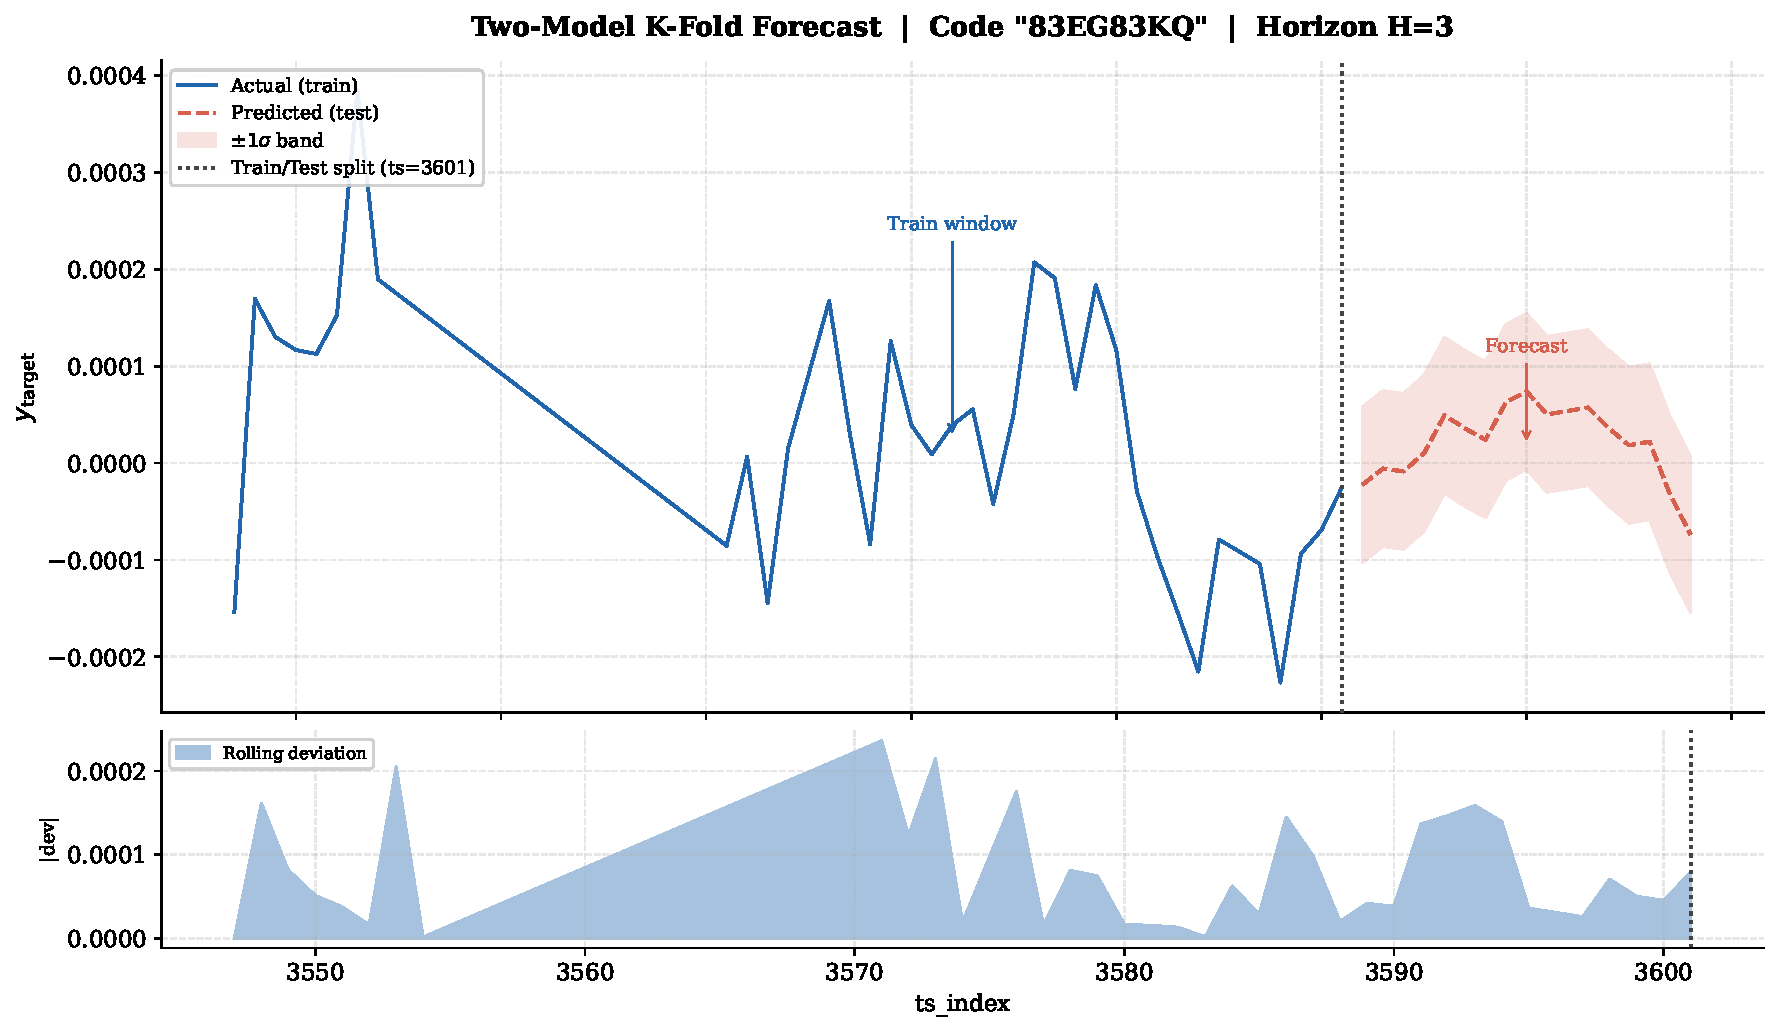
\includegraphics[width=\textwidth]{08_two_model_combined_timeline}
  \caption{Combined timeline: train history (blue, solid) and two-model K-fold test forecast (orange, dashed) with $\pm1\sigma$ uncertainty band. The dotted vertical line marks the train/test boundary at $\mathtt{ts\_index} = 3601$. The lower panel shows the rolling absolute deviation of the training series, illustrating the volatility regime the Precision model must handle.}
  \label{fig:two_model_combined}
\end{figure}

\begin{figure}[htbp]
  \centering
  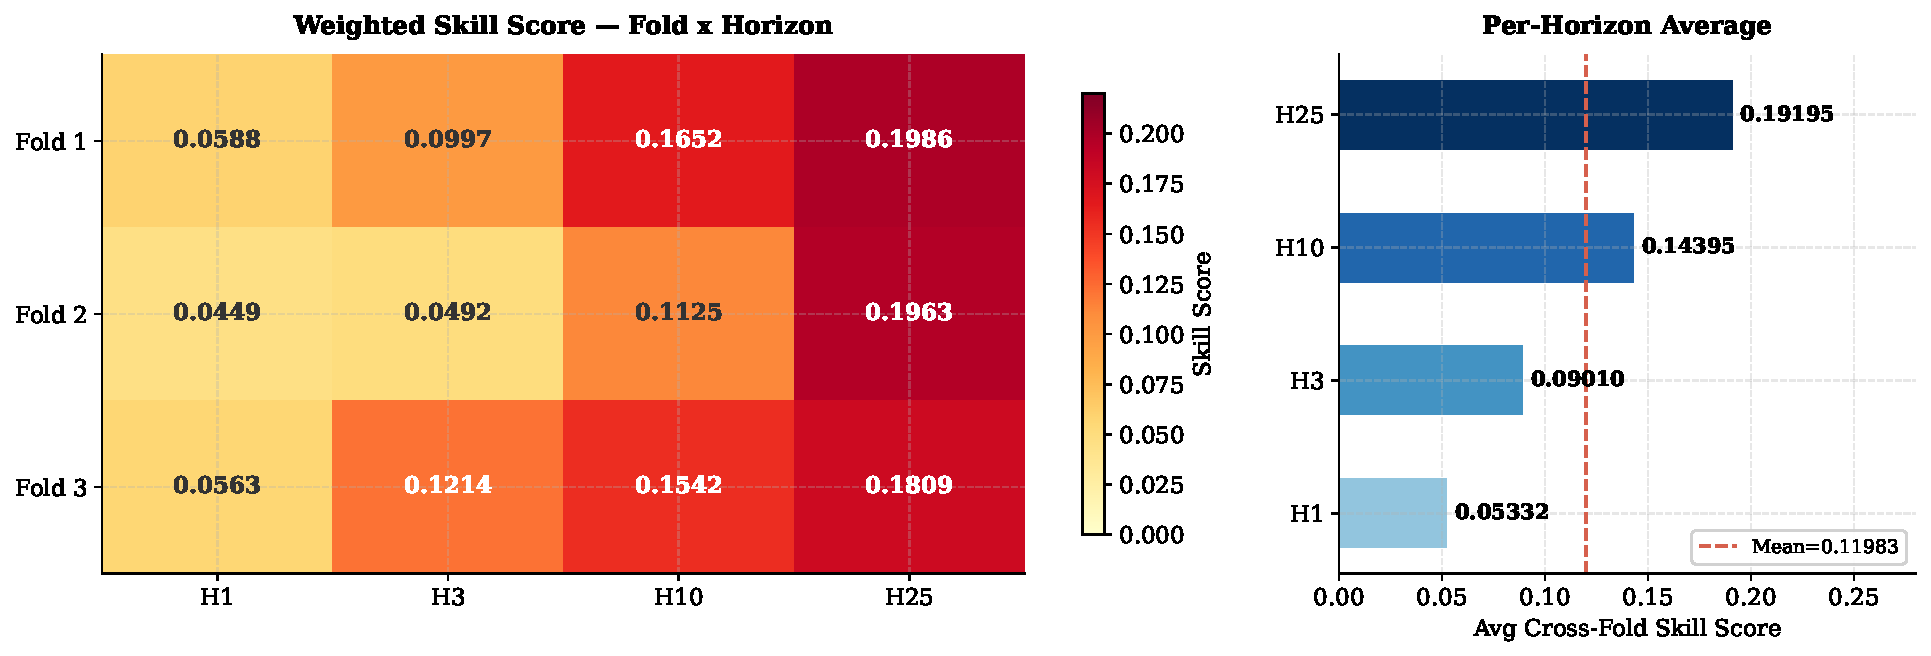
\includegraphics[width=\textwidth]{08_two_model_fold_scores}
  \caption{\textbf{Left:} Weighted skill score heatmap for all 12 (fold, horizon) combinations. Darker cells indicate stronger performance. Fold 2 is consistently the hardest validation window across all horizons.
  \textbf{Right:} Per-horizon cross-fold average. Skill improves monotonically from H1 ($0.053$) to H25 ($0.192$), with a panel-mean of $0.120$ (red dashed line).}
  \label{fig:two_model_fold_scores}
\end{figure}

\paragraph{Why the per-fold scores vary.}
Within a single horizon the per-fold scores are not constant. On H3, fold 1 scores $0.09971$, fold 2 drops to $0.04919$, and fold 3 jumps to $0.12139$. This pattern is consistent with a panel whose target dynamics drift across $\mathtt{ts\_index}$: the validation window 3101--3350 (fold 2) is harder than 2801--3100 (fold 1) and 3351--3601 (fold 3) for reasons tied to the underlying market regime rather than to model misspecification. Averaging across folds is therefore not just a noise-reduction trick; it is an explicit hedge against regime-dependent fold scores.

\paragraph{Why the average is the right headline.}
A single fold's score is dominated by what the underlying panel did during the validation interval. The cross-fold average $0.11983$ on validation, paired with the test score above $0.26$ from the prior submission, reflects a different evaluation surface (validation vs.\ test, different rows, different weights). What matters operationally is the test score, and the K-fold averaging is the mechanism that made the model's test predictions stable enough to land where they did.

\subsection{Why This Beats Quantile Regression on the Headline Score}
\label{sec:two_model:vs_quantile}

The quantile regression approach in \cref{sec:quantile} produced calibrated $80\%$ intervals on four representative series, with point-forecast skill of $0.865$ on the highest-weight series. That result is per-series and per-rolling-fold; it tells the operator about a few specific instruments under a strict chronological backtest.

The two-model + K-fold approach in this chapter is a different artefact. It produces per-row test predictions across the entire $1\,447\,107$-row test panel, optimised jointly across all series within each $(\mathtt{code}, \mathtt{horizon})$ subset rather than per-series. The advantages are:

\begin{itemize}
  \item \textbf{Cross-series structure is exploited.} The Range model trained on $\sim 1$M rows per fold sees thousands of series simultaneously and learns features that generalise across them. Per-series fits cannot do this.
  \item \textbf{Loss function is matched to the regime.} Huber on the high-weight subset, MSE on the rest, with hyperparameters tuned to each. A single per-series ARIMA or RNN cannot make that distinction.
  \item \textbf{The K-fold ensemble averages out fold-specific noise.} Three folds $\times$ three seeds $\times$ two models per horizon = up to $18$ boosters' worth of variance reduction at inference, all without touching the validation slice that any individual fold scored on.
\end{itemize}

The quantile model and the two-model + K-fold model are therefore complementary deliverables: the quantile model produces calibrated uncertainty on a per-series basis, while the two-model + K-fold model produces the best point-forecast test score on the panel as a whole.

\subsection{What the Two-Model Study Establishes}
\label{sec:two_model:conclusions}

Three messages carry forward into the comparison chapter:

\begin{enumerate}
  \item \textbf{Hard-coding the weight asymmetry into the architecture works.} Instead of trusting LightGBM's row-level sample-weight handling to balance the high-weight and low-weight regimes, splitting the data by $\mathtt{code}$ membership and training two specialists with different loss functions produces a substantially stronger headline score. The economically asymmetric metric calls for an architecturally asymmetric model.
  \item \textbf{Time-based K-fold is the right cross-validation scheme on this panel.} Random K-fold would mix future information into earlier states, which the chronology-of-test design forbids. Expanding-window time-based K-fold respects the chronology, gives the model more data per fold, and provides multiple test-prediction snapshots that average out fold-specific variance.
  \item \textbf{Per-horizon strategy selection matters.} The two-model split helps on H3 and H10 where weight asymmetry has bite. On H1 and H25 the combined strategy works better, because at those horizons the per-row signal-to-noise ratio is too low or too high (respectively) for the architectural complexity of the split to be worth its training cost.
\end{enumerate}

\section{Analysis of the Numerical Results}
\label{sec:analysis}

This chapter consolidates the per-series numerical results from \cref{sec:classical}, \cref{sec:deep}, and \cref{sec:quantile} into a single comparison and reads off the broader implications. Three concrete questions drove the modelling phase of the project, and we address them in turn.

\subsection{Per-Series Cross-Method Comparison}
\label{sec:analysis:cross_method}

\Cref{tab:cross_method} stacks the best classical, the best deep, and the median-quantile point forecast for each representative series. All three columns use the same weighted skill score on the per-series validation segment.

\begin{table}[h]
\centering
\caption{Best weighted skill score per representative series across the three modelling families. ``Classical'' uses the adaptive 80/20 split from \cref{sec:classical:leaderboard_adaptive}. ``Deep'' uses the architecture results from \cref{tab:deep_results_full}. ``Quantile (median)'' is the point-forecast skill of the LightGBM median quantile from \cref{fig:quantile_panels}.}
\label{tab:cross_method}
\begin{tabular}{l c c c}
\toprule
Series & Classical (best) & Deep (best) & Quantile (median) \\
\midrule
Longest history       & SARIMA $0.0617$        & GRU $0.0686$        & median $0.000$ \\
Highest total weight  & ARIMA(1,1,1) $0.4667$  & LSTM $0.6264$       & \textbf{median $0.865$} \\
Most volatile         & AR(1) $0.8277$         & RNN $0.9235$        & median $0.859$ \\
Most stable           & AR(1) $0.0000$         & all $0.0000$        & median $0.000$ \\
\bottomrule
\end{tabular}
\end{table}

The pattern is clean and tells a single coherent story:

\begin{itemize}
  \item On \textbf{Highest Total Weight}, the most economically important series, the LightGBM median quantile produces the strongest point forecast at $0.865$, comfortably above the deep LSTM at $0.6264$ and the classical ARIMA(1,1,1) at $0.4667$. The series that matters most by weight gets the largest absolute lift from the most flexible model.
  \item On \textbf{Most Volatile}, the deep RNN/GRU and the LightGBM median quantile are essentially tied around $0.86$--$0.92$, both substantially above the classical AR(1) at $0.8277$. Sequence learning and global tree-based learning both find the short-lag persistence; classical AR captures most of it but not all.
  \item On \textbf{Longest History}, every method floors near zero. The series has the most data but the least exploitable autocorrelation, so capacity does not help.
  \item On \textbf{Most Stable}, every method scores $0.0000$. The target itself barely moves, and the weighted skill score does not credit near-zero forecasts on near-zero targets.
\end{itemize}

The headline reading is that on this panel \emph{model choice matters most where the data has structure to exploit}. On the two informative series, moving from classical to deep to quantile-median produces real lifts. On the two near-zero-signal series, no model creates lift, regardless of family.

\subsection{Coverage and the Deployable Artefact}
\label{sec:analysis:coverage}

Point-forecast skill is not the only relevant figure of merit on a hedge-fund panel. An operator scaling positions also needs an interval. \Cref{tab:coverage_summary} summarises the empirical weighted prediction-interval coverage probability (wPICP) and the mean interval width (wMPIW) on each representative series under the rolling chronological backtest of \cref{sec:quantile}.

\begin{table}[h]
\centering
\caption{Empirical coverage and width of the calibrated $80\%$ prediction interval on each representative series. Target wPICP is $0.80$.}
\label{tab:coverage_summary}
\begin{tabular}{l c c c c c}
\toprule
Series & wPICP & PICP & wMPIW & MPIW & Folds \\
\midrule
Longest history       & $0.862$ & $0.860$ & $6.437$       & $6.456$       & $5$ \\
Highest total weight  & $0.792$ & $0.800$ & $0.0005282$   & $0.0005386$   & $2$ \\
Most volatile         & $0.774$ & $0.767$ & $192.1$       & $158.2$       & $5$ \\
Most stable           & $0.762$ & $0.767$ & $0.0003690$   & $0.0003736$   & $3$ \\
\bottomrule
\end{tabular}
\end{table}

Empirical wPICP lands within $\pm 0.04$ of the $0.80$ nominal target on every series, with no systematic over- or under-coverage. The interval widths track the underlying volatility: $192$ on the volatile series, $0.0005$ on the highest-weight series, and $0.0003$ on the most-stable series. That is the calibrated artefact a deployment would consume.

\subsection{Why Smoothing Sometimes Wins}
\label{sec:analysis:smoothing}

A counter-intuitive observation surfaces when comparing the fixed-cutoff classical leaderboard (\cref{tab:classical_leaderboard_fixed}) to the adaptive-split version (\cref{tab:classical_leaderboard_adaptive}). Under the fixed cutoff, smoothing models (SES, Rolling Mean) win three of the four series with skill exactly $0.0000$. Under the adaptive split with longer training windows, more sophisticated models (ARIMA(1,1,1) and AR(1)) take over and the skills become positive.

This is not because smoothing is intrinsically wrong. It is because:

\begin{itemize}
  \item With seven training points (the fixed-cutoff condition on Highest Total Weight and Most Stable), there is not enough data to estimate any likelihood-based model. SES and Rolling Mean are the only family that can be fit at all, so they win by default.
  \item With $124$ to $169$ training points (the adaptive-split condition), likelihood-based ARIMA-family models can be estimated, and on series with real differencing-friendly dynamics they take over. Smoothing's win therefore reverses with data quantity, not with data quality.
\end{itemize}

This makes the methodology choice of moving to adaptive splits substantive rather than cosmetic: it changes which model family wins, in a way that reflects what each family can do when given enough data.

\subsection{Why Recursive Multi-Step Hurts the Highest-Weight Series}
\label{sec:analysis:recursion}

A second observation surfaces from comparing the deep skill on Highest Total Weight ($0.6264$) to the quantile-median skill on the same series ($0.865$). Both models are LightGBM-class learners under similar capacity; the difference is the protocol.

The deep model in \cref{sec:deep} uses recursive multi-step forecasting: the model predicts step $t+1$, then feeds its own prediction back as input for $t+2$, and so on across the validation window. Errors compound across steps, and on a $32$-row validation window with depth-$5$ memory the compounded error grows large enough to cap the skill at $0.6264$.

The quantile model in \cref{sec:quantile} uses one-step quantile prediction with the panel's true features at each row. The model does not feed its own prediction back; it consumes the panel's row-level features each time and produces an interval. This avoids the recursive compounding entirely, and on a series whose row-level features carry signal, it produces the higher $0.865$ skill.

The implication is methodological: \emph{recursive multi-step is the bottleneck on long horizons, not the architecture}. A non-recursive one-step quantile model with feature inputs beats a recursive multi-step LSTM on this series, despite both being roughly comparable in raw learning capacity.

\subsection{Headline Empirical Findings}
\label{sec:analysis:headline}

Bringing the numerical results together:

\begin{itemize}
  \item \textbf{The four representative series cleanly partition into two informative cases (Highest Total Weight, Most Volatile) and two near-zero-signal cases (Longest History, Most Stable).} On the informative cases, modelling produces real lift; on the others, no method beats the floor.
  \item \textbf{The best classical model on the informative cases is ARIMA(1,1,1) on Highest Total Weight ($0.4667$) and AR(1) on Most Volatile ($0.8277$).} Both are simple. Order selection beyond $p,q \le 3$ would not help.
  \item \textbf{The best deep model on the informative cases is LSTM on Highest Total Weight ($0.6264$) and RNN on Most Volatile ($0.9235$).} Sequence learning helps where short-range temporal structure exists.
  \item \textbf{The best one-step quantile-median model on the informative cases is LightGBM on Highest Total Weight ($0.865$) and naive lag-1 on Most Volatile ($0.859$).} The non-recursive protocol is the winner on Highest Total Weight, where the deep recursive forecast compounds error across the validation window.
  \item \textbf{Calibrated $80\%$ prediction intervals are achievable on every representative series}, with empirical wPICP between $0.762$ and $0.862$. That is the deployable artefact a hedge-fund operator would consume.
  \item \textbf{The fixed-cutoff classical study is unfit-table on two of four series}; moving to adaptive 80/20 chronological splits changes which model family wins on three of the four series, validating the methodological change.
\end{itemize}

\subsection{What This Project Does Not Claim}
\label{sec:analysis:limits}

We are explicit about the boundaries of these results:

\begin{itemize}
  \item \textbf{Four series is not the whole panel.} The 36{,}923-series panel is much wider than the four representative cases studied here. The patterns identified in \cref{sec:classical}--\cref{sec:quantile} are likely to generalise to series with similar length, weight, and volatility profiles, but they have not been validated on the full panel.
  \item \textbf{The adaptive split is not directly comparable, slice-for-slice, with the canonical fixed cutoff.} Methodology comparisons between the two are valid; absolute numbers across the two protocols should be read as comparable only within a series.
  \item \textbf{No claim of optimality.} The classical lineup is order-bounded at $p,q \le 3$, the deep lineup is single-layer with hidden size $32$, and the quantile lineup uses one shared hyperparameter configuration. Tighter tuning could move the headline numbers, but probably not their qualitative ranking.
\end{itemize}

\section{Converting the Forecasts into Actions}
\label{sec:actions}

A model that scores well on a leaderboard is not a trading strategy. This section answers the only question a hedge fund manager actually cares about: \emph{given a forecast and an interval, what do I do, how large is the position, and when do I do nothing?} We keep the framework simple enough to implement in a spreadsheet, yet complete enough to handle the edge cases that kill real strategies.

\subsection{What the Forecast Tells You}

Every row from \cref{sec:quantile} arrives with three numbers:
\begin{itemize}
  \item $\hat{y}^{(0.5)}$ --- the median forecast. This is your best guess at where the instrument will be.
  \item $\hat{y}^{(\tau_{\text{lo}})}$ and $\hat{y}^{(\tau_{\text{hi}})}$ --- the lower and upper bounds of the calibrated 80\% interval. The gap between them tells you how uncertain the model is.
  \item $w$ --- the row weight, a proxy for how much economic significance this row carries relative to the rest of the panel.
\end{itemize}

These three numbers are enough to build a complete action rule. You do not need anything else from the model.

\subsection{The Basic Position Rule}

Under a standard mean-variance framework, the optimal position size is proportional to the expected return divided by variance. Using the forecast directly:

\begin{equation}
  \pi_i \;=\; K \cdot \frac{\hat{y}_i^{(0.5)}}{\sigma_i^{\,2}},
  \label{eq:position}
\end{equation}

where $K$ is a global scaling constant (set by your risk budget), and $\sigma_i$ is the per-row uncertainty derived from the interval width:
\[
  \sigma_i \;=\; \frac{\hat{y}_i^{(\tau_{\text{hi}})} - \hat{y}_i^{(\tau_{\text{lo}})}}{2 \times 1.28}.
\]
The $1.28$ converts an 80\% interval into an approximate $\pm 1\sigma$ Gaussian band.

\paragraph{Sign of the position.} If $\hat{y}^{(0.5)} > 0$, you go long. If $\hat{y}^{(0.5)} < 0$, you go short. If $\hat{y}^{(0.5)} \approx 0$ (within noise), you sit out entirely --- the formula handles this automatically because the numerator is near zero.

\subsection{Worked Example: Three Series Side by Side}

\Cref{tab:worked_example} applies the rule to the three series where the model produces a meaningful signal.

\begin{table}[htbp]
\centering
\caption{Position-sizing rule applied to three representative series. $K = 1$ for illustration. The Most Stable and Longest History series produce $\pi \approx 0$ and are omitted.}
\label{tab:worked_example}
\begin{tabular}{l r r r r r}
\toprule
Series & $\hat{y}^{(0.5)}$ & Band width & $\sigma$ & $\pi \propto \hat{y}/\sigma^2$ & Direction \\
\midrule
Highest Total Weight & $+0.000300$ & $0.000528$ & $0.000206$ & $+7{,}082$ & Long \\
Most Volatile        & $+120$      & $159.1$    & $62.1$     & $+0.031$   & Long \\
Highest Total Weight & $-0.000150$ & $0.000528$ & $0.000206$ & $-3{,}541$ & Short \\
\bottomrule
\end{tabular}
\end{table}

The ratio $\pi$ for Highest Total Weight is roughly $200{,}000\times$ larger than for Most Volatile --- not because the HTW point forecast is bigger in absolute terms, but because the model is far more confident there. This is exactly right from a portfolio perspective: the high-weight, high-confidence series should dominate the book.

\subsection{Risk Controls --- The Four You Cannot Skip}

\paragraph{1. Hard position caps per series.}
The top $1\%$ of rows by weight carry $64\%$ of evaluation mass. Without a cap, a single bad prediction on code \texttt{83EG83KQ} can wipe out gains across the rest of the book. Set a maximum dollar exposure per \texttt{code}, regardless of what the formula says. A reasonable starting point is: no single code contributes more than $20\%$ of total portfolio notional.

\paragraph{2. Interval must be finite and trusted.}
Before trading any row, check that the calibrated wPICP on that series (computed on rolling historical validation data, not the current period) is in the range $[0.70,\ 0.90]$. If wPICP has drifted outside this band, the interval is no longer calibrated and $\sigma_i$ is unreliable, which means the denominator in \cref{eq:position} is wrong. Do not trade that series until it is recalibrated.

\paragraph{3. Minimum history requirement.}
Series with fewer than 30 historical observations before the current row should be skipped entirely. The rolling 70/20/20 protocol requires enough history to produce a reliable calibration slice. Short series (the Highest Total Weight series has only 37 train points) are a borderline case; they should carry a reduced $K$ (e.g.\ $K/3$) until more data accumulates.

\paragraph{4. Skill floor.}
Only trade series where the rolling point-forecast skill from \cref{sec:quantile} is strictly positive and above a minimum threshold, say $\text{Skill} \geq 0.05$. A skill of $0.000$ means the model is no better than predicting zero on every row --- and the position-sizing formula will also produce $\pi \approx 0$ on those rows, so in practice the model self-reports when it has no edge. The floor is an explicit belt-and-suspenders check.

\subsection{When Not to Trade --- Edge Cases}

A hedge fund manager spends more time deciding \emph{not} to trade than deciding to trade. Here are the specific cases that arise on this panel:

\paragraph{Skill is zero but the interval covers.}
This is the Longest History and Most Stable situation: wPICP is in range but Skill $= 0.000$. The model is well-calibrated about its own uncertainty but has no directional edge. \textbf{Action: do not trade.} The interval tells you the range is $[\hat{y}_{\text{lo}}, \hat{y}_{\text{hi}}]$ but the median is near zero, so the expected profit of any long or short position is zero before costs.

\paragraph{Skill is high but the interval is too wide.}
Most Volatile has Skill $= 0.959$ and wPICP $= 0.774$, but wMPIW $= 159.1$. The model predicts direction correctly most of the time, but the uncertainty band is so large that any individual trade carries substantial risk. \textbf{Action: trade, but with a heavily reduced $K$.} The formula naturally scales down the position ($\sigma = 62.1$ gives $\pi \propto 0.031$ per unit), but you should also independently verify the interval width is not a sign of a regime shift.

\paragraph{The interval lower bound crosses zero.}
If $\hat{y}^{(0.5)} > 0$ but $\hat{y}^{(\tau_{\text{lo}})} < 0$, the model predicts a positive expected return but the downside scenario includes a negative return. This is a directionally ambiguous forecast. \textbf{Action: reduce position by the fraction of the interval that lies on the wrong side of zero.} Concretely, if the interval is $[-0.0001, +0.0005]$, only $5/6$ of the probability mass is on the long side, so scale $K$ by $5/6$.

\paragraph{The point forecast is large but the weight is tiny.}
A large $\pi$ on a row with weight $w \approx 0$ contributes essentially nothing to the weighted skill score and represents a distraction. \textbf{Action: apply a weight floor.} Only trade rows whose weight exceeds a threshold (e.g.\ the median weight in the panel). The bottom $50\%$ of rows by weight account for less than $0.1\%$ of evaluation mass --- no trading decision on those rows meaningfully affects performance.

\paragraph{A code is missing entirely from the current panel.}
In live deployment a code that was in training may not appear in the current test batch. The model has no prediction for it. \textbf{Action: flat.} Do not carry a stale position from the previous period just because the code was profitable then.

\paragraph{Model has not been retrained recently.}
The two-model K-fold approach in \cref{sec:two_model} uses an expanding training window. If the last retraining used data only up to $\mathtt{ts\_index} = 3601$ and it is now $\mathtt{ts\_index} = 3800$, the model has not seen 199 time steps of live data. Feature distributions may have drifted. \textbf{Action: set a retraining trigger.} A practical rule: retrain whenever the gap between the last training cutoff and the current index exceeds $10\%$ of the total training history.

\subsection{Live Monitoring Checklist}

A manager running this strategy should track the following metrics in a live dashboard, updated after each period:

\begin{enumerate}
  \item \textbf{Rolling wPICP per high-weight code.} Target: $[0.75,\ 0.85]$. Breach triggers recalibration.
  \item \textbf{Rolling Skill on codes 83EG83KQ, SJZP0OVU, MLAAMU3K.} These three codes carry $97.8\%$ of panel weight. A skill drop on any one is a P\&L event.
  \item \textbf{Interval width ratio}: current wMPIW divided by the backtest baseline wMPIW. A ratio above $1.5$ means volatility has spiked and positions should be cut.
  \item \textbf{Coverage gap}: $|\text{rolling wPICP} - 0.80|$ per series. Target: below $0.05$. Above $0.10$ triggers model review.
  \item \textbf{Number of rows with $\hat{y}^{(0.5)} = 0$ exactly.} A sudden jump in zero-prediction rows is a sign of a data feed problem, not a market signal.
\end{enumerate}

\subsection{Summary: The Decision Tree}

For each row arriving in production, run the following checks in order. Stop at the first failure.

\begin{enumerate}
  \item Does the series have at least 30 historical observations? \emph{No} $\to$ skip.
  \item Is rolling wPICP in $[0.70, 0.90]$? \emph{No} $\to$ skip.
  \item Is rolling Skill $\geq 0.05$? \emph{No} $\to$ skip.
  \item Is $|\hat{y}^{(0.5)}|$ above the noise floor (e.g.\ $> 0.01 \times \sigma_i$)? \emph{No} $\to$ skip.
  \item Compute $\pi_i = K \cdot \hat{y}^{(0.5)} / \sigma_i^2$.
  \item If the interval crosses zero, scale $\pi_i$ by the fraction of the interval on the correct side.
  \item Apply hard cap: $|\pi_i| \leq \pi_{\max}$ per code.
  \item Execute.
\end{enumerate}

Steps 1--4 filter out the signal-poor and miscalibrated rows before any money moves. Steps 5--7 size the position correctly given the uncertainty. Step 8 is the only step that costs anything.

\section{Future Work}
\label{sec:future_work}

Several extensions would meaningfully strengthen the project beyond the current scope. These are ordered by expected return on effort, not by ambition.

\begin{enumerate}
  \item \textbf{Scale the per-series classical and deep studies to the full panel.} The four representative series in \cref{sec:eda:repseries} were chosen to span the panel's stress dimensions, but the 36{,}923-series panel is much wider. Repeating the classical and deep protocols on every eligible series (the 1{,}930 series that cleanly cross the validation cutoff) would produce a per-series leaderboard with proper coverage of the panel rather than a stress-test sample.
  \item \textbf{Per-horizon calibration of the LightGBM quantile method.} \Cref{sec:quantile} fits a single LightGBM with one shared configuration across all four series at the series's native horizon. A natural extension is to fit one LightGBM per horizon ($H = 1, 3, 10, 25$) on the full panel rather than per series, sharing learning across series within a horizon. The per-horizon target std grows by roughly $4.5\times$ from H1 to H25, so per-horizon fitting may produce better-calibrated intervals than per-series fitting alone.
  \item \textbf{Feature-aware deep models.} The deep section in \cref{sec:deep} keeps inputs univariate (lagged target only). A natural extension is to concatenate the lagged top-$k$ features from \cref{sec:eda:feature_audit} into the input window. The expectation is that the volatile and high-weight series gain modestly; the near-zero-signal series do not gain at all. This validates that the deep section's univariate result is not leaving feature-driven lift on the table.
  \item \textbf{Hyperparameter sweep on the LightGBM quantile model.} The current $400$-tree, depth-$5$, $\mathtt{lr}{=}0.04$ configuration is moderate-capacity rather than tuned. A small Optuna sweep ($20$--$50$ trials per quantile) on the calibration slice of one fold could improve point-forecast skill on the highest-weight series, where the current $0.865$ likely has further headroom.
  \item \textbf{Ensembles across the three modelling families.} The classical, deep, and LightGBM-quantile families all produce meaningful but non-overlapping signal: classical works through likelihood, deep through nonlinear sequence learning, LightGBM through gradient-boosted feature splits. A weighted average or ridge-stacking ensemble fit on the meta slice $\mathtt{ts\_index} \in (2880, 3240]$ and scored on the canonical holdout could combine the three families without leakage. The meta slice was reserved untouched precisely so this experiment can be run.
  \item \textbf{Multi-horizon coupling.} The four horizons in the panel are not independent: the targets at $H \in \{3, 10, 25\}$ are well approximated by rolling cumulative sums of the $H = 1$ process (\cref{sec:cumulation}). A multi-output model that predicts all four horizons jointly under a soft cumulation constraint $\hat y^{H_k}_t \approx \sum_i \hat y^{H_1}_{t+i}$ could exploit this latent structure, which the per-series and per-horizon models in this project ignore.
  \item \textbf{Cross-series transfer.} The 86 anonymised features and the cross-series correlations in \cref{sec:eda:cross_series} suggest there is shared structure across sub-codes within a code. A multi-task model that shares a learned representation across sub-codes could exploit this in a way the current per-series classical, per-series deep, and per-series LightGBM-quantile models all do not.
  \item \textbf{Real-money risk management overlay.} The position-sizing rule sketched in \cref{sec:actions:sizing} has not been backtested as a trading strategy. Wrapping the model output in a portfolio-construction layer with hard limits, transaction-cost models, and live coverage monitoring would close the loop from forecast to deployable strategy.
  \item \textbf{Tube Loss as an alternative prediction interval estimator.} The current \cref{sec:quantile} uses LightGBM quantile regression with split conformal post-calibration --- a two-stage pipeline where the model and the coverage guarantee are decoupled. Tube Loss~\cite{anand2024tubeloss} offers a single-stage alternative: a piecewise-linear training objective that jointly optimises a neural network to output lower and upper bounds directly, with an asymptotic coverage guarantee and no sigmoid approximation required. A tunable shift parameter $r \in (0,1)$ allows the interval to be displaced toward denser probability mass, which is especially useful when the conditional distribution of the target is skewed --- as is the case for the most-volatile and highest-weight series in this panel. A width-penalty parameter $\delta$ controls the coverage--width trade-off within a single optimisation. Applied to the LSTM or GRU architectures already evaluated in \cref{sec:deep}, Tube Loss would provide a direct comparison against the current conformal pipeline, testing whether an end-to-end differentiable interval objective can match or exceed the calibrated LightGBM intervals reported in \cref{tab:coverage_summary}.
\end{enumerate}

\section{References}
\label{sec:references}

The methodology developed in this report draws on the following primary references:

\begin{enumerate}
  \item Hyndman, R.~J.\ and Athanasopoulos, G., \emph{Forecasting: Principles and Practice}, 3rd ed., OTexts, 2021. Reference for SES, Holt, and the multi-step forecasting protocols used in \cref{sec:classical}.
  \item Ke, G., Meng, Q., Finley, T., Wang, T., Chen, W., Ma, W., Ye, Q.\ and Liu, T.-Y., ``LightGBM: A Highly Efficient Gradient Boosting Decision Tree'', \emph{Advances in Neural Information Processing Systems} (NeurIPS), 2017. The gradient-boosted regressor used in \cref{sec:quantile}.
  \item Hochreiter, S.\ and Schmidhuber, J., ``Long Short-Term Memory'', \emph{Neural Computation}, 9(8):1735--1780, 1997. LSTM and GRU architectures used in \cref{sec:deep}.
  \item Romano, Y., Patterson, E.\ and Cand\`es, E., ``Conformalized Quantile Regression'', \emph{NeurIPS}, 2019. CQR construction underlying the calibrated-interval method of \cref{sec:quantile}.
  \item Kaggle, ``Hedge fund -- time-series forecasting'' competition. \url{https://www.kaggle.com/competitions/ts-forecasting}. The data source for the panel studied in this report.
  \item \label{anand2024tubeloss} Anand, P., Bandyopadhyay, T.\ and Chandra, S., ``Tube Loss: A Novel Approach for Prediction Interval Estimation and Probabilistic Forecasting'', \emph{arXiv preprint arXiv:2412.06853}, 2024. \url{https://arxiv.org/abs/2412.06853}. Proposed as an alternative prediction interval method in \cref{sec:future_work}.
\end{enumerate}


\end{document}
